\documentclass[12pt]{article}
\usepackage{natbib}
\usepackage[english, french]{babel}
\usepackage[utf8]{inputenc}
\usepackage[T1]{fontenc}
\usepackage{tikz}
\usepackage{amsmath}
\usepackage{textcomp}
\usepackage{graphics}
\usepackage{graphicx}
\usepackage{multirow}
\usepackage{url}
\usepackage{psfrag}
\usepackage{fancyhdr}
\usepackage{vmargin}
%\usepackage[backend=biber]{biblatex}
\usepackage{csquotes}
\usepackage[hidelinks]{hyperref}
\usepackage{enumitem}
\usepackage[justification=centering]{caption}
\usepackage{array,multirow,graphicx}
\usepackage{float}
\usepackage{mathtools}
\usepackage{graphicx}
\usepackage{caption}
\usepackage{ifthen}
\usepackage{color}
\usepackage{xcolor}
\usepackage{listings}
%\usepackage[nottoc, notlof, notlot]{tocbibind}

\def\rot#1{\rotatebox{90}{#1}}

\DeclarePairedDelimiter\ceil{\lceil}{\rceil}
\DeclarePairedDelimiter\floor{\lfloor}{\rfloor}

%\titleformat{\chapter}[display]{\normalfont\bfseries}{}{0pt}{\Huge}\titlespacing*{\chapter}{0pt}{-50pt}{17pt}

%%%%%%%%%%%%%%%%%%%%%%%%%%%%%%%%%%%%%%%%%%%%%%%%%%%%%%%%%%%%%%%%%
\definecolor{codegreen}{rgb}{0,0.6,0}
\definecolor{codegray}{rgb}{0.5,0.5,0.5}
\definecolor{codemauve}{rgb}{0.58,0,0.82}
\definecolor{backcolour}{rgb}{0.99,0.99,0.99}

\lstdefinestyle{codestyle}{
	backgroundcolor=\color{backcolour},   
	commentstyle=\color{codegreen},
	keywordstyle=\color{blue},
	numberstyle=\tiny\color{codegray},
	stringstyle=\color{codemauve},
	basicstyle=\ttfamily\footnotesize,
	breakatwhitespace=false,         
	breaklines=true,                 
	captionpos=b,                    
	keepspaces=true,                 
	numbers=left,                    
	numbersep=5pt,                  
	showspaces=false,                
	showstringspaces=false,
	showtabs=false,                  
	tabsize=2
}
\lstset{style=codestyle}
%%%%%%%%%%%%%%%%%%%%%%%%%%%%%%%%%%%%%%%%%%%%%%%%%%%%%%%%%%%%%%%%%

\setmarginsrb{1.5 cm}{1 cm}{1.5 cm}{1 cm}{0.51 cm}{1 cm}{0.5 cm}{1 cm}
\setlength{\parindent}{1cm}

\title{Algorithmes pour l'analyse du SARS-CoV2}
\author{Omar, Céline, Chaima et Mathis}
\date{November 2020}

\makeatletter
\let\thetitle\@title
  \let\theauthor\@author
\let\thedate\@date
\makeatother

\pagestyle{fancy}
\fancyhf{}
\rhead{\theauthor}
\lhead{\thetitle}
\cfoot{\thepage}


\begin{document}

\begin{titlepage}
    \centering
    
 	
\includegraphics[scale=0.36]{logo_TN_horizontal}\\[1.0 cm]
 	
	\textsc{\LARGE Télécom Nancy}\\[1.5 cm]
	\textsc{\Large Rapport de Projet TAPS}\\[0.5 cm]
	%\textsc{\large code de l'UE}\\[0.5 cm]
	{\large \thedate}\\[0.5 cm]
	\rule{\linewidth}{0.2 mm} \\[0.5 cm]
	{ \huge \bfseries \thetitle}\\[0.2 cm]
	\rule{\linewidth}{0.2 mm} \\[1.5 cm]
	\textsc{\large Groupe 13}\\[1.0 cm]
	
	\begin{minipage}{0.4\textwidth}
		\begin{flushleft} \large
		\emph{Étudiants:}\\
			Mohamed Omar CHIDA \\
			Mathis DUMAS \\
			Chaima TOUNSI OMEZZINE \\
			Céline ZHANG
		\end{flushleft}
	\end{minipage}~
	\begin{minipage}{0.4\textwidth}
		\begin{flushright} \large
		\emph{Numéro Étudiant:}\\
			31730598 \\
			32012997 \\
			32025001 \\
			32024925
		\end{flushright}
	\end{minipage}\\[1.4 cm]
	
	\large
	\emph{Encadrants du projet :}\\
	   Olivier FESTOR\\
	   Sébastien DA SILVA\\
	   Gérald OSTER\\
	   Titouan CARETTE\\[1.5 cm]

	
\includegraphics[scale=0.15]{logo_UL_horizontal}\\[1.5 cm]

	\vfill
\end{titlepage}

\section*{Remerciements}
Nous tenons à remercier chaque membre de l'équipe pour leurs contributions à la réalisation de ce projet. Nous tenons à remercier également Madame Sophie Mézières pour son aide concernant l'implémentation de la fonction calculant les quartiles. Nous aimerions remercier, de plus, Markus Piotrowski, un contributeur de la bibliothèque \texttt{BioPython} qui nous a aidé pour l'utilisation du module \texttt{pairwise2} et du module \texttt{PairwiseAligner}. Nous aimerions remercier les encadrants du projet pour nous avoir guidé durant ce projet, et notamment pour leurs réponses aux e-mails.\\[2.5 cm]

%\newpage

\begin{abstract}
    Dans le cadre de l'étude des algorithmes et de leur application, nous avons été chargés de faire des travaux de recherches sur la génomique, en particulier concernant le virus SARS-CoV-2, et de mettre en œuvre différentes méthodes (implémentations d'algorithmes, de fonctions) pour l'analyse du génome du SARS-CoV2. Ce virus est à l'origine de la pandémie mondiale 2020. Une analyse statistique des nucléotides et des acides aminés des séquences d'ARNm du génome a d'abord été réalisée. Ensuite, des algorithmes nécessaires à l'étude ont été mis en œuvre, tels que la distance de Levenshtein pour mesurer la distance minimale d'édition et l'algorithme de Needleman-Wunsch pour calculer un alignement optimal des séquences. Une poignée d'autres diverses outils ont également été mis en œuvre pour faciliter les tests et les analyses comparatives.
\end{abstract}

\renewcommand{\abstractname}{Abstract}

\begin{abstract}
In the context of the study of algorithms and their application, we have been assigned to search and implement different methods and algorithms that will allow the analysis of the genome of SARS-CoV-2 the virus that spread widely at the beginning of 2020 starting a global pandemic. A statistical analysis of the genome nucleotides and it's amino acids was first conducted. Followed by the implementation of the tools and algorithms necessary such as the Levenshtein algorithm for measuring the minimal edit distance and Needleman-Wunsch for optimal sequence alignment. Handful of other utilities and miscellaneous tools has also been implemented to facilitate testing and benchmarking. 
\end{abstract}

\newpage

\tableofcontents

\newpage



\section*{Introduction} 
    \addcontentsline{toc}{section}{Introduction}

%https://fr.wikipedia.org/wiki/Acide_ribonucl%C3%A9ique_messager#Synth%C3%A8se_et_maturation
%https://fr.wikipedia.org/wiki/Pand%C3%A9mie_de_Covid-19
%https://media.kartable.fr/uploads/finalImages/final_58a5c51e11c6a1.12021277.png
%https://www.annabac.com/sites/annabac.com/files/depot/images/PB_Bac_SVT_1re_2019_9782401052222/05222_C02_F07_01.png
%http://phage-t4-tpe.e-monsite.com/pages/i-les-virus/la-replication-des-virus.html

Dans le cadre de notre module de TAPS, il nous est proposé un projet nous permettant d'acquérir et de mettre en oeuvre des compétences en gestion de projet et en programmation dynamique au travers d'un cahier des charges ayant pour finalité le développement et l'application d'algorithmes pour l'analyse de séquences génomiques du virus du SARS-CoV2 à l'origine de la pandémie de COVID-19.\\

L'objectif de ce projet est de réaliser des outils informatiques permettant l'étude des caractéristiques des séquences du génome SARS-CoV2, de les appliquer à des échantillons de séquences, d'étudier leur complexité théorique, de les tester sur toutes sortes de situation, et d'effectuer des tests de performances pour les comparer à la complexité théorique. Tout d'abord, nous devons faire un ensemble de fonctions qui permettra une analyse de statistique descriptive des séquences de nucléotides du génome. Ensuite, en réalisant une fonction codons, qui transformera les séquences de nucléotides en séquences d'acides aminés, nous allons faire une même analyse sur les séquences d'acides aminés. Puis, dans le but d'étudier les différences entre les séquences d'acides aminés, nous allons implémenter une fonction calculant la distance de Levenshtein, cela nous donnera la distance entre deux séquences. Enfin, pour afficher les similitudes entre deux séquences, nous réaliserons une fonction utilisant l'algorithme de Needleman-Wunsch, cette fonction permet d'afficher les alignements des séquences du génome. Pour ce faire, nous devons coder en \textsf{python}, nous avons à disposition pour les tests, les bibliothèques \texttt{pytest}, \texttt{timeit}, \texttt{biopython}, ce dernier est un outil particulier dans le domaine de la bio-informatique.\\

Les résultats du projet sont présentés dans ce rapport, il y a une partie consacrée à l'état de l'art, c'est-à-dire la présentation des notions en biologie, et l'explication théorique des procédés utilisés, une partie consacrée à l'implémentation et l'application de l'algorithme, elle explique le raisonnement entre les lignes de codes, et présente les résultats lors de l'exécution des codes. Dans ce rapport se trouve également une partie pour les tests et les performances des fonctions réalisées, ainsi que les comparaisons à la complexité théorique calculée dans la partie implémentation; une partie présentant la gestion de projet de l'équipe, les moyens utilisés. À la fin de ce rapport, se trouve une partie pour les annexes, dans laquelle se trouve les déclarations de non-plagiat, les tableaux d'organisation du travail, les comptes rendus de réunions, et d'autres divers documents.

\newpage 

\subsection*{Cahier des charges}
    \addcontentsline{toc}{subsection}{Cachier de charges}
    \begin{table}[!h]
        \centering
        \begin{tabular}{|l|}
            \hline
            Travaux demandés \\
            \hline
            Fonctions d'analyses statistiques \\
            Application des fonctions d'analyses sur les séquences de nucléotides \\
            Fonction \texttt{codons} \\
            Application des fonctions d'analyses sur les séquences de codons \\
            Fonction distance de Levenshtein \\
            Application de la fonction distance de Levenshtein sur les séquences de codons \\
            Fonctions algorithme Needleman-Wunsch (un seul alignement, tous les alignements) \\
            Afficher les opérations de l'algorithme Needleman-Wunsch \\
            Calcul de complexité \\
            Tests des fonctions réalisées \\
            Mesures de performances des fonctions \\
            \hline
        \end{tabular}
        \caption{Le cahier des charges}
        \label{tab:cdc}
    \end{table}

\subsection*{Mentions légales}
    \addcontentsline{toc}{subsection}{Mentions légales}
Ce projet n’est pas destiné à un usage commercial, ainsi, les images présentés, notamment les images de tests, d'applications ou de gestion de projet, ne sont pas destinées à la publication. \\
Cependant, le caractère strictement scolaire de ce projet nous autorise à les inclure en accord avec :
\begin{itemize}
\item Code civil : articles 7 à 15, article 9 : respect de la vie privée
\item Code pénal : articles 226-1 à 226-7 : atteinte à la vie privée
\item Code de procédure civil : articles 484 à 492-1 : procédure de référé
\item Loi n78-17 du 6 janvier 1978 : Informatique et libertés, Article 38
\end{itemize}
Les déclarations sur l’honneur de non-plagiat des membres de l’équipe du projet sont présentés dans les quatres premières pages de l'annexe.

Cette version\footnote{version 1} du rapport a été finalisée le 5 Janvier 2021.

\newpage


\section{État de l'art}
L'épidémie de COVID-19~\cite{pandemie}~a débutée à Wuhan en Chine le 17 Novembre 2019. Aujourd'hui, cette pandémie à contaminée plus de 80 millions d'individus et à fait 1,75 millions de victimes. Des laboratoires du monde entier étudient de près le coronavirus SARS-CoV-2, virus vecteur de cette pandémie, dans le but de mettre au point un vaccin. Pour ce faire, les chercheurs se basent sur l'analyse du génome du virus.\\

Chaque être vivant possède un génome : il s'agit de l'ensemble du matériel génétique codé dans son ADN~\cite{adn} ou dans son ARN~\cite{arn} dans le cas de certains virus, comme pour le SARS-CoV-2 en l'occurence. Le génome comprend notamment les gènes codant des protéines dont les organismes ont besoin pour assurer le bon fonctionnement de leur cellules. L'ADN (Acide DésoxyriboNucléique) est une macromolécule composée d'une chaîne de molécules appelés nucléotides. Les nucléotides composant l'ADN sont l'adénine (A), la guanine (G), la thymine (T) et la cytosine (C). C'est donc cette succession de nucléotides qui compose le génome et donc les gènes~\cite{rnaw}.\\
Pour synthétiser une protéine, la cellule transcrit d'abord le gène codant la protéine cherchée (une séquence d'ADN donc), en ARN pré-messager (ARNpm), c'est la transcription~\cite{rnatrc}. L'ARN (Acide RiboNucléique) est donc aussi une macromolécule composée d'une succession de nucléotides, à l'exception de la thymine (T) qui est remplacée par l'Uracile (U). La transcription se fait par complémentarité des nucléotides : A est associé à U, T est associé à A, G est associé à C et C est associé à G. La transcription de la séquence d'ADN "GTAC" serait donc la séquence d'ARN "CAUG" (CF fig.\ref{fig:schema_transcription}).\\

\begin{figure}[!h]
    \centering
    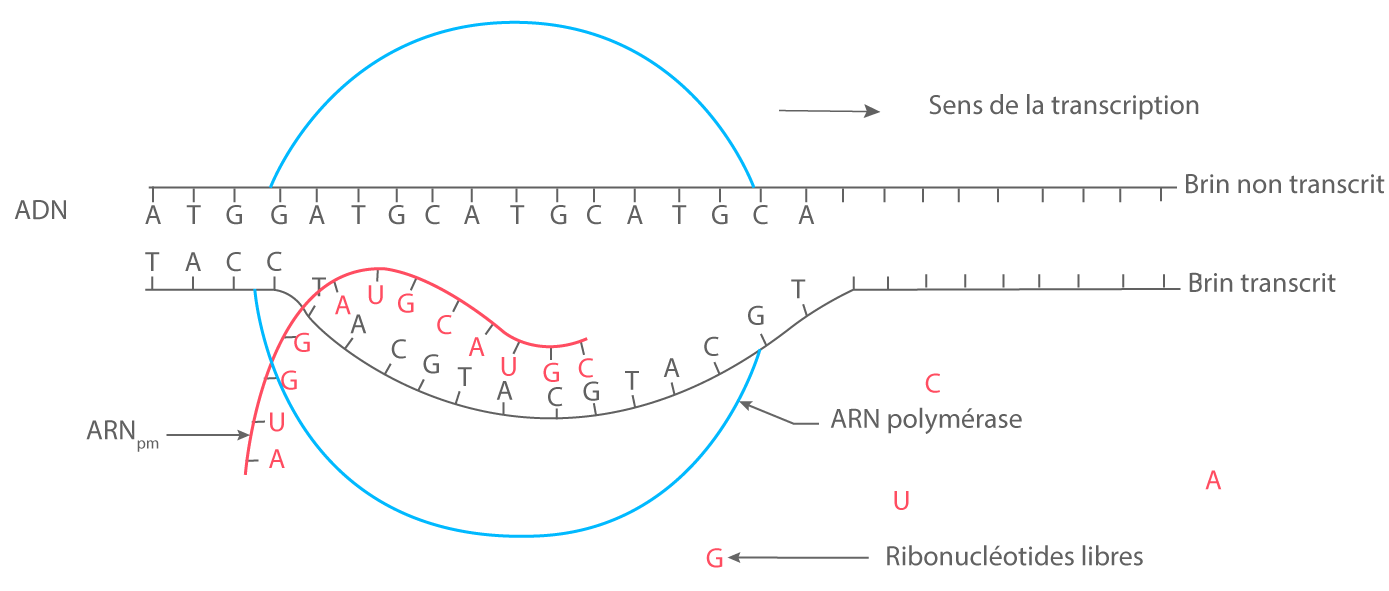
\includegraphics[scale = 0.37]{Images/Intro/transc.png}
    \caption{Schéma du processus de transcription}
    \label{fig:schema_transcription}
\end{figure}


Le brin d'ARN ainsi obtenu est appellé ARN pré-messager (ARNpm). Le gène transcrit comporte des régions codantes (exons) et des régions non-codantes (introns) pour la fabrication de la protéine. Ainsi, il est nécessaire d'enlever du brin d'ARNpm les introns pour obtenir un brin d'ARNm~\cite{arnm} : c'est la phase d'épissage~\nocite{epissage} (CF fig.\ref{epissage}).\\

\begin{figure}[!h]
    \centering
    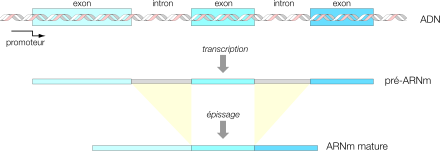
\includegraphics[scale = 1.1]{Images/Intro/epissage.png}
    \caption{Schéma du processus d'épissage}
    \label{epissage}
\end{figure}

\newpage

L'ARNm obtenu est ensuite traduit~\cite{rnat} en protéine par le ribosome. Une protéine est une macromolécule formée d'une succession de molécules appellées acides aminés. Le ribosome parcourt le brin d'ARNm et lit les nucléotides trois par trois. Chaque triplet de nucléotides est apellé codon. Le ribosome commence la traduction au premier codon START qu'il lit, et associe ensuite à chaque codon l'acide aminé correspondant pour former ainsi la chaine d'acides aminés. Une fois arrivée sur un codon STOP, le ribosome se décroche et la chaine d'acide aminés obtenue se plie sur elle même pour former la protéine voulue~(CF fig.\ref{traduction})\nocite{traduction}.\\

\begin{figure}[h!]
    \centering
    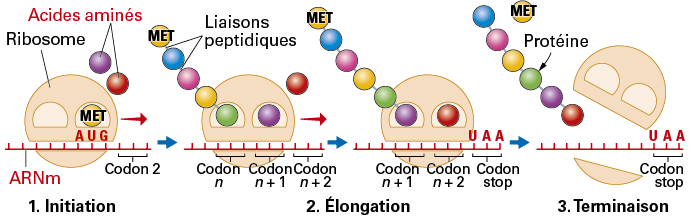
\includegraphics[scale = 1.4]{Images/Intro/Trad.png}
    \caption{Schéma du processus de traduction}
    \label{traduction}
\end{figure}



Les virus sont des agents infectueux qui utilisent une cellule hôte pour se multiplier selon le processus de réplication~\cite{replication}. Ils prennent généralement la forme de capsules contenant du matériel génétique, de l'ARN dans le cas du coronavirus SARS-CoV-2. Lors de la réplication, le virus se colle à la paroi d'une cellule hôte et fusionne avec elle, libérant ainsi son ARN dans la cellule infectée. Naturellement, les ribosomes vont traduire l'ARN présent dans la cellule, et ainsi former de nouvelles particules virales, qui seront ensuite encapsulées et libérées de la cellule infectée pour aller en infecter de nouvelles~\nocite{dnatr}(CF fig.\ref{replication}).\\

\begin{figure}[h!]
    \centering
    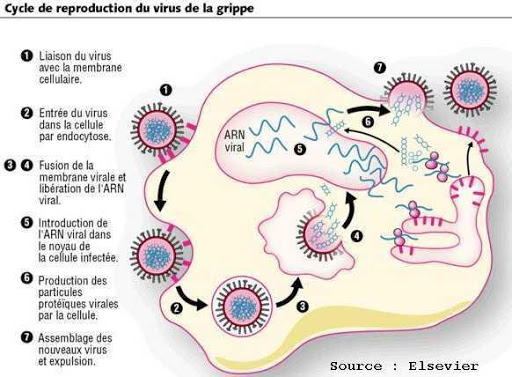
\includegraphics[scale = 0.8]{Images/Intro/replication.jpg}
    \caption{Schéma du processus de réplication}
    \label{replication}
\end{figure}

\newpage

En génomique, plusieurs algorithmes ont été mis au point pour analyser, caractériser, sélectionner et comparer des séquences d'ADN. C'est ainsi que l'on peut retrouver des liens de parentés entre les différentes espèces d'animaux ou bien, dans le cadre de ce projet, ceci nous permet d'identifier les caractéristiques du génome SARS-CoV2, de comparer les différentes séquences du génome entre elles et éventuellement d'observer les différentes mutations subies par le virus SARS-CoV2.


\subsection{Analyse descriptive d'une séquence génomique} 
Les analyses permettant de décrire les séquences du génome sont les fonctions de stastistiques descriptives, la moyenne, la médiane, les quartiles, la variance, l'écart-type, l'intervalle interquartile et éventuellement la notion de proportion. Le but est d'appliquer ces fonctions à un échantillon (groupe de séquences d'ARNm) ceci va nous donner des valeurs qui estiment le profil général des ARNm du SARS-CoV2.

On suppose un échantillon de taille $N$ donné, on peut appliquer l'analyse statistique sur des variables quantitatives, par exemple la taille des séquences et le nombre de chaque nucléotide des séquences de l'échantillon, ou bien sur des variables qualitatives, par exemple le nombre de nucléotides (A, U, G, C) d'une séquence (en proportion).
\paragraph{La moyenne} (dite moyenne arithmétique) notée $\bar{X}$ d'une variable discrète associé à un caractère sur une population (ou un échantillon) de taille (effectif) N est le rapport de la somme des valeurs $X_i$ prises par cette variable pour chaque élément de la population (ou de l'échantillon) sur l'effectif total de celle-ci~\cite{stats}. 
    \begin{equation}
        \bar{X} = \frac{X_1 + X_2 + ... + X_N}{N}
        \label{moy}
    \end{equation}
Par exemple, la moyenne $\bar{X_c}$ de la liste de pointures de chaussures (35, 36, 38, 39, 39, 40, 40, 42, 43) est~:
    \[\bar{X_c} = \frac{35 + 36 + 38 + 39 + 39 + 40 + 42 + 43}{8} = 39\]
Dans l'analyse du génome, nous appliquons cela sur la taille des séquences du génome et le nombre des nucléotides, donc la moyenne est la somme de la taille des séquences (resp. le nombre d'un nucléotide) de l'échantillon, noté $X_i$, sur le nombre de séquence de l'échantillon noté $N$.

\paragraph{La proportion} notée $P_i$ d'une caractéristique spéficique à l'étude d'un caractère est le rapport du nombre d'apparition de cette caractéristique sur l'effectif total~\cite{stats}. Par exemple, la proportion d'un nucléotide dans une séquence est le nombre de nucléotide $i$ sur la taille de la séquence noté $n$. En effet, la somme des proportions de tous les nucléotides vaut 1.
    \begin{equation}
        P_i = \frac{\textbf{nombre~de~nucléotides}~i}{n}
        \label{prop}
    \end{equation}
Par exemple, dans une soirée, on note le nombre de personne en couple $N_{CP}$ et célibataire $N_S$ dans cette liste ($N_{CP}$: 8 , $N_S$: 12), les proportions des personnes en couple $P_{CP}$ et des personnes célibataire $P_{S}$ sont la suivante~:
    \[P_{CP} = \frac{8}{20} = 0,4\] et \[P_{S} = \frac{12}{20} = 0,6\] de plus \[P_{CP} + P_{S} = 0,4 + 0,6 = 1\]
        

\paragraph{La médiane} d'une variable décrivant un caractère au sein d'une population (resp. d'un échantillon) est la valeur dont 50\% des éléments sur le caractère étudié lui sont inférieurs et 50\% lui sont supérieurs~\cite{stats}. Si plusieurs valeurs peuvent être candidates, on prend la moyenne entre la plus petite valeur et la plus grande.\\
En particulier, lorsque nous avons une variable quantitative discrète, nous étudions, par exemple, dans un ensemble de 5 individus, la taille en mètre des individus est donnée par la liste suivante (1,70 ; 1,58 ; 1,65 ; 1,70 ; 1,81).\\
Nous trions la liste, ce qui donne (1,58 ; 1,65 ; 1,70 ; 1,70 ; 1,81) et la valeur du milieu de la liste correspond à notre médiane, dans notre cas 1,70 est la médiane.\\
Cependant, si nous avons une liste de longueur paire, par exemple (1,58 ; 1,65 ; 1,70 ; 1,81), les valeurs 1,65 et 1,70 peuvent être candidates, ainsi nous prenons la moyenne entre le plus petit candidat et le plus grand comme médiane, dans notre cas c'est la moyenne de 1,65 et 1,70 donc 1,675 est notre médiane.

\paragraph{Les quartiles} d'une variable discrète décrivant un caractère dans une population (resp. un échantillon sont, en général, au nombre de trois~\cite{quart}~: $Q_1$, $Q_2$, $Q_3$. $Q_2$ n'est autre que la médiane. $Q_1$ est la valeur dont 25\% des valeurs prises par la variable lui sont inférieures et 75\% lui sont supérieures. $Q_3$ est la valeur dont 75\% des valeurs prises par la variable lui sont inférieures et 25\% lui sont supérieures. Losrqu'il y a plusieurs candidats possible, nous choisissons le plus petit pour le premier quartile $Q_1$ (l'interpolation par la plus petite valeur) et le plus grand pour le troisième quartile pour $Q_3$ (l'interpolation par la plus grande valeur).\\
En particulier, si nous regardons par exemple le nombre de chocolats reçus à Noël parmi un groupe d'amis, on donne la liste triée (30, 90, 95, 100).\\
30 et 90 sont des candidats pour le premier quartile $Q_1$, mais nous choisissons l'interpolation par la plus petite valeur, donc $Q_1 = 30$.\\
95 et 100 sont des candidats pour le troisième quartile $Q_3$, mais nous choisissons l'interpolation par la plus grande valeur, donc $Q_3 = 100$.\\

\paragraph{L'écart interquartile} noté $\Delta Q$ est la différence entre le troisième et le premier quartile~\cite{EI}.
    \begin{equation}
        \Delta Q = Q_3 - Q_1
        \label{intquart}
    \end{equation}
Il nous permet de calculer la dispersion des valeurs d'un caractère étudié dans population (ou de l'échantillon). Comme le choix de l'interpolation pour $Q_1$ et $Q_3$ est la plus extrême, la valeur de la dispersion (l'intervalle interquartile) est la plus large.\\
Dans l'exemple précédent des chocolats, l'écart interquartile $\Delta Q_c$ est~:
\[\Delta Q_c = 100 - 30 = 70\]

\paragraph{La variance et l'écart-type} sont aussi des indicateurs de dispersion~\cite{dispersion}. La variance notée $Var(X)$ d'une variable discrète $X$ associée à un caractère d'une population (resp. un échantillon) de taille $N$ est définie comme suit, où les $X_i$ sont les valeurs que prend $X$ et $\bar{X}$ est sa valeur moyenne~:
    \begin{equation}
        Var(X) = \frac{1}{N} \sum_{i=1}^{N} (X_i-\bar{X})^2
        \label{var}
    \end{equation}
L'écart-type noté $\sigma$ de la variable $X$ est la racine carré de la variance de la variable $X$.
    \begin{equation}
        \sigma = \sqrt{Var(X)}
        \label{ecartt}
    \end{equation}
Toujours dans l'exemple des chocolats (30, 90, 95, 100), calculons la variance et l'écart-type de cette liste. On note $\bar{X_c}$ la moyenne du nombre de chocolat, $V_c$ la variance du nombre de chocolats dans cette liste, et $\sigma_c$ son écart-type.
    \[\bar{X_c} = \frac{30 + 90 + 95 + 100}{4} = 78,75\]
    \[V_c = \frac{1}{4}[(30 - 78,75)^2 + (90 - 78,75)^2 + (95 - 78,75)^2 + (100 - 78,75)^2] \approx 804,69\]
    \[\sigma_c \approx 28,37\]

\subsection{Les codons} 
 
Afin de décrire plus spécifiquement le génome, on va passer de l'analyse descriptive des échantillons d'ARNm à l'analyse descriptive des échantillons de séquences d'acides aminés. Le but est alors de générer ces séquences. \\
En effet, les acides aminés sont des molécules qui, combinées entre-elles, forment les protéines. Ces protéines sont produites dans la cellules par lecture du code génétique contenu dans l'ADN (les bases A, T, C, G). \\
D'abord, on procède à la transcription de la séquence d'ADN pour obtenir une séquence d'ARNm (les bases A, U, C, G). Ensuite, le ribosome, qui est l'usine à protéine de la cellule, se charge  d'établir des liens entre la séquence d'ARNm et la séquence d'acides aminés à produire en mettant en place un système de lecture. Et enfin, on procède à la traduction en suivant les étapes~\cite{synthpep}~suivantes~: \\


\begin{itemize}
\item  Le ribosome lit un codon~\cite{codon} (3 nucléotides successifs dans une séquence d'acide ribonucléique messager ARNm),
\item  On capte l'acide aminé correspondant à ce codon dans le milieu environnant, en suivant la table~\ref{fig:table des codons ARN}, par l'intermédiaire de l'ARN de transfert. Celui-ci est un ARN comptant une centaine de nucléotides et portant un acide aminé,\\

        \begin{table}[!h]
             \centering
             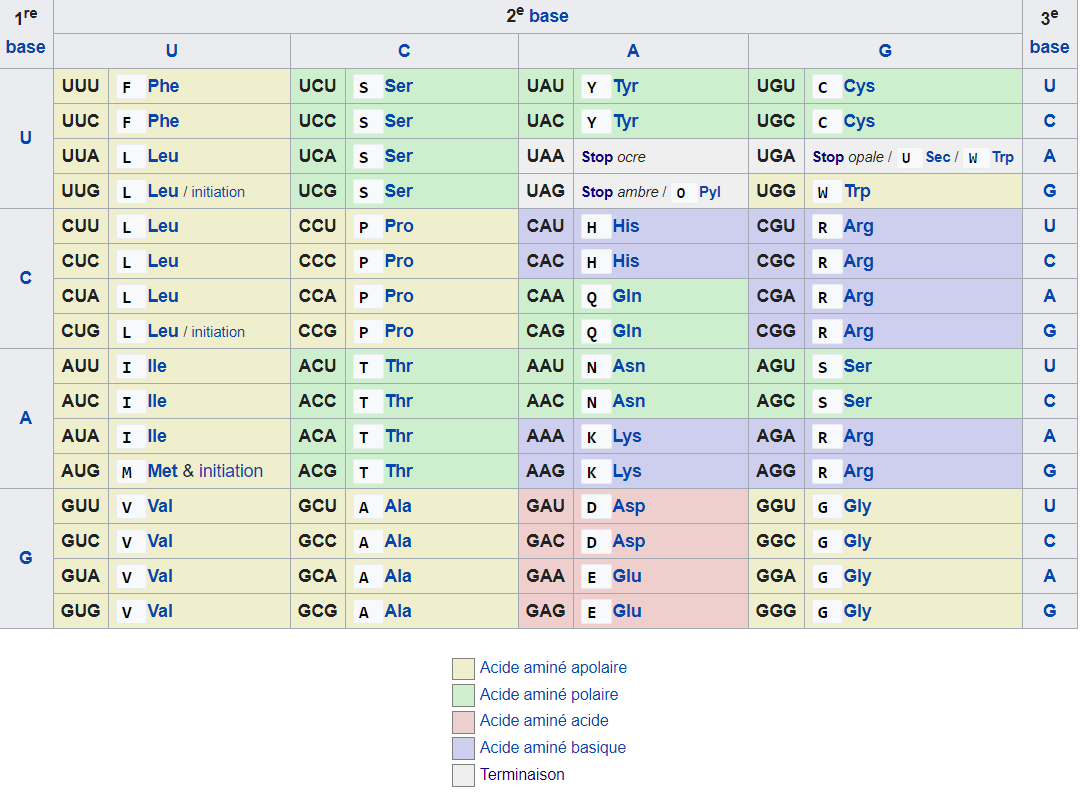
\includegraphics[scale = 0.8]{Images/Codons/tableau des codons ARN.png}
             \caption{Table des codons ARN}
             \label{fig:table des codons ARN}
        \end{table}

\item on ajoute l'acide aminé à la chaine d'acides aminés par la formation des liaisons péptidiques,
\item le ribosome lit ensuite le codon suivant et le cycle se reproduit.
\end{itemize}

Mais, il faut bien noter que le ribosome reconnait~\cite{synth} des codons START (AUG) et des codons STOP (UAA, UAG et UGA) entre lesquels ce processus est effectués (figure \ref{fig:Le processus de traduction}). C'est ainsi qu'on obtient les séquences de protéine qui sont plus descriptives du génome.\\

\newpage

        \begin{figure}[!h]
             \centering
             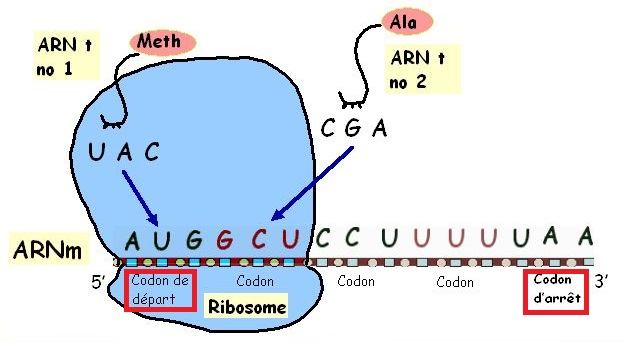
\includegraphics[scale = 0.7]{Images/Codons/traduction.jpg}
             \caption{Le processus de la traduction}
             \label{fig:Le processus de traduction}
        \end{figure}
        

De plus, pour les nucléotides, il existe plus de quatre codes IUPAC~\cite{nucl}  de base (A, G, C , T ou U) comme indiqué sur la table \ref{fig:table des codes IUPAC} ce qui rend le processus plus compliqué.\\

        \begin{table} [!h]
             \centering
             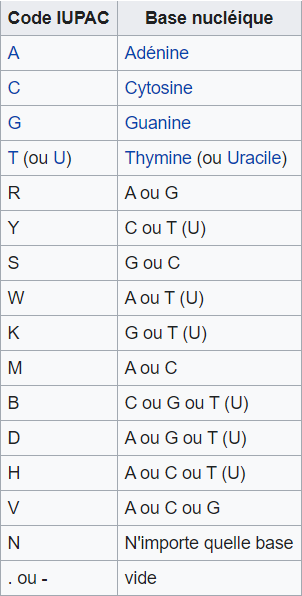
\includegraphics[scale = 1]{Images/Codons/nucleotides.png}
             \caption{Table des  codes IUPAC}
             \label{fig:table des codes IUPAC}
        \end{table}
        
\newpage

\subsection{Distance de Levenshtein} 

%https://fr.wikipedia.org/wiki/Distance_de_Levenshtein


La distance de Levenshtein est une mesure mathématique de la distance entre deux mots, phrases ou ici séquences d'ARN. Concrètement, cette distance correspond au nombre minimal de lettres à ajouter, supprimer ou remplacer pour obtenir une égalité entre les deux chaînes de caractères.\\
Ce sont Wagner et Fischer qui, en 1974, mettent au point l'algorithme calculant cette distance de Levenstein entre deux chaînes de caractères. Cet algorithme est un exemple de programmation dynamique.
En génomique, la distance de Levenstein peut être utilisée pour calculer un "score" de similarité entre deux séquences de nucléotides ou d'acides aminés, et ainsi identifier différents degrés de parenté entre différents génomes. D'autres applications sont envisageables, notamment en reconnaissance vocale.\\

L'algorithme prend en entrée deux chaînes de caractères $seq1$ et $seq2$ (ici "maison" et "long"), de longueur $m$ et $n$ (ici 6 et 4) respectivement. La phase d'initialisation consiste à créer une matrice (ici nommée "dp" pour dynamic programming) vide de dimension $(m+1)\times (n+1)$ et d'attribuer à chaque case de la première ligne le numero de la colonne correspondante et à chaque case de la première colonne le numéro de la ligne correspondante.

\begin{figure}[!h]
    \centering
    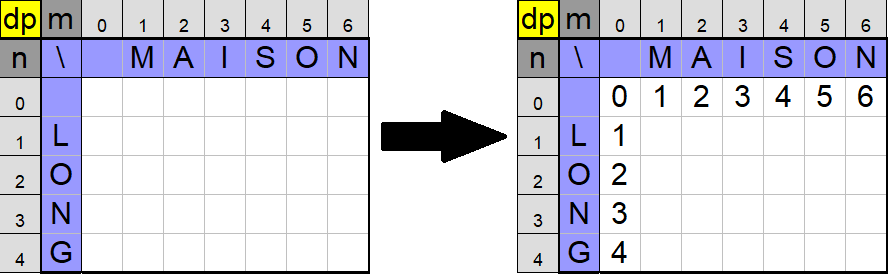
\includegraphics[scale = 0.7]{Images/Levenstein/pre init levenstein.png}
    \caption{Phase d'initialisation de l'algorithme de Wagner et Fischer}
    \label{fig:Phase d'initialisation de l'algorithme de Wagner et Fischer}
\end{figure}

Ensuite, on remplit chaque case, ligne par ligne ou colonne par colonne, en respectant la formule suivante :\\

$dp(i,j)_{(1,1)\leq (i,j)\leq (n,m)} = min\left\{
\begin{array}{ll}
dp(i-1,j)+1\\
dp(i,j-1)+1\\
dp(i-1,j-1) +1 & \mbox{si } seq1(m)\neq seq2(n) \\
dp(i-1,j-1) & \mbox{si } seq1(m) = seq2(n) \\
\end{array}
\right.$\\\\

En reprenant l'exemple, le calcul de $dp(1,1)$ se fait ainsi : on constate d'abord que $seq1(1)\neq seq2(1)$ car "L" n'est pas "M". Ainsi, dp(1,1) prend la valeur minimum entre $dp(0,1)+1=1+1=2$, $dp(1,0)+1=1+1=2$ et $dp(0,0)+1=0+1=1$. Donc $dp(1,1)$ prend la valeur $1$.\\

\begin{figure}[!h]
    \centering
    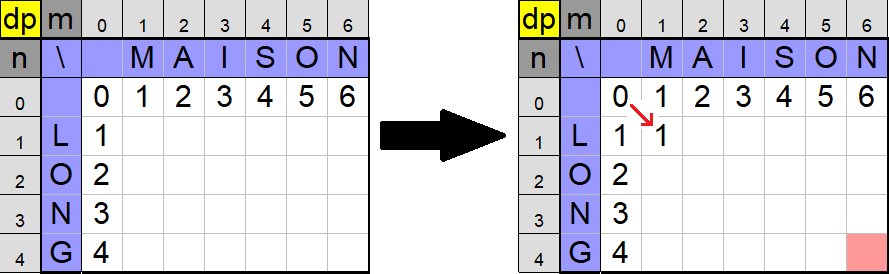
\includegraphics[scale = 0.69]{Images/Levenstein/remplissage levenstein.png}
    \caption{Remplissage de la matrice "dp"}
    \label{fig:Remplissage de la matrice "dp"}
\end{figure}

Concrètement, prendre la valeur du dessus correspond à effacer une lettre, prendre la valeur de gauche correspond à insérer une lettre et prendre la diagonale correspond soit à une substitution (si elles ne sont pas identiques), soit à la conservation des lettres.\\

\newpage

Voici donc la matrice complétée de l'exemple précédent :

\begin{figure}[!h]
    \centering
    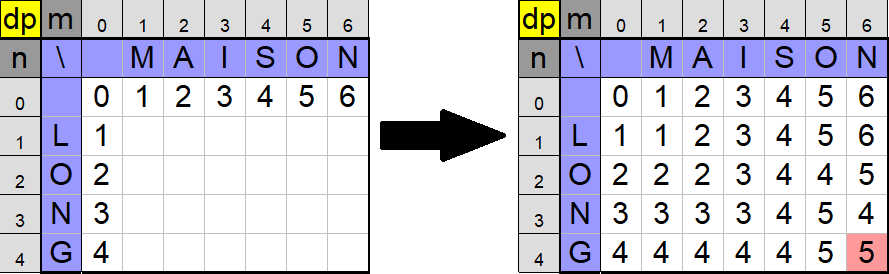
\includegraphics[scale = 0.69]{Images/Levenstein/levenstein rempli.png}
    \caption{Matrice "dp" complète}
    \label{fig:Matrice "dp" complète}
\end{figure}

Finalement, on retrouve notre distance de Levenstein dans la case $(n,m)$ de la matrice ainsi obtenue. Dans l'exemple précédent, la distance de Levenstein entre "maison" et "long" est donc 5.\\

Il est éventuellement possible d'ajouter une table des coûts en paramètre, pour modifier les coûts de suppression, d'addition ou de substitution des lettres : on peut considérer par exemple qu'une substitution coûte 2 dans le sens où elle s'apparente à une suppression puis une addition. Evidemment, les résultats obtenus ne seront pas tout à fait les mêmes, ce qui permet de personnaliser l'algortihme selon les préférences de l'utilisateur.\\
Par exemple, mettre un fort coût de suppression et d'addition avec un faible coût de substitution donnera une distance plus courte entre deux mots de même taille, même si leurs lettres sont différentes etc...



\subsection{Algorithme de Needleman-Wunsch}
\label{subsec:algo_nw} 
%https://fr.wikipedia.org/wiki/Algorithme_de_Needleman-Wunsch


L'algorithme de Needleman-Wunsch est un algorithme permettant de réaliser un alignement de chaînes de caractères avec un recouvrement maximal de ces dernières~\cite{nwcours}. \\
Cet algorithme est un exemple de programmation dynamique pour la résolution de problème d'optimisation, tout comme l'algorithme de Wagner et Fischer, auquel il est apparenté.\\
Son utilisation en génomique est évidente puisqu'il permet d'effectuer des alignements de séquences d'ADN ou d'ARN, qui nous perttent d'identifier les régions semblables entre deux génomes, ainsi que les lieux où ces séquences ont subies des mutations, notamment pour le génome du virus SARS-CoV2 dans le cadre de ce projet~\cite{alignement}.

L'algorithme prend en entrée deux chaînes de caractères $seq1$ de longueur $n$ et $seq2$ de longueur $m$, ainsi qu'un tableau de score contenant les scores à attribuer dans le cas d'un match (les deux caractères correspondent), mismatch (les deux caractères ne correspondent pas) et gap (un caractère est mis en face d'un espace). Voici ci-dessous un exemple d'alignement pour les mots "maison" et "long", ainsi que le calcul du score associé~:\\

\begin{figure}[!h]
    \centering
    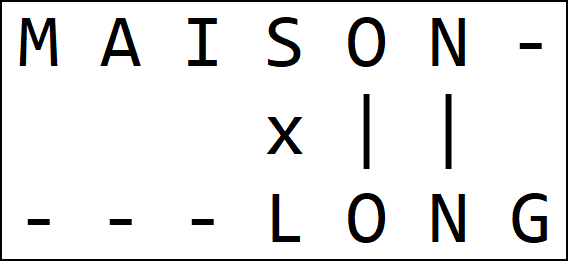
\includegraphics[scale = 0.55]{Images/Needleman/exemple alignement.png}
    \caption{Exemple d'un alignement entre les mots "maison" et "long", les barres représentent un match, la croix un mismatch et les tirets un gap.}
    \label{fig:Exemple d'un alignement entre les mots "maison" et "long", les barres représentent un match, la croix un mismatch et les tirets un gap.}
\end{figure}

En prenant un tableau de score attribuant $1$ point par match, $-1$ par gap et $-5$ par mismatch et en l'appliquant sur l'alignement ci-dessus, on obtient un score de -7.\\

L'algorithme de Needleman-Wunsch se déroule en trois temps. D'abord, une phase d'initialisation, qui ressemble d'assez près à celle de l'algorithme de Wagner et Fischer~: on crée une matrice de dimension $(n+1)\times (m+1)$ et on attribue à chaque case de la première ligne le numéro de la colonne correspondante multiplié par le coût d'un gap et inversement pour la première colonne. \\

\begin{figure}[!h]
    \centering
    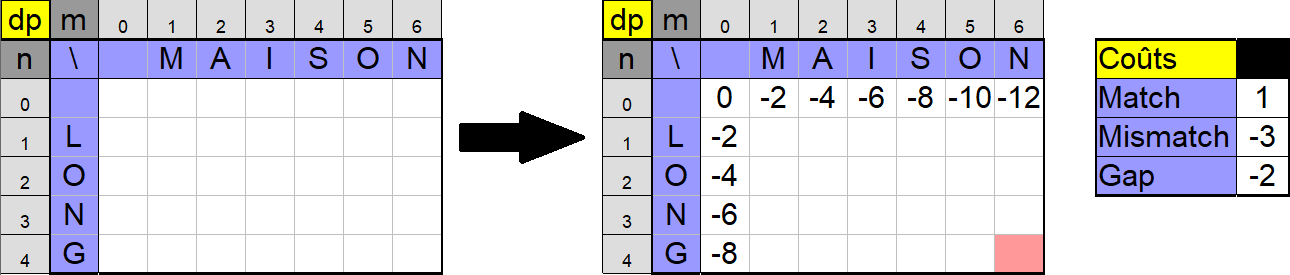
\includegraphics[scale = 0.55]{Images/Needleman/init needleman.png}
    \caption{Initialisation de l'algorithme de Needleman-Wunsch pour les mots "maison" et "long", en utilisant la table de coûts adjacente.}
    \label{fig:Matrice "dp" complète}
\end{figure}

Ensuite, on passe à la phase de remplissage de la matrice de la même manière que pour l'algorithme de Wagner et Fischer, mais en suivant plutôt cette formule ci: \\\\

$dp(i,j)_{(1,1)\leq (i,j)\leq (n,m)} = max\left\{
\begin{array}{ll}
dp(i-1,j)+cout\: Gap\\
dp(i,j-1)+cout\: Gap\\
dp(i-1,j-1) + cout\: Mismatch & \mbox{si } seq1(m)\neq seq2(n) \\
dp(i-1,j-1) + cout\: Match & \mbox{si } seq1(m) = seq2(n) \\
\end{array}
\right.$\\\\

\newpage

En reprenant l'exemple, le calcul de $dp(1,1)$ se fait ainsi : on constate d'abord que $seq1(1)\neq seq2(1)$ car "L" n'est pas "M". Ainsi, dp(1,1) prend la valeur maximum entre $dp(0,1)-2=-2-2=-4$, $dp(1,0)-2=-2-2=-4$ et $dp(0,0)-3=0-3=-3$.\\
Donc $dp(1,1)$ prend la valeur $-3$.\\

On obtient finalement la matrice "dp" remplie suivante :

\begin{figure}[!h]
    \centering
    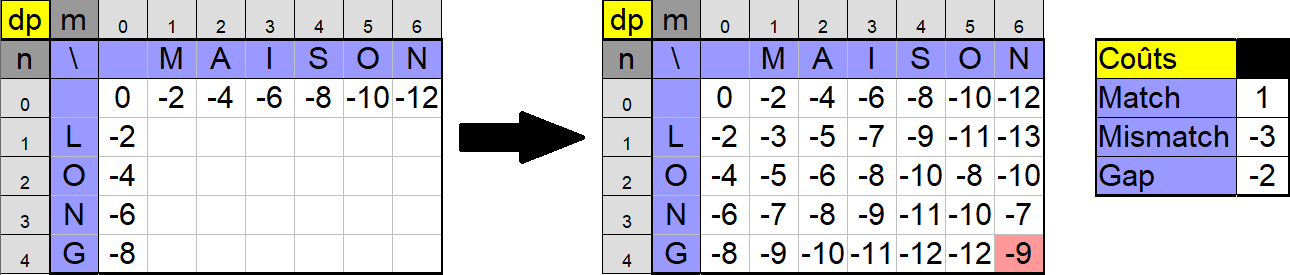
\includegraphics[scale = 0.55]{Images/Needleman/needleman rempli.png}
    \caption{Matrice "dp" remplie pour les mots "maison" et "long" en utilisant la table de coûts illustrée.}
    \label{fig:Matrice "dp" remplis pour les mots "maison" et "long" en utilisant la table de coûts illustrée.}
\end{figure}

Tout comme pour l'algorithme de Wagner et Fischer, on retrouve dans la case en bas à gauche le score maximal pour l'alignement des deux séquences $seq1$ et $seq2$, qui est ici $-9$.\\

Finalement, on passe à la troisième et dernière phase de l'algorithme qui est le "traceback". Maintenant que nous avons rempli la matrice et déterminé le meilleur score possible pour l'alignement des deux séquences, il faut retrouver le chemin qui a permis d'arriver à ce score. Il s'agit concrètement de se positionner sur la case en bas à droite (de coordonnée $(n,m)$), et de remonter la matrice jusqu'à la case en haut à gauche (de coordonnée $(0,0)$), en passant par la ou les cases utilisées pour calculer la valeur de la case dans laquelle on se trouve.\\

Voici, représenté par des traits rouges, l'ensemble des chemins possibles pour le traceback de la matrice "dp" :\\

\begin{figure}[!h]
    \centering
    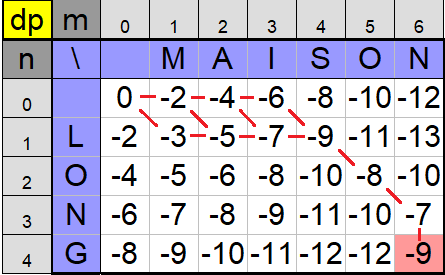
\includegraphics[scale = 0.85]{Images/Needleman/chemins needleman.png}
    \caption{Illustration des chemins possibles à emprunter pour le traceback de la matrice "dp" pendant l'alignement des mots "maison" et "long".}
    \label{fig:Matrice "dp" remplis pour les mots "maison" et "long" en utilisant la table de coûts illustrée.}
\end{figure}

\newpage

Voici comment il faut "lire" le traceback de la matrice "dp" présentée ci-dessus:\\
La case en bas à gauche, $dp(4,6)$, tient sa valeur de $dp(3,6)$. On effectue un déplacement vertical vers le haut, ce qui correspond à placer un gap en face du "G" de "long".\\
La case $dp(3,6)$ tient sa valeur de $dp(2,5)$. On effectue ici un déplacement diagonal, ce qui correspond à placer le "N" de "long" en face du "N" de "maison", c'est un match. Idem pour "O", ce qui nous mène en $dp(1,4)$.\\

On constate ensuite que $dp(1,4)$ peut posséder deux origines : soit elle prend sa valeur de $dp(0,3)$, ce qui correspond à mettre le "L" de "long" en face du "S" de "maison" (mismatch); soit elle prend sa valeur de $dp(1,3)$, ce qui correspond à mettre un gap en face du "S" de "maison".\\

Ainsi, une fois arrivé jusqu'à $dp(0,0)$ l'algorithme est terminé et il renvoie deux chaînes de caractères de même longueur, composées de successions de lettres et de gaps, qui correspondent donc au meilleur (ou un des meilleurs alignements si plusieurs existent) alignement possible pour $seq1$ et $seq2$, étant donné la table de score entrée en paramètre.\\

En reprenant l'exemple, il y a donc quatre alignements optimaux pour les mots "maison" et "long", avec un score de match de +1, un score de mismatch de -3 et un score de gap de -2 :

\begin{figure}[!h]
    \centering
    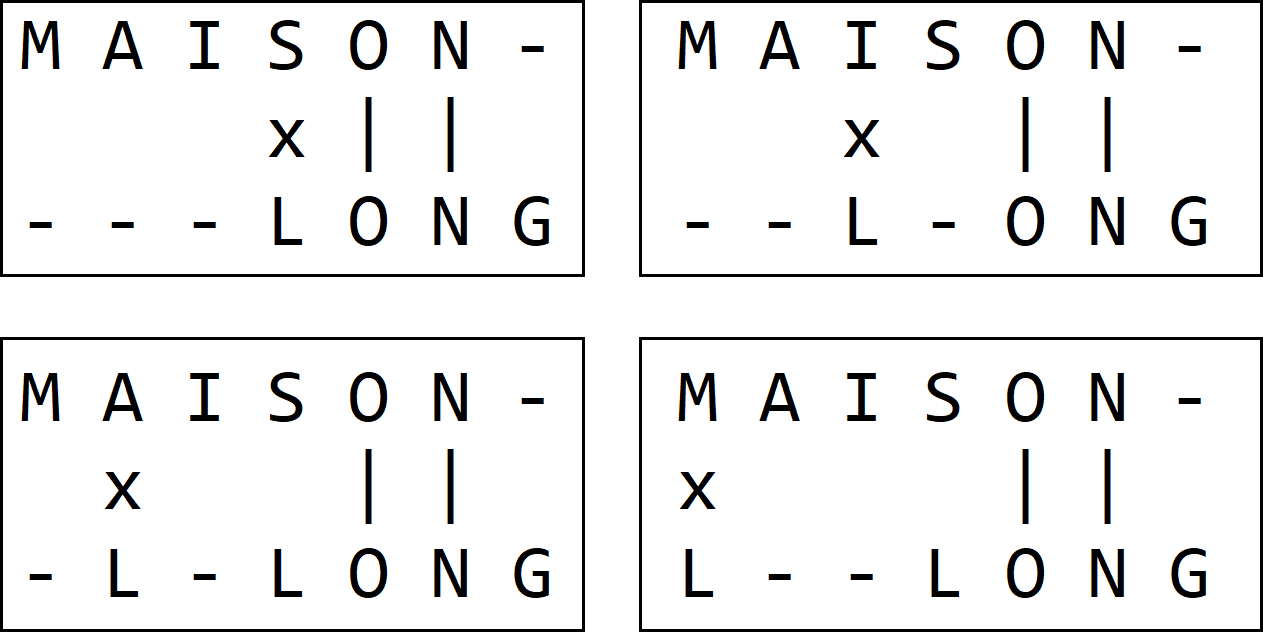
\includegraphics[scale = 0.5]{Images/Needleman/alignements needleman.png}
    \caption{Les quatres meilleurs alignements pour les mots "maison" et "long" avec comme coûts \texttt{match=1}, \texttt{mismatch=-3} et \texttt{gap=-2}.}
    \label{fig:Matrice "dp" remplis pour les mots "maison" et "long" en utilisant la table de coûts illustrée.}
\end{figure}

Dans la pratique, on ajoute souvent un coût d'extension de gap, pour faire en sorte que chaque gap consécutif coûte moins cher que le premier gap de la série (-5 pour le premier gap et -1 pour tout gap consécutif suivant par exemple). Cet ajout favorise donc les grandes séquences de gap plutôt que de nombreuses petites. Ceci est essentiel pour pouvoir aligner un génome avec un gène : on aura une série de gaps au début, jusqu'à ce que la séquence du gène corresponde avec celle du génome, puis à nouveau une série de gaps jusqu'à la fin de la séquence du génome~\cite{alignmit}.\\

\newpage

\section{Implémentation et application des algorithmes} 
Dans cette partie, nous implémentons les fonctions et les algorithmes présentés dans l'état de l'art. L'objectif est d'expliquer la structure du code, les choix des données, des variables, des paramètres, de présenter les applications réalisées pour chaque partie du projet, et de donner la complexité théorique de ces codes.



\subsection{Les fonctions de description statistique}
La plupart des fonctions d'analyse statistique sont simples à implémenter, les plus grandes difficultés sont le choix des types d'interpolation pour les fonctions calculant les quartiles, le choix de la structure des fonctions qui répondent aux demandes du sujet ainsi que l'application sur des échantillons.




\subsubsection{Élaboration des fonctions statistiques}
L'écriture des fonctions calculant les quartiles, ne peuvent pas être faites n'importe comment. Il faut choisir une interpolation\footnote{donne une unique solution} à nos fonctions puis rédiger les tests en conséquence. De ce fait, après renseignement, nous avons choisi (comme décrit dans l'état de l'art) la plus petite valeur pour le premier quartile $Q_1$ et la plus grande pour le troisième quartile $Q_3$. Ceci donnera donc le plus large écart interquartile $\Delta Q$. Ainsi, pour les tests, on peut utiliser dans la bibliothèque \texttt{numpy}, la fonction \texttt{quantile} qui prend en entrée une liste de valeur, la valeur du fractile (dans notre cas c'est \texttt{0.25} pour $Q_1$, \texttt{0.75} pour $Q_3$), et le type d'interpolation (\texttt{interpolation="lower"} pour $Q_1$ et \texttt{interpolation="higher"} pour $Q_3$).\\


Après avoir réglé le souci d'ambiguïté sur l'interpolation concernant les fonctions calculant le quartile, il est primordial de savoir comment présenter et structurer nos fonctions pour répondre aux questions posées dans la première partie, et éventuellement dans la deuxième partie qui concerne l'analyse statistique des acides aminés. Ainsi pour éviter de répéter les codes des fonctions pour chaque fonction d'application, nous avons choisi d'écrire des fonctions très générales de statistique~: \texttt{moyenne}, \texttt{proportions}, \texttt{mediane}, \texttt{quartile}, \texttt{variance}, \texttt{ecart\_type} et \texttt{intervalle\_interquartile}. Elles prennent toutes en entrée une liste de nombres et renvoient chacune une valeur, sauf pour les fonctions \texttt{quartile} et \texttt{proportions}. \texttt{quartile} prend une liste de nombres et un entier entre 1 et 3, puis renvoie une valeur. \texttt{proportions} prend une chaîne de caractère et une base d'éléments\footnote{les nucléotides par exemple}, et renvoie la proportion de chaque caractère dans la chaîne.
\paragraph{\texttt{moyenne}} somme toutes les valeurs de la liste d'entrée par une boucle \texttt{for} et renvoie le résultat de la somme divisé par la taille de la liste d'entrée. Cette fonction est de complexité linéaire $\Theta(n)$, avec $n$ la taille de la liste.
\paragraph{\texttt{proportions}} fait appel à la fonction \texttt{nombre\_elements} pour le décompte de chaque élément de la liste d'entrée dans une base d'entrée (\texttt{NUCLEOTIDES}\footnote{est la base des nucléotides} ou \texttt{AMINO\_ACIDS}\footnote{est la base des acides aminés}) qu'elle stock dans un dictionnaire. Cette fonction fait une boucle \texttt{for} avec des vérifications (\texttt{if}) simple dans la base d'élément, comme la taille de la base est fixe, on a une complexité linéaire $\Theta(n)$ dans notre situation. Ensuite, s'il y a aucun élément dans la liste, la fonction retourne un dictionnaire avec tous les éléments de la base de décompte nul, sinon elle entre dans une boucle \texttt{for} et met dans un dictionnaire la division du nombre de l'élément sur l'effectif total, cela nous donne les proportions de chaque élément (nucléotides par exemple). Cette fonction est de complexité linéaire, $\Theta(n)$, l'appel des fonctions est en dehors de la boucle \texttt{for} et dans la boucle, il n'y a que des calculs simples.
\paragraph{\texttt{mediane}} range la liste d'entrée de taille $n$ avec la fonction \texttt{sorted} de \texttt{python}, celle-là a une complexité en $\Theta(nlog(n))$ dans le pire des cas, et une complexité en $\Theta(n)$ dans le meilleur des cas. La fonction \texttt{mediane} renvoie la moyenne des deux valeurs centrales de la liste triée si celle-ci est paire, sinon elle renvoie l'élément central de la liste triée. Cette fonction est de complexité quasi-linéaire, $\Theta(nlog(n))$.
\paragraph{\texttt{quartile}} range la liste d'entrée de taille $n$ avec la fonction \texttt{sorted}, si on demande le deuxième quartile, on appelle la fonction \texttt{mediane}, si la taille $n$ de la liste est divisible par 4, on renvoie l'élément d'indice $\dfrac{n}{4}-1$ de la liste triée si le premier quartile est demandé, on renvoie celui d'indice $\dfrac{3n}{4}$ si le troisième quartile est demandé; sinon ($n$ n'est pas multiple de 4), on renvoie l'élément d'indice $\left\lfloor\dfrac{n}{4}\right\rfloor$ si le premier quartile est demandé, on renvoie celui d'indice $\left\lfloor\dfrac{3n}{4}\right\rfloor$ si le troisième quartile est demandé. La complexité de cette fonction est majorée par celle du tri, donc $\Theta(nlog(n))$.
\paragraph{\texttt{variance}} commence par faire la moyenne de la liste d'entrée en appelant \texttt{moyenne}, elle sauvegarde dans une variable, puis par une boucle \texttt{for} elle somme le carré de la différence de chaque élément de la liste d'entrée avec la moyenne de la liste, et enfin elle renvoie le résultat de cette somme divisé par la taille $n$ de la liste. Dans cette fonction il y a une boucle et l'appel à la fonction \texttt{moyenne} qui est de complexité linéaire, mais leur exécution est indépendante, donc la complexité finale de \texttt{variance} est linéaire, $\Theta(n)$.
\paragraph{\texttt{ecart\_type}} n'est qu'un appel simple à la fonction \texttt{variance} à laquelle on applique la fonction racine carré \texttt{sqrt} de la bibliothèque \texttt{math.py} sur le résultat de l'appel. La complexité est linéaire, $\Theta(n)$.
\paragraph{\texttt{intervalle\_interquartile}} fait juste la différence des résultats de deux appels à la fonction \texttt{quartile} (3 et 1), donc la complexité quasi-linéaire, $\Theta(nlog(n))$.\\

Ces fonctions vont être appelées dans les fonctions d'application sur les séquences de génomes, donc il est nécessaire d'introduire d'autres fonctions pour traiter et structurer nos données.



\subsubsection{Introduction des fonctions intermédiaires}
En effet, nos fonctions très générales de statistiques citées plus haut prennent chacunes en entrée qu'une seule liste de valeurs, sauf pour la fonction \texttt{quartile}, qui prend une liste de valeurs et un nombre entier compris entre 1 et 3\footnote{les cas intéressant sont 1 pour $Q_1$ et 3 pour $Q_3$, 2 étant pour la médiane} qui permet de spécifier quel quartile calculer. Or, nos applications sont sur des échantillons, nous avons donc²²² besoin tout d'abord de convertir nos fichiers \texttt{.fasta}, dans lesquels se trouvent nos séquences, en liste de chaînes de caractères (car nos séquences du génome sont des chaînes de caractères), ceci est la raison d'être de notre fonction \texttt{fasta\_to\_genome}, nous donnons en entrée un fichier \texttt{.fasta} (plus précisément l'adresse du fichier), elle nous retourne une liste de chaînes de caractères qui réprésentent des séquences du génome, comme le présente la figure~\ref{appfasta}. 
    \begin{figure}[!h]
        \centering
        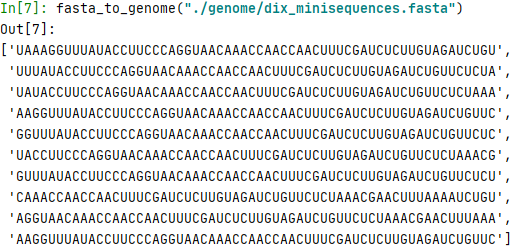
\includegraphics[scale = 0.85]{Images/Stats/app_fasta_to_genome.PNG}
        \caption{Application de la fonction \texttt{fasta\_to\_genome}}
        \label{appfasta}
    \end{figure}
% \texttt{In[7]: fasta\_to\_genome("./genome/dix\_minisequences.fasta")}\\
% \texttt{Out[7]:}\\
% \texttt{['UAAAGGUUUAUACCUUCCCAGGUAACAAACCAACCAACUUUCGAUCUCUUGUAGAUCUGU',}\\
% \texttt{~'UUUAUACCUUCCCAGGUAACAAACCAACCAACUUUCGAUCUCUUGUAGAUCUGUUCUCUA',}\\
% \texttt{~'UAUACCUUCCCAGGUAACAAACCAACCAACUUUCGAUCUCUUGUAGAUCUGUUCUCUAAA',}\\
% \texttt{~'AAGGUUUAUACCUUCCCAGGUAACAAACCAACCAACUUUCGAUCUCUUGUAGAUCUGUUC',}\\
% \texttt{~'GGUUUAUACCUUCCCAGGUAACAAACCAACCAACUUUCGAUCUCUUGUAGAUCUGUUCUC',}\\
% \texttt{~'UACCUUCCCAGGUAACAAACCAACCAACUUUCGAUCUCUUGUAGAUCUGUUCUCUAAACG',}\\
% \texttt{~'GUUUAUACCUUCCCAGGUAACAAACCAACCAACUUUCGAUCUCUUGUAGAUCUGUUCUCU',}\\
% \texttt{~'CAAACCAACCAACUUUCGAUCUCUUGUAGAUCUGUUCUCUAAACGAACUUUAAAAUCUGU',}\\
% \texttt{~'AGGUAACAAACCAACCAACUUUCGAUCUCUUGUAGAUCUGUUCUCUAAACGAACUUUAAA',}\\
% \texttt{~'AAGGUUUAUACCUUCCCAGGUAACAAACCAACCAACUUUCGAUCUCUUGUAGAUCUGUUC']}

Ensuite, il faut une fonction qui nous évalue le caractère étudié pour chaque séquence de l'échantillon. Par exemple pour la taille des séquences, nous avons la fonction \texttt{taille\_ensemble} qui prend en entrée la liste de séquences et qui renvoie la liste des tailles de chaque séquence, voir la figure~\ref{apptaille}; pour le nombre de nucléotides 'A', 'U', 'G', ou 'C', nous avons la fonction \texttt{nombre\_element\_echantillon} qui prend en entrée une liste de séquences et une base d'éléments\footnote{dans notre cas ce sont les nucléotides ou les acides aminés} qui calcule le nombre d'apparition de chaque élément de la base \footnote{nos nucléotides ou acides aminés}, voir figure~\ref{appnbelech} (en faisant appelle à la fonction \texttt{nombre\_elements}, celle-ci prend une chaîne de caractère en entrée et une base, et met dans un dictionnaire l'occurence de chaque nucléotide). Le résultat de \texttt{nombre\_element\_echantillon} est mis dans un dictionnaire sous forme de liste de la même taille que l'échantillon pour chaque élément (nucléotide ou acide aminé).
    \begin{figure}[!h]
        \centering
        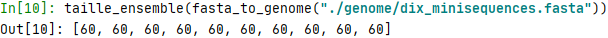
\includegraphics[scale = 0.85]{Images/Stats/app_taille_ensemble.PNG}
        \caption{Application de la fonction \texttt{taille\_ensemble}}
        \label{apptaille}
    \end{figure}
    \begin{figure}[!h]
        \centering
        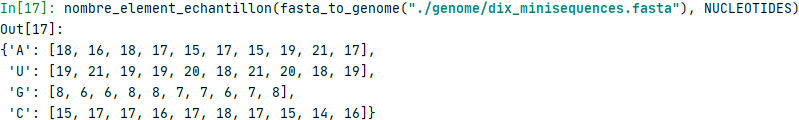
\includegraphics[scale = 0.85]{Images/Stats/app_nombre_element_echantillon.PNG}
        \caption{Application de la fonction \texttt{nombre\_element\_echantillon}}
        \label{appnbelech}
    \end{figure}

De cette manière, sur les résultats de ces fonctions (éventuellement, en sortant la liste des dictionnaires), on peut appliquer nos fonctions générales d'analyse statistique. Par exemple la fonction \texttt{moyenne} comme le montre la figure~\ref{appmoy}.
    \begin{figure}[!h]
        \centering
        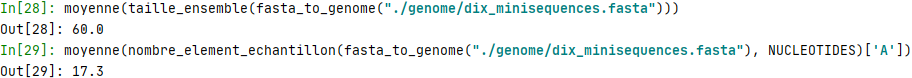
\includegraphics[scale = 0.8]{Images/Stats/app_moyenne.PNG}
        \caption{Application de la fonction \texttt{moyenne}}
        \label{appmoy}
    \end{figure}

Cependant pour alléger nos codes\footnote{afin d'éviter des structures répétitives} et réduire l'écriture d'appel à nos fonctions, nous avons introduit une fonction \texttt{call\_stats} qui prend en entrée la fonction statistique que nous voulons appliquer, l'échantillon\footnote{la liste de séquences du génome} à laquelle nous voulons appliquer la fonction statistique, la base sur laquelle nous évaluons (\texttt{NUCLEOTIDES}\footnote{est la base des nucléotides}, \texttt{AMINO\_ACIDS}\footnote{est la base des acides aminés}), et éventuellement un argument supplémentaire\footnote{pour le calcul de quartile}. La fonction \texttt{call\_stats} utilise les fonctions \texttt{nombre\_element\_echantillon} et \texttt{call\_stats\_on\_echantillon} qui font respectivement le travail de comptage\footnote{en sauvegardant la liste de valeurs dans un dictionnaire comme vu en figure~\ref{appnbelech}} et d'application de la fonction d'analyse statistique qui prend chaque élément du dictionnaire pour lui appliquer la fonction statistique donnée en entrée, la figure~\ref{appcallstats} montre une application de la fonction \texttt{call\_stats}.
    \begin{figure}[!h]
        \centering
        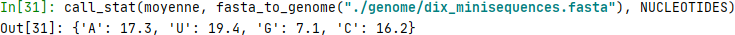
\includegraphics[scale = 0.85]{Images/Stats/app_call_stats.PNG}
        \caption{Application de la fonction \texttt{call\_stats}}
        \label{appcallstats}
    \end{figure}

La même fonction pour les statistiques sur la taille du génome a été écrite, elle s'appelle \texttt{call\_stats\_taille\_genome}, celle-ci prend en entrée une fonction statistique, une liste de séquences et éventuellement un argument supplémentaire, elle appelle la fonction \texttt{taille\_ensemble} pour donner dans une liste la taille de chaque génome de l'échantillon et c'est sur cette liste qu'elle applique la fonction statistique, la figure~\ref{appcallstatstaille} montre ceci.
    \begin{figure}[!h]
        \centering
        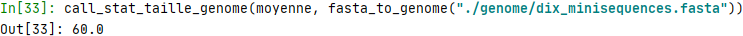
\includegraphics[scale = 0.85]{Images/Stats/app_call_stats_taille_genome.PNG}
        \caption{Application de la fonction \texttt{call\_stats\_taille\_genome}}
        \label{appcallstatstaille}
    \end{figure}



\subsubsection{Applications des fonctions statistiques sur des échantillons}
Toutefois, les fonctions \texttt{perform\_all\_stats} et \texttt{perform\_all\_stats\_taille} ont été introduites pour appeler toutes les fonctions d'analyse statistique en une fois, cela réduit les lignes de codes à écrire pour les appels et répond aux premier objectif du projet qui est de décrire en utilisant la statistique descriptive le génome du SARS-CoV2.

La fonction \texttt{perform\_all\_stats} prend en entrée une liste de séquences et une base d'élément (nucléotides par exemple), elle appelle toutes les fonctions statistiques\footnote{en utilisant \texttt{nombre\_element\_echantillon} et \texttt{call\_stat\_on\_echantillon}} et renvoie dans un dictionnaire la valeur statistique de chaque élément. Sur la figure~\ref{appnucl10000seq}, les résultats de deux applications de la fonction \texttt{perform\_all\_stats} sur deux échantillons de dix mille séquences de nucléotides de période différente\footnote{l'une sont des séquences de janvier 2020 à août 2020, et l'autre sont des séquences d'octobre à novembre 2020} sont mis en évidence.
    \begin{figure}[!h]
        \centering
        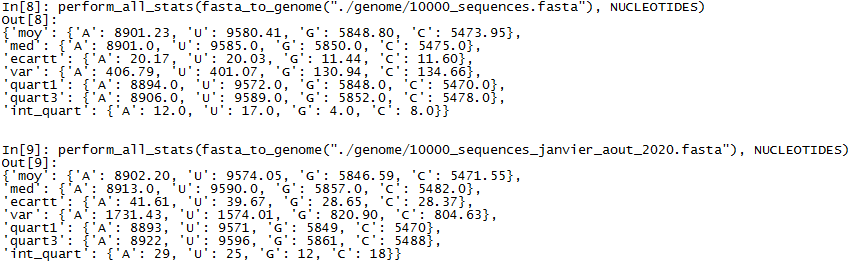
\includegraphics[scale = 0.75]{Images/Stats/app_10000_seq.PNG}
        \caption{Application de la fonction \texttt{perform\_all\_stats} sur deux échantillons de 10000 séquences}
        \label{appnucl10000seq}
    \end{figure}\\

\newpage
    
Les résultats des deux applications sur les deux échantillons diffèrent très peu. En effet, nous avons à peu près en moyenne 8901 (avec plus ou moins 20 d'écart) nucléotides A, 9580 (avec plus ou moins 20 d'écart)  nucléotides U, 5849 (avec plus ou moins 11 d'écart)  nucléotides G et 5474 (avec plus ou moins 11 d'écart) nucléotides C. Les médianes sont très proches des moyennes, ceci nous laisse croire que la répartition est plutôt symétrique, l'écart interquartile est assez petit, donc nous supposons que les valeurs sont assez regroupées autour de la médiane. De plus l'écart-type de chaque nucléotide est acceptable, il ne dépasse pas 20 pour l'échantillon d'octobre à novembre, mais celui de janvier à août est plus important (environ le double). Cette différence peut s'expliquer par le fait que l'échantillon de janvier à août est d'une période plus large que celui d'octobre à novembre, le virus a pu muter beaucoup plus de fois, produisant des séquences qui s'écartent de plus en plus de la moyenne. Un exemple graphique sur le nucléotide G est illustré par la figure~\ref{graph:nuclG}, et un exemple d'application de la fonction \texttt{proportions} est montré sur la figure~\ref{graph:propnucl}.

    \begin{figure}[!h]
        \centering
        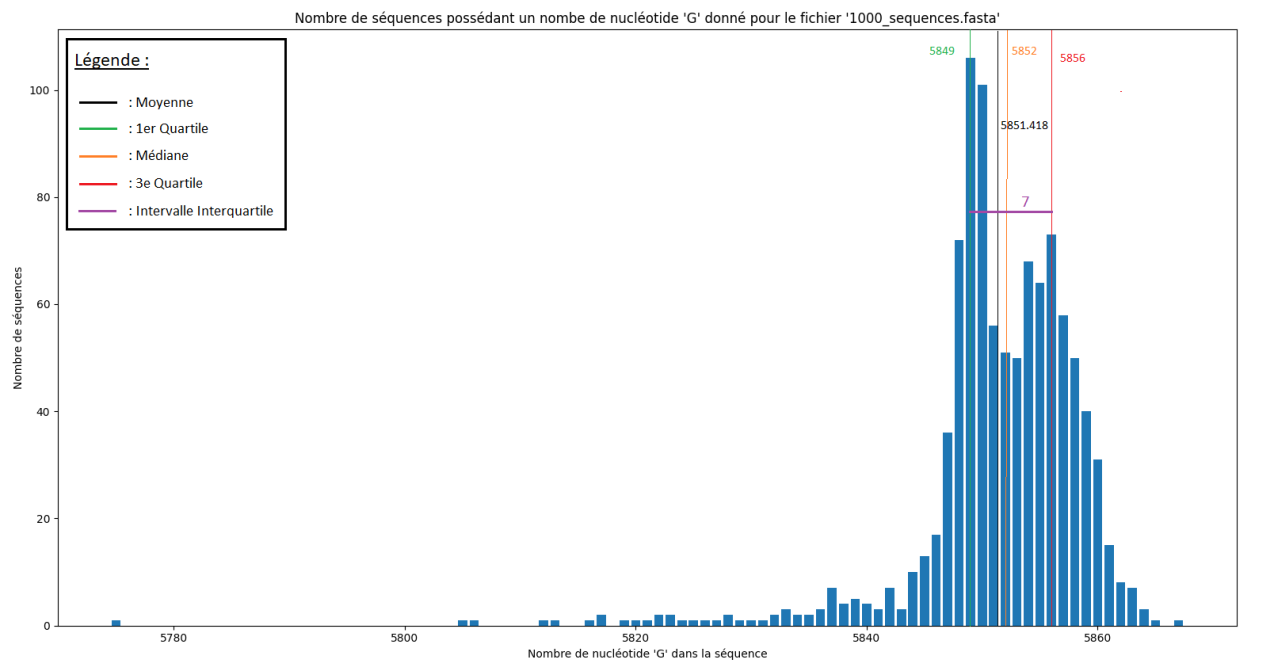
\includegraphics[scale = 0.4]{Images/Stats/Nucléotides/graphe_nucl_G.png}
        \caption{La répartition des nombres de nucléotides G des séquences d'un échantillon de 1000}      \label{graph:nuclG}
    \end{figure}
    \begin{figure}[!h]
        \centering
        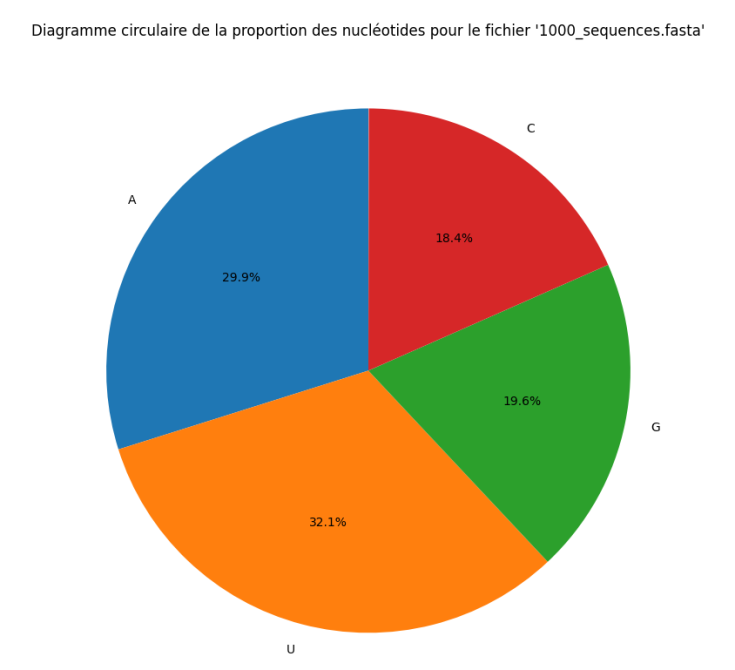
\includegraphics[scale = 0.43]{Images/Stats/Nucléotides/graphe_props_nucl.png}
        \caption{Proportions des nucléotides dans un échantillon de 1000}      \label{graph:propnucl}
    \end{figure}

La fonction \texttt{perform\_all\_stats\_taille} prend en entrée une liste de séquences\footnote{un échantillon}, elle applique les fonctions statistiques en utilisant la fonction \texttt{call\_stat\_taille\_genome}, et renvoie dans un dictionnaire les valeurs statistiques sur l'échantillon sur la taille du génome. Sur la figure~\ref{apptaille10000seq}, les résultats de deux applications de la fonction \texttt{perform\_all\_stats} sur deux échantillons de dix mille séquences de nucléotides de périodes différentes\footnote{l'une sont des séquences de janvier à août 2020, et l'autre sont des séquences d'octobre à novembre 2020} sont mis en évidence.
    \begin{figure}[!h]
        \centering
        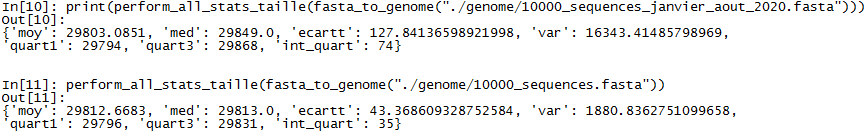
\includegraphics[scale = 0.8]{Images/Stats/app_10000_seq_taille.PNG}
        \caption{Application de la fonction \texttt{perform\_all\_stats\_taille} sur deux échantillons de 10000 séquences}
        \label{apptaille10000seq}
    \end{figure}
    
De même que précédemment, les résultats des deux applications sur les deux échantillons diffèrent très peu. Nous avons en moyenne 29812 (avec plus ou moins 43 d'écart) nucléotides pour chaque séquence du génome. On retrouve les mêmes conclusions, la moyenne est assez proche de la médiane, l'écart interquartile n'est pas très grand, les valeurs sont plutôt symétriques et regroupées autour de la médiane. L'écart-type est plutôt petit par rapport à la taille des séquences, cependant pour l'échantillon de janvier à août, il est presque trois fois plus grand que celui d'octobre à novembre. Pareillement, cette différence peut s'expliquer par le fait que l'échantillon de janvier à août est d'une période plus large que celui d'octobre à novembre, le virus a pu muter beaucoup plus de fois, produisant des séquences qui s'écartent de plus en plus de la moyenne.

Par ailleurs, une représentation graphique de l'application sur un échantillon de 1000 séquences a été réalisé, voir figure~\ref{graph:taillenucl} et en comparaison avec les résultats précédents, les différences sont assez petites.
    \begin{figure}[!h]
        \centering
        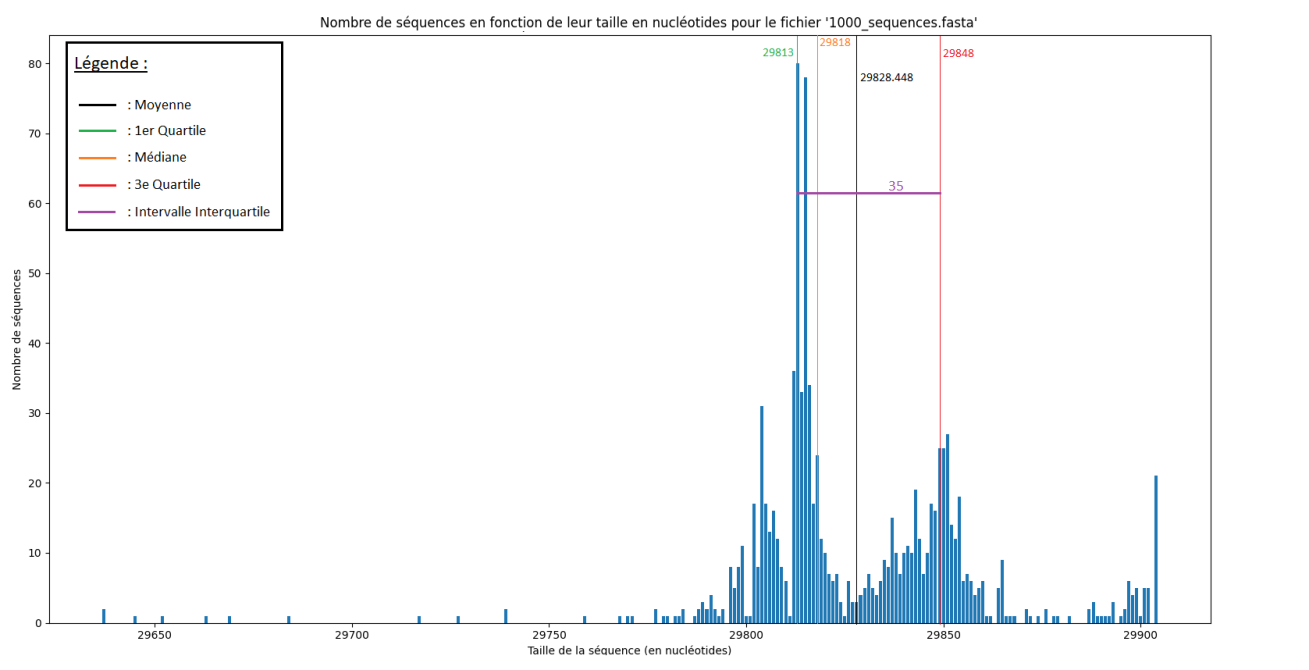
\includegraphics[scale = 0.4]{Images/Stats/Nucléotides/graphe_taille_nucl.png}
        \caption{La répartition de la taille des séquences de nucléotides dans un échantillon de 1000}      \label{graph:taillenucl}
    \end{figure}



\subsection{La fonction \texttt{codons}}

Le but de cette partie est d'écrire une fonction \texttt{codons} qui permet de générer les séquences d'acides aminés. La fonction doit prendre en paramètre une liste d'ARNm et renvoie la liste de la séquence d'acides aminés. \\

Pour l'implémentation de la fonction, les codons et leur acide aminé correspondant ont été ajoutés comme une constante globale dans le fichier \texttt{globals.py} sous forme d'un dictionnaire  \texttt{CODONS\_TO\_AMINO\_ACIDS}. La structure du dictionnaire a été choisie pour sa facilité d'appel et sa structure non-ordonnée. \\

\label{subsec:imp_codons}
Aprés de multiples documentations, un problème de traduction entre les codons START et STOP a été pris en compte. Donc une fonction \texttt{start\_to\_stop} a été implémentée pour séléctionner les séquences de l'ARNm sur lesquelles on va appliquer la fonction \texttt{codons}. Ces séquences sont retournées sous forme d'une liste de chaînes de caractères. \

Toutefois, en appliquant la fonction sur les séquences du génome fournies par le site~: 
\textsl{National Center for Biology Information (NCBI)}, un nouveau problème a été rencontré. Il y avait des codes IUPAC dans les fichiers FASTA autres que les quatres de base (A, G, C et U). Le problème c'est que ces codes, comme indiqué dans la table~\ref{fig:table des codes IUPAC}, page~\pageref{fig:table des codes IUPAC}, peuvent avoir plusieurs traductions, comme ar exemple, le code N qui fait référence à n'importe quel nucléotide. On a donc pris en considération le code R (A ou G) dans la liste des codons STOP (UGA, UAA, UAG, UAR). Sachant que le codon UAR couvre les deux cas (UAA et UAG). 
Pour les autres codes plusieurs solutions ont été prensées~:
\begin{itemize}
\item L'implémentation d'une fonction \texttt{random} qui retourne aléatoirement le nucléotide~: cette solution a été rejetée puisque dans des sequences il peut y avoir, par exemple, une succession de plusieurs N. Donc, cela serait comme si on génèrait toute une sous-séquence aléatoirement et les résultats seront erronées.
\item L'étude de tous les cas, c'est-à-dire, à chaque code on fait une séquence pour chaque nucléotide possible. Cette solution aussi a été rejetée car cela serait très lourd en terme de mémoire et pour chaque séquence on aurait plus d'une centaine de séquences\footnote{L'explosion combinatoire}.
\item L'implémentation d'une fonction \texttt{try\_AUGC} qui teste s'il y a un code autre que les nucléotides. Puis, on ignore tout codon contenant un code différent de (A, G, U, C et R). C'est la solution qui a été adaptée au final. 
\end{itemize}

Finalement, la fonction \texttt{codons}, voir figure~\ref{fig: fctCodons}, prend en paramètre une chaîne de caractères ou une liste d'ARNm et renvoie une liste des séquences d'acides aminés qui correspond à la traduction de chaque séquence entre les codons START et STOP tout en ignorant le problème des codes IUPAC. 

     \begin{figure}[!h]
        \centering
        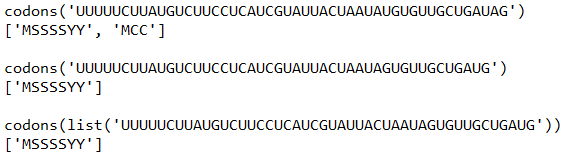
\includegraphics[scale = 1.2]{Images/Codons/app_codons.png}
        \caption{Application de la fonction \texttt{codons} }
        \label{fig: fctCodons}
    \end{figure}

Mais, on a tout de même gardé la première version de \texttt{codons}, nommée \texttt{codons\_v2}, voir figure~\ref{fig: fctCodonsV2}, qui ne tient pas compte ni du problème de START et STOP ni celui des codes IUPAC autres que les basiques (A, G, C et U). Elle prend simplement en paramètre la liste d'ARNm et renvoie une chaîne des acides aminés. 

     \begin{figure}[!h]
        \centering
        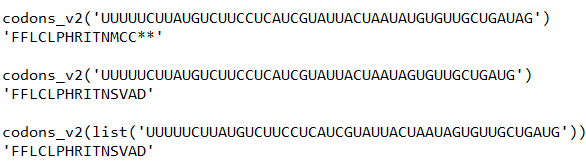
\includegraphics[scale = 1.2]{Images/Codons/app_codons_v2.png}
        \caption{Application de la fonction \texttt{codons\_v2} }
        \label{fig: fctCodonsV2}
    \end{figure}

Dû à l'ambiguïté du sujet, une troisième version de la fonction nommée \texttt{codons\_v3} à été implémentée, voir figure~\ref{fig: fctCodonsV3}, qui prend en paramètre l'ARNm  et renvoie le même résultat que \texttt{codons} mais sous forme d'une chaine de caractères. Cette version est utile pour les applications des analyses statistiques. Par conséquent, une fonction \texttt{codons\_echantillon} a été implémentée, prennant en paramètre un échantillon du génome (plusieurs séquences d'ARNm) et renvoyant la liste des séquences d'acides aminés qui convient.

     \begin{figure}[!h]
        \centering
        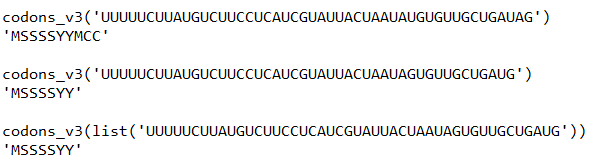
\includegraphics[scale = 1.2]{Images/Codons/app_codons_v3.png}
        \caption{Application de la fonction \texttt{codons\_v3} }
        \label{fig: fctCodonsV3}
    \end{figure}



\subsubsection{Étude de l'algorithme}
L'algorithme de la fonction \texttt{codons} s'exécute en complexité linéaire. En effet, la fonction \texttt{start\_to\_stop} s'exécute en complexite linéaire. Pour chaque séquence entre START et STOP, de taille inférieure ou égale à la séquence d'ARNm initiale, on la parcourt avec un pas de trois.

\subsubsection{Applications et interprétations}
Nous avons appliqué les fonctions de l'analyse statistique descriptive sur les séquences d'acides aminés comme indiqué sur les figures~\ref{fig: echantillonJanvAvril} et~\ref{fig: echantillonOctNov} pour la fonction \texttt{perform\_all\_stats}.\\
Un exemple graphique sur l'acide aminé L est illustré par la figure~\ref{graph:acL}.

     \begin{figure}[!h]
        \centering
        \includegraphics[scale = 0.75]{Images/Codons/app_codon_acide_aminé22.png}
        \caption{Échantillon de Janvier à Avril 2020}
        \label{fig: echantillonJanvAvril}
    \end{figure}
    
     \begin{figure}[!h]
        \centering
        \includegraphics[scale = 0.75]{Images/Codons/app_codon_acide_aminé1.png}
        \caption{Échantillon d'Octobre à Novembre 2020}
        \label{fig: echantillonOctNov}
    \end{figure}

 
    \begin{figure}[!h]
        \centering
        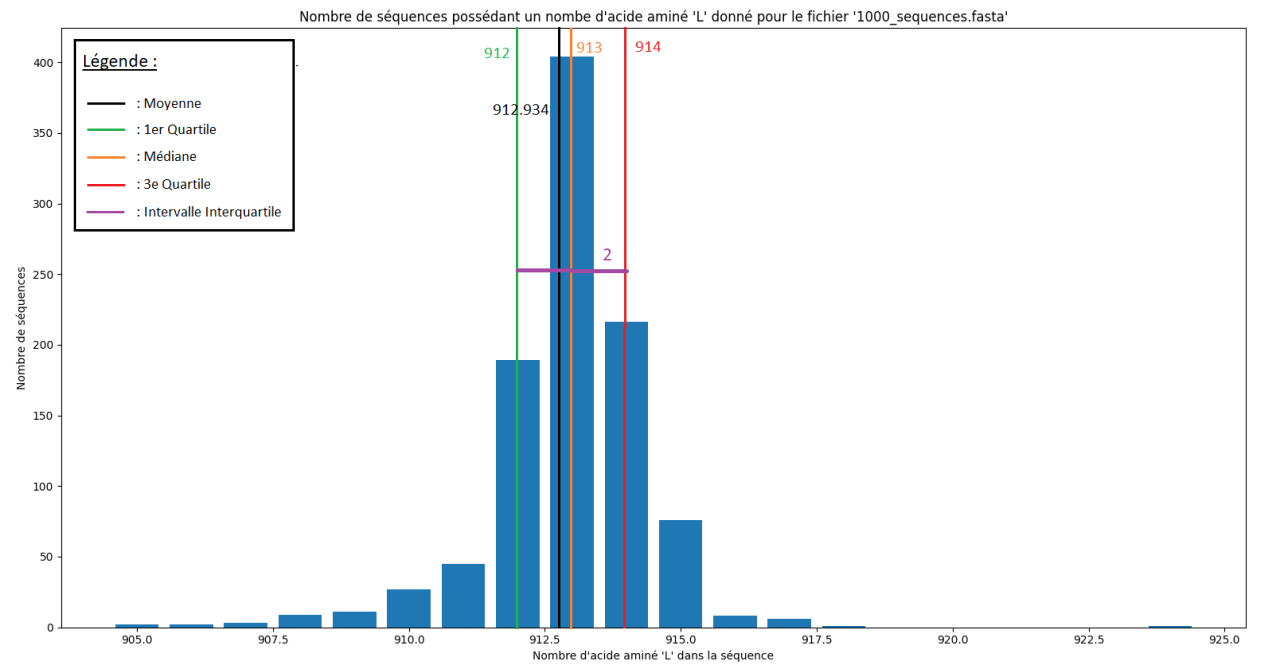
\includegraphics[scale = 0.7]{Images/Stats/Codons/graphe_acide_L.png}
        \caption{Nombres d'acides aminés L des séquences d'un échantillon de 1000 séquences}      \label{graph:acL}
    \end{figure}
    
\newpage

On remarque que pour deux échantillons de périodes différentes, les résultats des analyses statistiques sont comparables. \\
Sur la figure~\ref{graph:propac}, on trouve un exemple d'application de la fonction \texttt{perform\_all\_stats\_proportion}.

    \begin{figure}[!h]
        \centering
        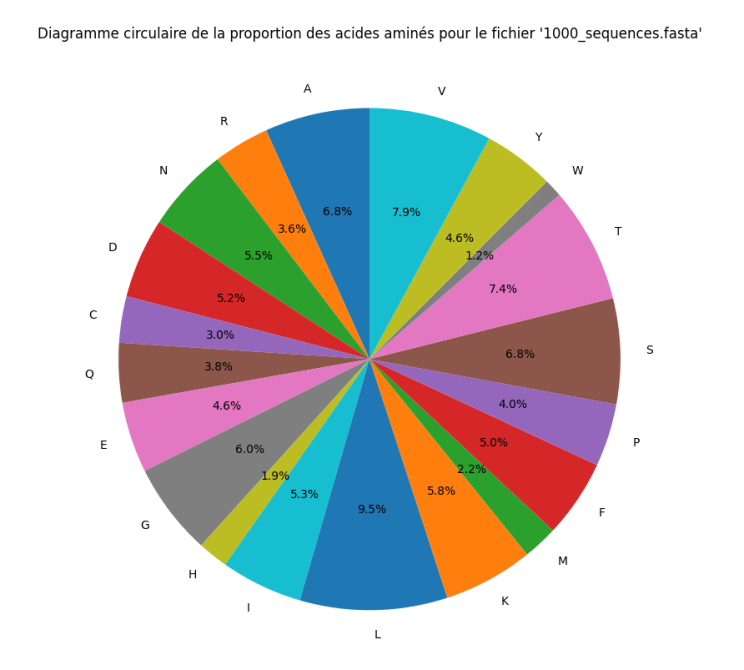
\includegraphics[scale = 0.5]{Images/Stats/Codons/graphe_props_acide.png}
        \caption{Proportions des acides aminés dans un échantillon de 1000 séquences}     
        \label{graph:propac}
    \end{figure}

\newpage

Nous avons appliqué aussi la fonction \texttt{perform\_all\_stats\_taille}. Sur les deux figures~\ref{fig: appcodonstaille1000} et~\ref{fig: appcodonstaille10000}, les résultats de l'application de la fonction sur deux échantillons~: l'un de mille séquences d'acides aminés et l'autre de dix milles séquences d'acides aminés.\\

    \begin{figure}[!h]
        \centering
        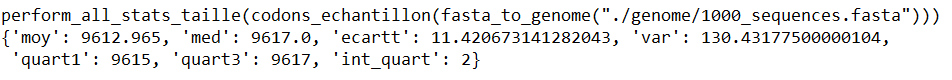
\includegraphics[scale = 0.9]{Images/Codons/app_codons_taille1000.png}
        \caption{Application de la fonction \texttt{perform\_all\_stats\_taille} sur 1000 séquences d'acides aminés }
        \label{fig: appcodonstaille1000}
    \end{figure}


     \begin{figure}[!h]
        \centering
        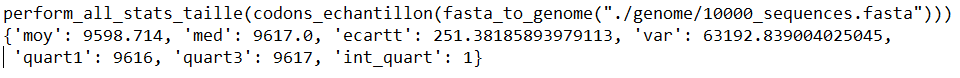
\includegraphics[scale = 0.9]{Images/Codons/app_codons_taille10000.png}
        \caption{Application de la fonction \texttt{perform\_all\_stats\_taille} sur 10000 séquences d'acides aminés}
        \label{fig: appcodonstaille10000}
    \end{figure}

\newpage 

La figure~\ref{graph:taille} illustre l'histogramme de nombre de séqunece en fonction de leur taille en acides aminés.

    \begin{figure}[!h]
        \centering
        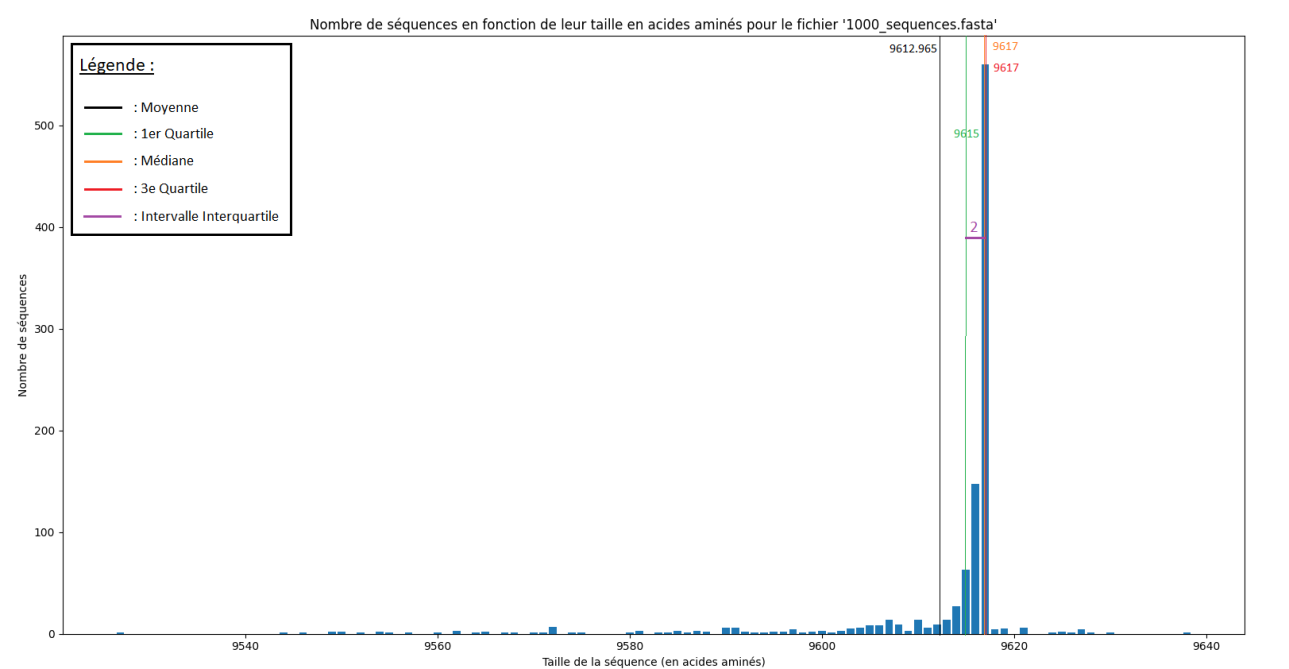
\includegraphics[scale = 0.4]{Images/Stats/Codons/graphe_taille_acide.png}
        \caption{Nombre de séquences en fonction de leur taille en acides aminés dans un échantillon de 1000}      
        \label{graph:taille}
    \end{figure}
    
    
    
\subsection{La distance de Levenshtein}
\label{subsec:lev}

Nous avons implémenté trois algorithmes pour le calcul de la distance de Levenstein : une version récursive classique \texttt{lev\_rec}, une version en programmation dynamique récursive \texttt{lev\_dp} et une version en programmation dynamique itérative  \texttt{lev}, qui est nôtre version privilégiée. Toutes les trois prennent en paramèrtre deux chaines de caractères, $seq1$ et $seq2$, et renvoient un entier positif correspondant à la distance de Levenstein entre les deux chaînes de caractères saisies en entrée.

\subsubsection{\texttt{lev\_rec}}
La fonction \texttt{lev\_rec} est une version récursive du calcul de la distance de Levenstein qui ne fait pas appel à la programmation dynamique.
L'algorithme est assez simple, on distingue quatre cas.\\

On a deux cas de base : si la longueur de \texttt{seq1} est égale à $0$ ou si la longueur de \texttt{seq2} est égale à $0$, alors on renvoie la longueur de \texttt{seq2} ou la longueur de \texttt{seq1} respectivement. C'est normal puisque si un des mots est vide, la distance de Levenstein entre les deux correspond à la longueur du second mot.\\

Troisième cas : si la première lettre de \texttt{seq1} est la même que la première lettre de \texttt{seq2}, alors on fait un appel récursif de \texttt{lev\_rec} en prenant en paramètre \texttt{seq1} et \texttt{seq2} privées de leur première lettre. En effet, si ces deux premières lettres sont identiques, les enlever des deux mots ne change pas la distance de levenstein entre les deux.\\

\newpage

Quatrième cas : si ces deux premières lettres ne sont pas identiques, on incrémente la distance de Levenstein en ajoutant 1 au minimum des appels récursifs de \texttt{lev\_rec} avec \texttt{seq1} privée de sa première lettre, \texttt{lev\_rec} avec \texttt{seq2} privée de sa première lettre et \texttt{lev\_rec} avec \texttt{seq1} et \texttt{seq2} privées de leur première lettre. Ceci correspond à prendre en compte le mismatch ($+1$) et à y ajouter la distance de Levenstein minimale entre les deux chaînes de caractères dont l'une des deux ou les deux se voient privées de leur première lettre. Nous sommes obligés de prendre le minimum entre ces trois cas car ils permettent récursivement de couvrir toutes les possibilités.\\

Au final, la fonction renvoie bien la distance de Levenstein entre les deux chaînes de caractères $seq1$ et $seq2$. Cependant, l'obligation de multiplier les appels récursifs mène à une explosion combinatoire pour de très longues chaînes de caractères, ce qui peut mener à une erreur de "Stack overflow". En effet, dans le pire des cas où les chaînes de caractères sont complètement différentes, cet algorithme effectue trois appels récursifs et le fait en réduisant altrenativement la taille de \texttt{seq1} et \texttt{seq2}, pour un total de $m+n-1$ fois (car on s'arrête lorsqu'une des chaînes de caractères est vide). Ainsi, la complexité de cet algorithme est majorée en $O(3^{n+m})$, et c'est pourquoi cette solution n'est pas fiable pour l'étude de génomes, dont la taille est trop importante.

\subsubsection{\texttt{lev\_dp}}
La fonction \texttt{lev\_dp} est une version récursive du calcul de la distance de Levenstein qui fait appel à la programmation dynamique.

Puisque l'on utilise la programmation dynamique, l'algorithme commence par créer une matrice de dimension $(n+1)\times (m+1)$ comme décrit dans l'état de l'art. Ici, nous la remplissons de -1, ce qui permet à l'algorithme de savoir si une case a déjà  été calculée ou pas.\\
Ainsi, on distingue cinq cas, dont trois cas de base:
\begin{itemize}
    \item Premier cas (cas de base): Si la dernière case de la matrice \texttt{dp[n+1][m+1]} n'est pas égale à -1, cela veut dire qu'elle a été calculée. Puisque cette case correspond à la distance de Levenstein recherchée, on renvoie cette valeur.
    \item Deuxième cas (cas de base): Si la longueur de \texttt{seq1} est nulle, cela veut dire que la distance de Levenstein correspond à la longueur de \texttt{seq2}, donc on renvoie cette valeur.
    \item Troisième cas (cas de base): Idem que pour le deuxième cas mais en inversant \texttt{seq1} et \texttt{seq2}.
    \item Quatrième cas : Si les premières lettres de \texttt{seq1} et \texttt{seq2} sont identiques, alors on attribue à \texttt{dp[n+1][m+1]} la valeur de l'appel récursif de la fonction auxiliaire \texttt{lambda\_lev\_rec} avec en paramètre les chaînes de caractères \texttt{seq1} et \texttt{seq2} privées de leur premières lettres. Au fil des appels récursifs, on tombera sur un des cas de base et ainsi \texttt{lambda\_lev\_rec} prendra bien la valeur de la distance de Levenstein calculée. On retourne cette valeur.
    \item Cinquième cas : Si aucun des cas précédents n'est vérifié, alors c'est que l'on doit effectuer une addition, une suppression ou une substitution. On attribue donc à la dernière case de la \texttt{matrice dp[n+1][m+1]} la valeur 1 + la valeur minimale entre les appels récursifs de la fonction auxiliaire \texttt{lambda\_lev\_rec} avec en paramètre \texttt{seq1} et/ou \texttt{seq2} privées de leur premières lettres ainsi que la matrice dp, ce qui permet de couvrir tous les cas. Au fil des appels récursifs, on tombera sur un des cas de base et ainsi \texttt{lambda\_lev\_rec} prendra bien la valeur de la distance de Levenstein calculée. On retourne cette valeur.
\end{itemize}
Ainsi, on calcule récursivement la distance de Levenstein mais en utilisant une matrice "dp" qui fait office de "sauvegarde" des données déjà calculées. Ainsi, dans le pire cas on n'effectue que $(n+1)\times (m+1) = n\times m +n +m +1$ opérations au maximum, ce qui est majoré en $O(n\times m)$. Ainsi, cette fonction est théoriquement largement plus efficace que \texttt{lev\_rec} pour des chaînes de caractères plus longues. Cependant, il existe une solution encore meilleure, présentée ci-après. 

\subsubsection{\texttt{lev}}
La fonction \texttt{lev} est une version itérative du calcul de la distance de Levenstein qui fait aussi appel à la programmation dynamique. Son fonctionnement est le plus simple parmis les trois versions proposées, et aussi la plus efficace. Notez que le déroulement ne suit pas exactement celui énoncé dans l'état de l'art. Ici, l'étape d'initialisation est directement incorporée dans l'étape de remplissage, cela a quelques conséquences sur les indices de la boucle.\\

La fonction commence par créer une matrice nommée "dp" de dimension $(m+1)\times (n+1)$ remplie de -1. Ici, la valeur -1 n'a aucune importance.
On rentre ensuite dans la double boucle parcourant chaque case de la matrice "dp" et on distingue quatre cas :
\begin{itemize}
    \item Premier et deuxième cas : Si i = 0, alors \texttt{dp[i][j]} prend la valeur j et sinon si j = 0 alors \texttt{dp[i][j]} prend la valeur i (ce qui correspond à l'étape d'initialisation).
    \item Troisième cas : Si les deux cas précédents ne sont pas vérifiés et si \texttt{seq1[i - 1] = seq2[j - 1]}, alors \texttt{dp[i][j]} prend la valeur \texttt{dp[i-1][j-1]}. Ce cas correspond à un match mais comparé à l'état de l'art, on compare les lettres \texttt{seq1[i-1]} avec \texttt{seq2[j-1]} au lieu de comparer \texttt{seq1[i]]} avec \texttt{seq2[j]}. En effet, la matrice "dp" doit forcément être de dimension $(m+1)\times (n+1)$ pour inclure le "gap" devant les mots, et donc $i$ et $j$ varient de $1$ à $n+1$ et $m+1$. Or \texttt{seq1} et \texttt{seq2} ne sont que de longueur $n$ et $m$ puisque nous n'avons pas ajouté artificiellement le gap devant les chaînes de caractères. Nous sommes donc obligés de soustraire $1$ aux indices \texttt{i} et \texttt{j} dans \texttt{seq1[i-1]} et \texttt{seq2[j-1]}. En somme, cela revient à mettre les gaps à la fin des mots.
    \item Quatrième cas : Si aucun des cas précédents ne soient vérifiés, alors \texttt{dp[i][j]} prend la valeur $1 +$ le minimum entre les cases à gauche, au dessus et en diagonale en haut et à gauche (\texttt{dp[i-1][j], dp[i][j-1], dp[i-1][j-1]})
\end{itemize} 

Au final, on renvoie \texttt{dp[n][m]} qui est notre distance de Levenstein. Le fait d'implémenter une matrice "dp" de dimension $(m+1)\times (n+1)$ permet de réduire la complexité en $O(m\times n)$. En effet, quelque soient les longueurs des chaînes de caractères, l'algorithme effectue $(m+1)\times (n+1) = m\times n + m + n +1$ opérations, ce qui est majoré en $O(m\times n)$.
De plus, d'après les graphiques de performance, cette version est plus rapide que la version récursive en programmation dynamique \texttt{lev\_dp}, bien qu'elle soit elle aussi majorée en $O(m\times n)$. Nous pensons que cela est du à un coût supplémentaire par rapport à la gestion de la pile due aux appels récursifs successifs de la fonction.\\
C'est pourquoi \texttt{lev} est notre fonction la plus efficace pour le calcul de la distance de Levanstein.


\subsubsection{Applications et interprétation}
La fonction \texttt{meme\_taille} prend en argument deux listes de chaînes de caractères de tailles différentes et qui retourne deux listes de la même taille en ajoutant des chaînes vides.
La fonction \texttt{affiche\_res} a été implémentée pour l'affichage du résultat. Elle prend en argument les deux séquences d'acides aminés\footnote{obtenues par l'application de la fonction \texttt{codons} sur deux ARNm de la base NCBI.}. \\
Différentes applications ont été faites en comparant à chaque fois les séquences de codons selon les critères de la période et du lieu: 
\begin{itemize}[label=\textbullet]%, font=\large \color{green}]
    \item Différentes périodes et différents lieu : 
    \begin{itemize}
        \item La comparaison est entre une première séquence prise de la Chine, la séquence "originelle" de Wuhan en janvier 2020, et une deuxième séquence prise des Etats Unis en décembre 2020. 
        Comme indiqué sur la figure~\ref{fig: MatriceUSAchine}, on remarque que le début des séquences est identiques mais à partir d'un endroit il y a beaucoup de changement (les mutations) au milieu et à la fin des séquences.
        
    \begin{figure}[!h]
        \centering
        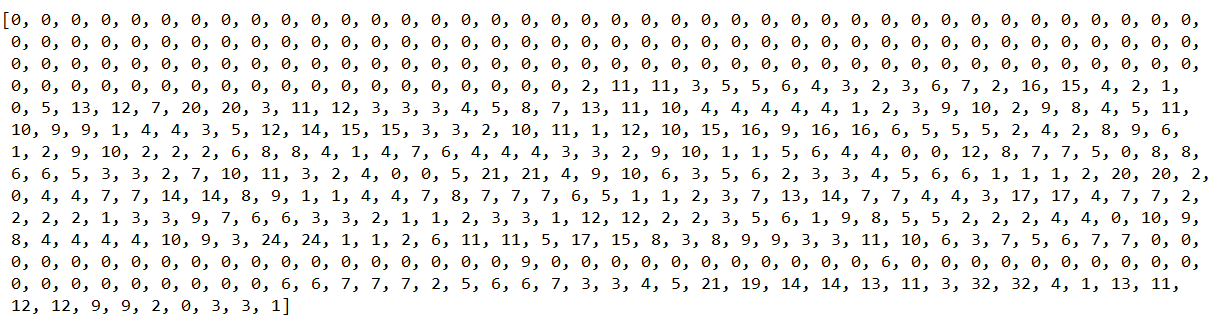
\includegraphics[scale = 0.65]{Images/Levenstein/USAChina DIFFERENTE PERIODE DIFFERENT LIEU.png}
        \caption{Application de la fonction \texttt{lev} sur les séquences des Etats-Unis en décembre 2020 et de Chine en janvier 2020 }
        \label{fig: MatriceUSAchine}
    \end{figure}
    
        \item Une comparaison entre une première séquence prise du Brésil en Mars 2020 et une deuxième séquence prise des États-Unis en décembre 2020 est montrée sur la figure~\ref{fig: MatriceUSABrésil}. Les deux séquences sont presque identiques, il n'y a que deux ou trois changements.\\
        
    \begin{figure}[!h]
        \centering
        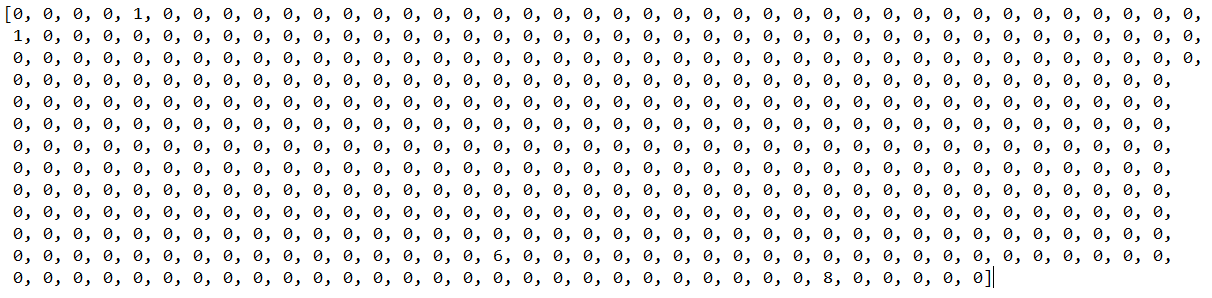
\includegraphics[scale = 0.65]{Images/Levenstein/USABrezil DIFFERENTE PERIODE DIFFERENT LIEU.png}
        \caption{Application de la fonction \texttt{lev} sur les séquences  des Etats-Unis en décembre 2020 et du Brésil en Mars 2020}
        \label{fig: MatriceUSABrésil}
    \end{figure}
    
    \end{itemize}
    \item Même période :
    \begin{itemize}
        \item Une comparaison entre deux séquences proches en période, de Belgique et d'Allemagne en décembre 2020\footnote{et proche en lieu aussi}. Les résultats sont représentés sur la figure~\ref{fig: MatricebelgiumGerman}, les séquences diffèrent très peu.
        \item Une comparaison entre deux séquences de même période, mais de de lieux éloignés, des Etats-Unis et de la Tunisie en décembre 2020, a été fait. Elles diffèrent peu également.
        
    \begin{figure}[!h]
        \centering
        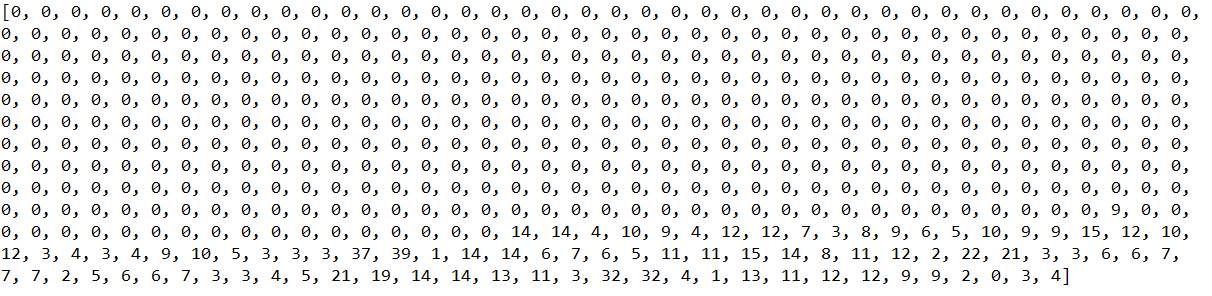
\includegraphics[scale = 0.65]{Images/Levenstein/belgium_germany MEME PERIODE.png}
        \caption{Application de la fonction \texttt{lev} sur les séquences de Belgique et d’Allemagne en décembre 2020}
        \label{fig: MatricebelgiumGerman}
    \end{figure}
    \end{itemize}
    \item Même lieu :
    \begin{itemize}
        \item Une comparaison entre deux séquences de même lieu (la Chine) et de périodes différentes. L'une en janvier 2020 et l'autre en mars 2020 montre que
        les séquences sont identiques avec juste un changement dans la dernière partie (voir figure~\ref{fig: MatriceChine}).
        
    \begin{figure}[!h]
        \centering
        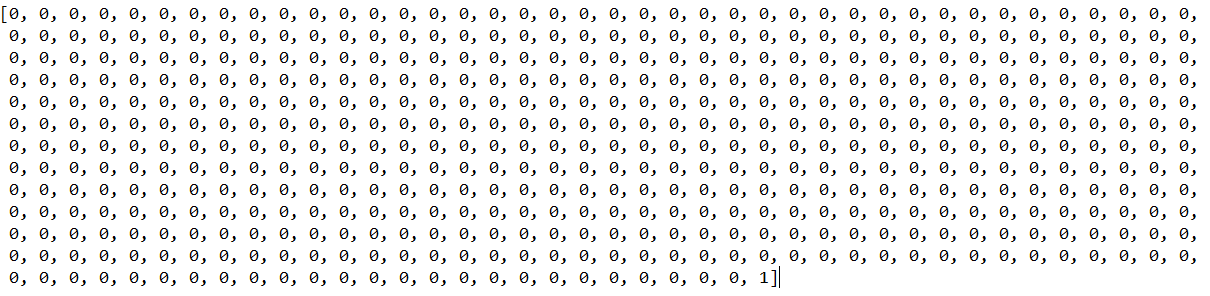
\includegraphics[scale = 0.65]{Images/Levenstein/China_diffperiode MEME LIEU.png}
        \caption{Application de la fonction \texttt{lev} sur deux séquences différentes de la Chine en mars 2020}
        \label{fig: MatriceChine}
    \end{figure}
        \item Une comparaison entre deux séquences de même lieu (les Etats-Unis Californie) et de périodes différentes décrit que les séquences sont presque identiques au début avec des changements sur les dernières séquences d'acides aminés.
    \end{itemize}
    \item Même période et même lieu :
    \begin{itemize}
        \item Deux séquences (choisies au hasard) de même lieu (la Chine) et de mêmes périodes (mars 2020) sont presque identiques.
        \item Une comparaison entre deux séquences de même lieu (les Etats-Unis Californie) et de mêmes périodes (décembre 2020) montre qu'elles sont identiques sauf à la fin l'une est plus longue que l'autre.
    \end{itemize}
\end{itemize}
En conclusion, on peut remarquer que dans le plus part du temps la mutation s'effectue à la fin de la séquence du génome soit par changement des séquences d'acides aminés, soit par l'ajout de ces dernières (justifié par différence de taille des séquences).



\subsubsection{Pistes d'amélioration possibles}
Comme mentionné dans l'état de l'art, il serait possible d'améliorer les fonctions en y ajoutant un moyen de personnaliser les coûts d'addition, de suppression et de substitution d'un caractère. De plus, on pourrait effectuer le calcul en ne gardant que la ligne précédente plutôt que de sauvegarder tout le tableau, ce qui permetterait de gagner un peu d'espace mémoire.



\subsection{L'algorithme de Needleman-Wunsch}
\label{subsec:nw_impl} 
L'algorithme de Needleman-Wunsch doit avoir deux versions de fonctionnement (l'une qui prend la matrice de similarité \footnote{ou matrice de coût} et l'autre qui prend juste le coût du \textit{match}, \textit{mismatch} et le \textit{gap}). Afin de profiter des similitudes entre ces deux versions et dans le but d'éviter les répétitions des codes, les différents arguments ont été regroupés, aboutissant à la fin en une seule fonction polymorphe\footnote{Le comportement de la fonction change légèrement en fonction des paramètres fournis, ce qui est similaire au concept de surcharge de fonction}. Pour une telle fonction, il est nécessaire de faire des vérifications supplémentaire qui s’assurent de la correcte utilisation de la fonction et qui garantissent l’exclusivité mutuelle de ces différents arguments.

La structure des arguments est identique pour \texttt{needleman} et \texttt{needleman\_all}. Les deux premiers arguments sont respectivement la première et la deuxième séquence. Ensuite, nous passons soit une table de coûts, soit une matrice de coûts et une clé. La table \texttt{cost\_table}\footnote{table de coûts} est une liste qui contient les coûts de \textit{match}, \textit{mismatch} et le \textit{gap} (dans cet ordre). L'ensemble composé de la matrice de coûts (\texttt{cost\_matrix}) et de la clé (\texttt{key}) est mutuellement exclusive avec la \texttt{cost\_table} (soit l'un, soit l'autre). La manière dont la \texttt{cost\_matrix} est lue et interprétée dépend fortement de la clé et de sa valeur. Fondamentalement, la \texttt{cost\_matrix} est un table python avec une longueur égale à la longueur de la clé au carré en ajoutant un (le dernier élément de la table \texttt{cost\_matrix} qui est en fait le score de l'écart, le \textit{gap}). Le premier élément de la table correspond au coût entre le premier caractère de la clé et lui-même, le deuxième élément est le coût entre le premier et le deuxième caractère de la clé, et ainsi de suite. Par exemple, nous avons la table et la clé suivante~:\\ \texttt{cost\_mat = [  -1, -2, -3, -4, -5, -6, -7, -8, -9, -10  ]} 
et \texttt{key = "ABC"}\\
Alors, la matrice de coûts (de similarité) sera dans la table~\ref{tab:matcout} suivante~:\\
\begin{table}[!h]
    \centering
    \begin{tabular}{|l|c|c|c|c|}
        \hline
         & \multicolumn{4}{|c|}{Letter 2} \\
        \hline
         &   & A & B & C  \\ \cline{2-5}
         & A & -1 & -2 & -3 \\ \cline{2-5}
         & B & -4 & -5 & -6 \\ \cline{2-5}
        \rot{\rlap{~Letter 1}} & C & -7 & -8 & -9 \\ 
        \hline
    \end{tabular}
    \caption{Un exemple de matrice de similarité avec un \texttt{gap=-10}}
    \label{tab:matcout}
\end{table}
% \texttt{
% .\hspace{7mm}A\hspace{7mm}B\hspace{7mm}C\\
% A\hspace{5mm}-1\hspace{5mm}-2\hspace{5mm}-3\\
% B\hspace{5mm}-4\hspace{5mm}-5\hspace{5mm}-6\hspace{10mm}gap = -10\\
% C\hspace{5mm}-7\hspace{5mm}-8\hspace{5mm}-9
% }\\

Pourquoi cette disposition, pourquoi ne pas se contenter d'une table python multidimensionnelle~? Ce que vous pourriez demander. Plusieurs arguments peuvent être avancés pour justifier cette conception. Premièrement, la simplicité et la facilité d'utilisation. Deuxièment, les performances. En effet, les tableaux linéaires sont plus conviviaux pour le cache\footnote{La mémoire cache du processeur} que les tableaux multidimensionnels et donc plus rapides d'accès, et il n'y a pas de perte de temps pour la récupération d'informations des caches de niveau supérieur, voire même de la mémoire principale.\\
Pour finir sur cela, il est important de mentionner que \texttt{needleman} a un argument supplémentaire nommé \texttt{verbose} qui est défini par défaut sur \texttt{False}. Ceci est utilisé pour renvoyer, en plus de l'alignement global, la matrice de score et le chemin emprunté pour construire l'alignement. Ils sont ensuite utilisés plus tard pour montrer une exécution animée de l'algorithme Needleman-Wunsch et la construction de l'alignement global pour répondre à la question~8 (voir \texttt{app/needleman\_seq.py}).

%%%%%%%%%%%%%%%%%%%%%%%%%%%%%%%%%%%%%%%%%%%%%
% Needleman
%%%%%%%%%%%%%%%%%%%%%%%%%%%%%%%%%%%%%%%%%%%%%
\subsubsection{Implémentation de \texttt{needleman}}
La fonction \texttt{needleman} renvoie un seul alignement avec son score. Pour faciliter l’accès aux coûts, une fonction lambda\footnote{Les fonctions anonymes sont appelées lambda, le terme vient de Lambda-Calculs inventé par Alonzo Church en 1930.} appelée \texttt{get\_cost(letter1, letter2)} a été définie. Puisque l'algorithme Needleman-Wunsch se compose de 3 étapes majeures qui sont l'initialisation, le remplissage et le trace back\footnote{le traçage}. Le code a également été divisé en plusieurs morceaux pour effectuer ces étapes. \\\\
L’étape d’initialisation consiste essentiellement à définir la ligne la plus haute et la colonne la plus à gauche de la matrice de score initialement mise à zéro (car zéro est l'élément neutre de l’addition).\\
\begin{lstlisting}[caption={Phase d'initialisation}, language=Python]
# Init step:
len_seq1, len_seq2 = len(seq1), len(seq2)
alignement_mat = [[0 for _ in range(len_seq1+1)] for _ in range(len_seq2+1)]

for i in range(1, len_seq1+1):
    alignement_mat[0][i] = alignement_mat[0][i-1] + gap

for j in range(1, len_seq2+1):
    alignement_mat[j][0] = alignement_mat[j-1][0] + gap
\end{lstlisting}
L'étape de remplissage est également triviale car nous parcourons les cellules restantes de la matrice et les remplissons une par une. (Voir \ref{subsec:algo_nw}) \\
\begin{lstlisting}[caption={Phase de remplissage}, language=Python]
# Filling:
for j in range(1, len_seq2+1):
    for i in range(1, len_seq1+1):
        left_val = alignement_mat[j][i-1] + gap
        up_val = alignement_mat[j-1][i] + gap
        diag_val = alignement_mat[j-1][i-1] + get_cost(seq1[i-1], seq2[j-1])
        alignement_mat[j][i] = max(left_val, up_val, diag_val)
\end{lstlisting}
Le traçage qui est la dernière étape est légèrement plus compliqué que les étapes précédentes. Nous définissons d'abord notre position actuelle sur la dernière cellule de notre matrice précédente. Ensuite, nous le mettons constamment à jour jusqu'à ce que nous atteignons la première cellule. Il est clair que cela peut être fait en utilisant une boucle \texttt{while} qui vérifie si nous avons atteint la cellule en haut à gauche. A chaque itération, nous mettons à jour la position actuelle en fonction de la situation dans laquelle nous nous trouvons actuellement. Il y a quatre cas majeurs que nous pouvons rencontrer lors de l'exécution de cette boucle:
\begin{enumerate}
    \item Le premier cas est le suivant: si nous atteignons la rangée supérieure de la matrice, nous continuons à prendre à gauche jusqu'à ce que nous atteignons la première cellule, en insérant un espace dans la deuxième séquence.
    \item Le deuxième cas est similaire au premier: si nous atteignons la colonne la plus à gauche de la matrice, nous continuons à monter et à insérer un espace dans la première séquence jusqu'à ce que nous atteignons la première cellule.
    \item Le troisième cas est le suivant: si la somme de la valeur voisine de la cellule diagonale et le coût entre deux caractères actuels est égale à la valeur de notre cellule actuelle. Alors, nous définissons notre position actuelle sur cette cellule diagonale et insérons les deux caractères dans leurs séquences respectives.
    \item Le quatrième cas est celui où rien de ce qui précède ne se produit. Nous devrons, alors regarder les valeurs de la cellule voisine (en haut et à gauche) de notre cellule actuelle et ajouter la valeur de l'écart, si nous obtenons la valeur détenue par notre cellule actuelle, nous mettons à jour vers cette cellule voisine spécifique. Si nous allons dans la cellule de gauche, nous insérons un espace dans la deuxième séquence, de même si nous montons, nous insérons un espace dans la première séquence.
\end{enumerate}
Suivant cette logique, la boucle \texttt{while} ne peut pas être infinie et se terminera forcément dans un temps fini. De plus, nous pouvons également remarquer que l'algorithme a une complexité théorique de $\Theta(n.m)$. Étant donné que l'étape de remplissage se compose de deux boucles \texttt{for} imbriquées, et que la trace back sera dans le pire des cas $\Theta(n + m)$.

%%%%%%%%%%%%%%%%%%%%%%%%%%%%%%%%%%%%%%%%%%%%%
% Needleman all
%%%%%%%%%%%%%%%%%%%%%%%%%%%%%%%%%%%%%%%%%%%%%
\subsubsection{Implémentation de \texttt{needleman\_all}}
Alors que \texttt{needleman} ne renvoie qu'un seul alignement, \texttt{needleman\_all} renverra tous les alignements (même ceux redondants\footnote{Par redondant, nous ne voulons pas dire des doublons mais des alignements qui sont un équivalents comme (\texttt{GA-AT}, \texttt{G-GAT}) et (\texttt{G-AAT}, \texttt{GG-AT}) pour un score de gap nul}). La mise en œuvre des deux premières étapes de l'algorithme (initialisation et remplissage) est plus ou moins la même que ce qui a été mentionné précédemment. À l'exception du fait que nous avons maintenant défini ce que nous appelons une matrice de direction qui sera utilisée plus tard pour rendre le trace back un peu plus facile. La matrice de direction dans notre implémentation est une matrice qui a les mêmes dimensions que la matrice de score (\texttt{alignement\_mat} dans le code) mais a un contenu différent. Au lieu de coder les directions à l'aide des chaînes (par exemple: \texttt{GAUCHE}, \texttt{HAUT} et \texttt{DIAGONAL}) ou des lettres (\texttt{G}, \texttt{H}, \texttt{D}) ou même des entiers (1: \texttt{Gauche}, 2: \texttt{Haut}, 3: \texttt{Diagonal}).
Nous avons choisi de les coder en binaire, car c'était la solution ingénieuse dans ce cas. Puisque les directions peuvent être une combinaison de \texttt{GAUCHE}, \texttt{HAUT} et \texttt{DIAGONAL}, il y a au total $C_3^1 + C_3^2 + C_3^3 = card(P(\{G, H, D\}) \setminus \emptyset) = 7$ possibilités.
Pour calculer le nombre de bits dont nous avons besoin pour coder ces combinaisons d'états, nous pouvons prendre le $log_2(7)$ arrondi au plus grand entier le plus proche. Par conséquent: $NbBits = \ceil*{log_2(7)} = \ceil*{2.8} = 3$. \\
Ou sans utiliser l'équation mentionnée ci-dessus, nous pouvons remarquer que $card(P(\{G, H, D\})) = 2^3 = 8$ on constate rapidement qu’il faut 3 bits et qu’un état est extra qui ne sera pas codé \footnote{l'ensemble vide ou en d'autres termes l'absence de directions}.\\
La disposition des bits sera comme ceci: \\
\begin{center}
\texttt{
X\hspace{15mm}Y\hspace{15mm}Z\\
\hspace{2mm}|\hspace{15mm}|\hspace{15mm}|\\
\hspace{5mm}Haut\hspace{4mm}Gauche\hspace{4mm}Diagonal
}
\end{center}
Le premier bit indique si nous devons ou non aller en diagonale. Le deuxième indique si nous devons aller à gauche ou non. Et le troisième sert à monter en haut. \\
Cette solution est beaucoup plus efficace que celles mentionnées précédemment (au début de ce paragraphe), car celles-ci nécessiteront une allocation de mémoire dynamique puisqu'elles sont stockées dans des tables et rendront le code plus long et compliqué à lire. 
Lors de l'étape d'initialisation et de remplissage, nous remplissons également cette matrice de direction en utilisant les \textsl{shift}\footnote{décalage binaire vers la gauche} et les \textsl{or} binaires. Par exemple, la première ligne sera remplie avec \texttt{010} (qui est 2 en décimal), de même la colonne la plus à gauche sera remplie avec \texttt{100} (4 en décimal). Les autres cellules sont remplies en fonction de la valeur des cellules voisines et des coûts de fonctionnement. 


\begin{lstlisting}[caption={
Définition des bits de direction des cellules 'intérieures' de la matrice. Ce morceau de code est inséré à l'intérieur d'une boucle \texttt{for}  imbriqué similaire à celle mentionnée dans la section précédente}, language=Python]
if diag_val == alignement_mat[j][i]:
    mat_dir[j][i] |= 1
if left_val == alignement_mat[j][i]:
    mat_dir[j][i] |= (1 << 1)
if up_val == alignement_mat[j][i]:
    mat_dir[j][i] |= (1 << 2)
\end{lstlisting}

Passons à la troisième et dernière étape, la trace back, qui sera plus compliquée que la variante utilisée dans \texttt{needleman} car maintenant nous sommes obligés de parcourir tous les chemins. Si nous réfléchissons à ce problème, nous constaterons qu’il est plus ou moins équivalent à un parcours de graphe. Et nous savons qu'il existe deux types de parcours de graphe, la recherche en largeur (BFS\footnote{Breadth First Search}) et la recherche en profondeur (DFS\footnote{Depth First Search}). Nous avons opté pour ce dernier. Tout ce dont nous avons besoin maintenant est une structure de données FIFO\footnote{First In First Out} pour stocker les coordonnées là où il y a une bifurcation et une copie de la chaîne construite jusqu'à ce point, et nous pouvons commencer le parcours de graphe. Nous commençons par pousser les premières coordonnées vers la FIFO. Et tant que le FIFO n'est pas vide, nous prenons la première paire de coordonnées avec sa séquence construite (initialement vide) du FIFO. Et nous continuons la construction de l'alignement en utilisant la matrice de directions que nous avons construite dans les deux premières étapes de l'algorithme. Si nous rencontrons plus d'une direction possible, nous sauvegardons une copie de la séquence construite avec les coordonnées suivantes, en prenant cette direction, dans la FIFO. Ensuite, nous mettons à jour les coordonnées actuelles jusqu'à atteindre la cellule en haut à gauche où nous ajoutons la chaîne construite (la variable \texttt{path} dans le code) à la variable \texttt{output}\footnote{qui est un tableau de tous les alignements possibles et de leur score}. Et puis à la fin, lorsque nous atteignons la première cellule, nous sortons le premier élément de la FIFO et faisons le même type de traitement sur les coordonnées suivantes dans la FIFO jusqu'à ce qu'elle soit vide.
L'algorithme se termine dans un temps fini car il y a un nombre limité de chemins entre la cellule en bas à droite et la cellule en haut à gauche. \\

Le calcul de la complexité de l'algorithme sera plus compliqué que la version \texttt{needleman}. Nous pouvons commencer par dire que les deux premières étapes de l'algorithme sont $\Theta(n.m)$. Mais la complexité du retraçage est différente, elle est liée au nombre de chemins différents pouvant être empruntés de la cellule inférieure droite à la cellule supérieure gauche, en tenant compte du fait que les seuls mouvements autorisés sont vers le haut, la gauche ou la diagonale. Il s'avère que le nombre de chemins dans cette situation s'appelle le nombre de Delannoy \footnote{Officier de l'armée française et mathématicien amateur~\cite{delannoy}}. Ce nombre indique le nombre de chemins possibles dans une grille rectangulaire de longeur $n$ et largeur $m$, en se déplaçant vers la cellule supérieure, gauche ou diagonale. Ce nombre est défini comme suit:
\begin{center}
$
D(n, m) =
\begin{cases}
1~\text{si m = 0 ou n = 0}\\
D(m - 1, n - 1) + D(m - 1, n) + D(m, n - 1)~\text{sinon}
\end{cases}
$
\end{center}

Donc la complexité de l'algorithme est $O(D(n, m))$ puisque $D(n, m)$ est beaucoup plus grand que $n.m$ qui le coût des deux étapes précédentes de l'algorithme. Cependant nous savons que: $D(n, m) = O(e^{n+m})$ \cite{delannoy_approx}. Nous pouvons donc affirmer avec certitude que la complexité globale de l’algorithme est exponentielle au pire des cas de l’ordre de $O(e^{n + m})$. Au mieux et en moyenne, la complexité sera $\Omega(n.m)$ quand il y a pas beaucoup de chemins possibles.


\subsubsection{Exécution animée de la fonction \texttt{needleman}}
Pour répondre à la question 8, nous devons fournir une exécution animée de l'algorithme de Needleman-Wunsch. Comme nous n'étions pas autorisés à utiliser des bibliothèques externes en dehors de celles mentionnées dans le sujet, nous avons décidé de tout animer sur le terminal.
Pour cela, plusieurs fonctions d'assistance doivent être définies avant. Certaines de ces fonctions sont:
\begin{itemize}
    \item \texttt{clear}: cette fonction dépend de la plate-forme\footnote{l'OS, le système d'exploitation}. Son travail est d'effacer la console. Nous utilisons cette fonction juste avant de dessiner.
    \item \texttt{create\_aligner\_str}: cette fonction prend deux alignements de séquences et les décore en dessinant les \textsl{match} et les \textsl{mismatch} en lignes verticales.
    \item \texttt{color}: est une fonction utilisée pour ajouter une couleur à une chaîne spécifique. l'énumération\footnote{En réalité, cela est déclaré comme une classe en python car il ne prend pas en charge les énumérations} \texttt{COLORS} définit plusieurs caractères spéciaux de couleur utilisés dans le terminal.
    \item \texttt{spacer}: étant donné un certain nombre d'espaces et une chaîne, le \texttt{spacer} centre la chaîne entre les espaces dans le terminal.
    \item \texttt{print\_footer}: est une fonction d'aide qui est utilisée plus tard pour imprimer le développement et la construction de l'alignement.
    \item \texttt{print\_nw\_table}: affiche le développement de la matrice de \textsl{score} mettant en évidence le chemin emprunté avec une couleur. Ensuite, elle affiche, en bas de la matrice, l'évolution de l'alignement de séquence.
    \item \texttt{nw\_verbose}: est la fonction finale qui doit être utilisée pour rassembler toutes les pièces pour montrer l'exécution animée de l'algorithme. La fonction appelle d'abord \texttt{needleman} avec le paramètre \texttt{verbose} défini sur \texttt{True}. Ce qui renvoie un alignement, une matrice de score et le chemin emprunté pour construire l'alignement. Pour chaque coordonnée du chemin, la console sera effacée, pour créer l'illusion d'une animation, et la table sera imprimée à l'aide de \texttt{print\_nw\_table}. Le programme attend quelques secondes, cela est paramétré par un \texttt{timer}, et par la fonction \texttt{sleep}. Temporiser m'exécution du programme est important, car cela permettra à l'utilisateur de voir la progression du traçage, sinon la fonction s'exécutera instantanément.
\end{itemize}


\subsubsection{Application de Needleman-Wunsch}
%https://berthub.eu/articles/posts/reverse-engineering-source-code-of-the-biontech-pfizer-vaccine/
%https://www.ebi.ac.uk/Tools/psa/emboss_needle/
Dans un article du 25 décembre 2020 issu du site web berthub.eu \cite{pfizer_vac}, il est question d'une présentation du vaccin contre le SARS-CoV-2 mis au point par le laboratoire Pfizer/BioNTech. On y trouve notamment un lien menant à la séquence d'ARNm utilisé dans le vaccin, correspondant au gène codant pour la protéine "spike" du virus.\\

Un vaccin consiste à injecter chez un individu une petite partie du pathogène responsable de la maladie à traiter. En faisant cela, le corps développe une réponse immunitaire face à cette partie du pathogène et crée des anticorps menant à leur destruction. Ainsi, lors d'une vraie infection par le pathogène, le système immunitaire possède déjà les anticorps nécessaires pour combattre le pathogène, c'est ce que l'on appelle l'immunité face à ce pathogène.\\

Ainsi, cet ARNm présent dans le vaccin de Pfizer/BioNTech doit correspondre à une partie du génome du virus du SARS-CoV-2. Nous nous proposons donc de retrouver l'emplacement exact de cet ARNm dans le génome du coronavirus SARS-Cov-2 en utilisant l'algorithme de Needleman-Wunsch.\\

Voici ci dessous un aperçu de l'alignement effectué par notre algorithme \texttt{needleman} avec en paramètres un génome du SARS-CoV-2, l'ARNm présent dans le vaccin et une table de coûts de +5 par match, -5 par mismatch et -1 par gap :


\begin{figure}[!h]
    \centering
    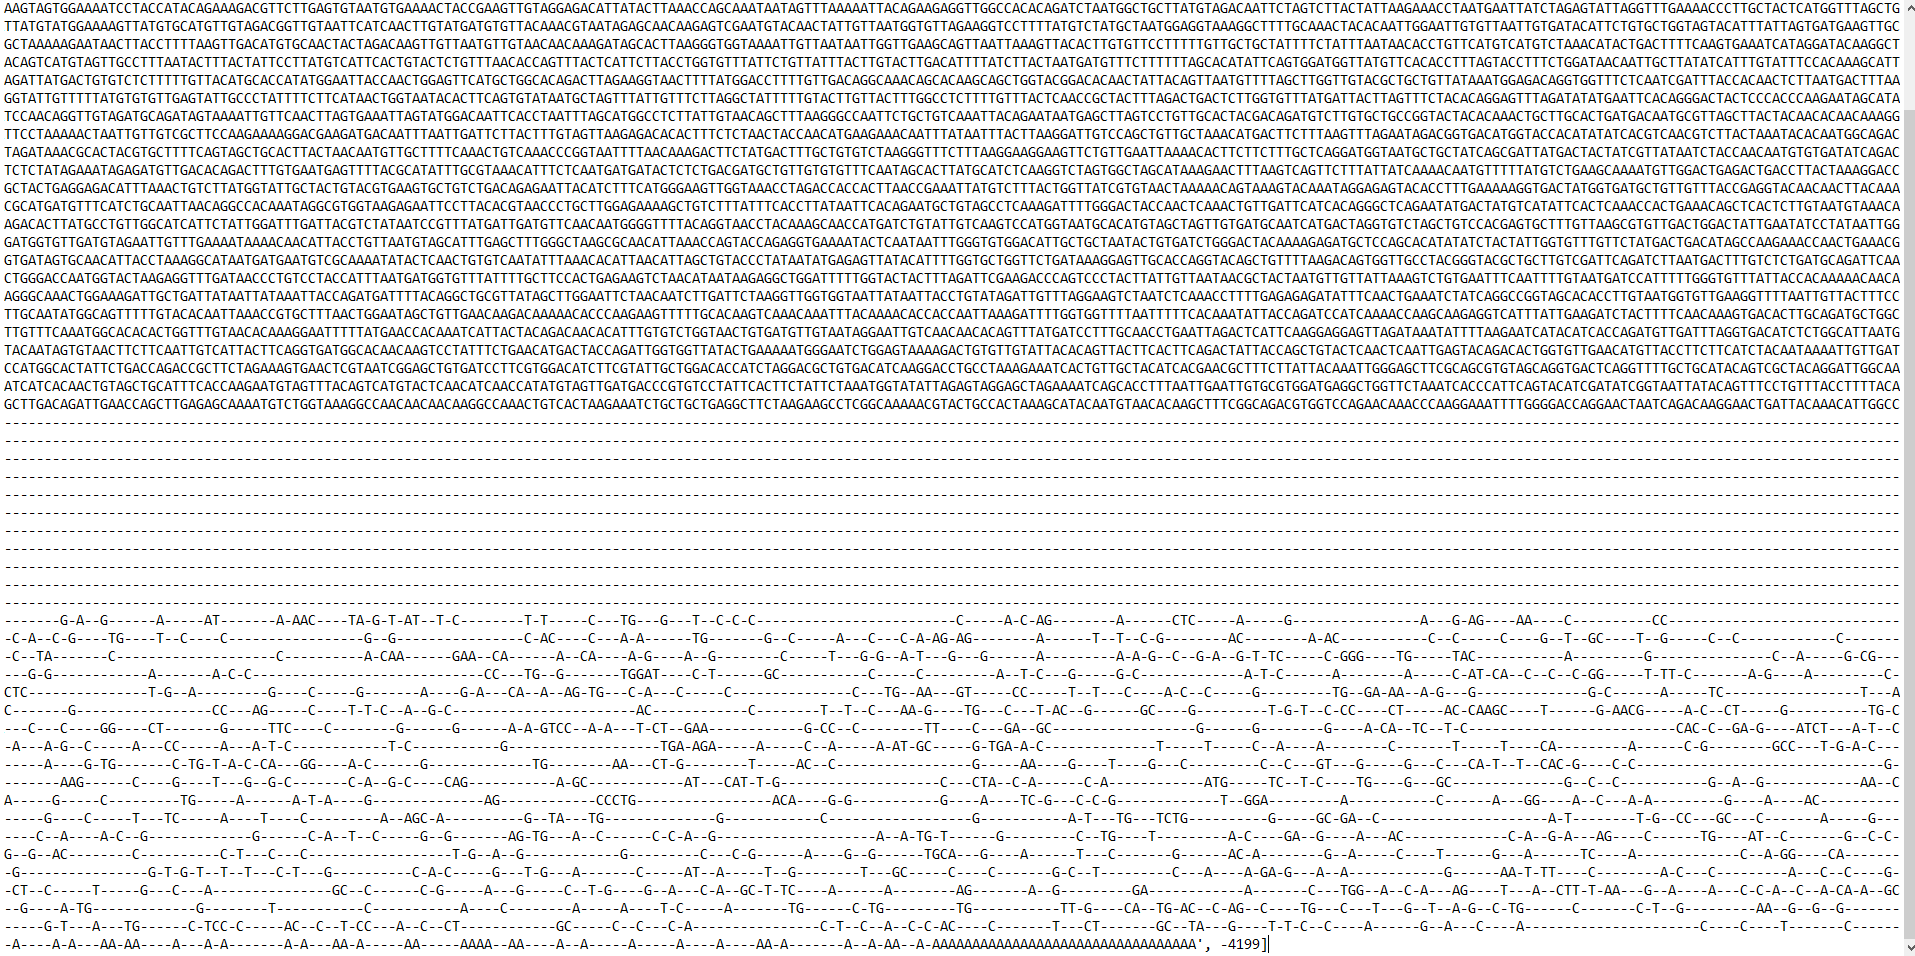
\includegraphics[scale = 0.347]{Images/Needleman/homemade needleman.png}
    \caption{Extrait de l'alignement du génome du SARS-CoV-2 avec l'ARNm du vaccin de Pfizer/BioNTech. (Match = 5, Mismatch = -5, gap = -1)}
    \label{alignement du génome du SARS_CoV-2 avec l'ARNm du vaccin de Pfizer/BioNTech. (Match = 5, Mismatch = -5, gap = -1)}
\end{figure}


D'après cet alignement, la région du génome correspondant à l'ARNm du vaccin se situe entre les nucléotides n°11330 jusqu'à la fin (le génome possède au total 29903 nucléotides). Cependant, on constate un nombre important de gaps séparant les nucléotides du vaccin. Ceci est assez peu précis pour localiser précisément l'emplacement gène "spike" dans le génome du virus.

\newpage
Voici  ci-dessous un autre alignement, mais cette fois-ci en utilisant un aligneur de séquences en ligne~\cite{EMBOSS}:


\begin{figure}[!h]
    \centering
    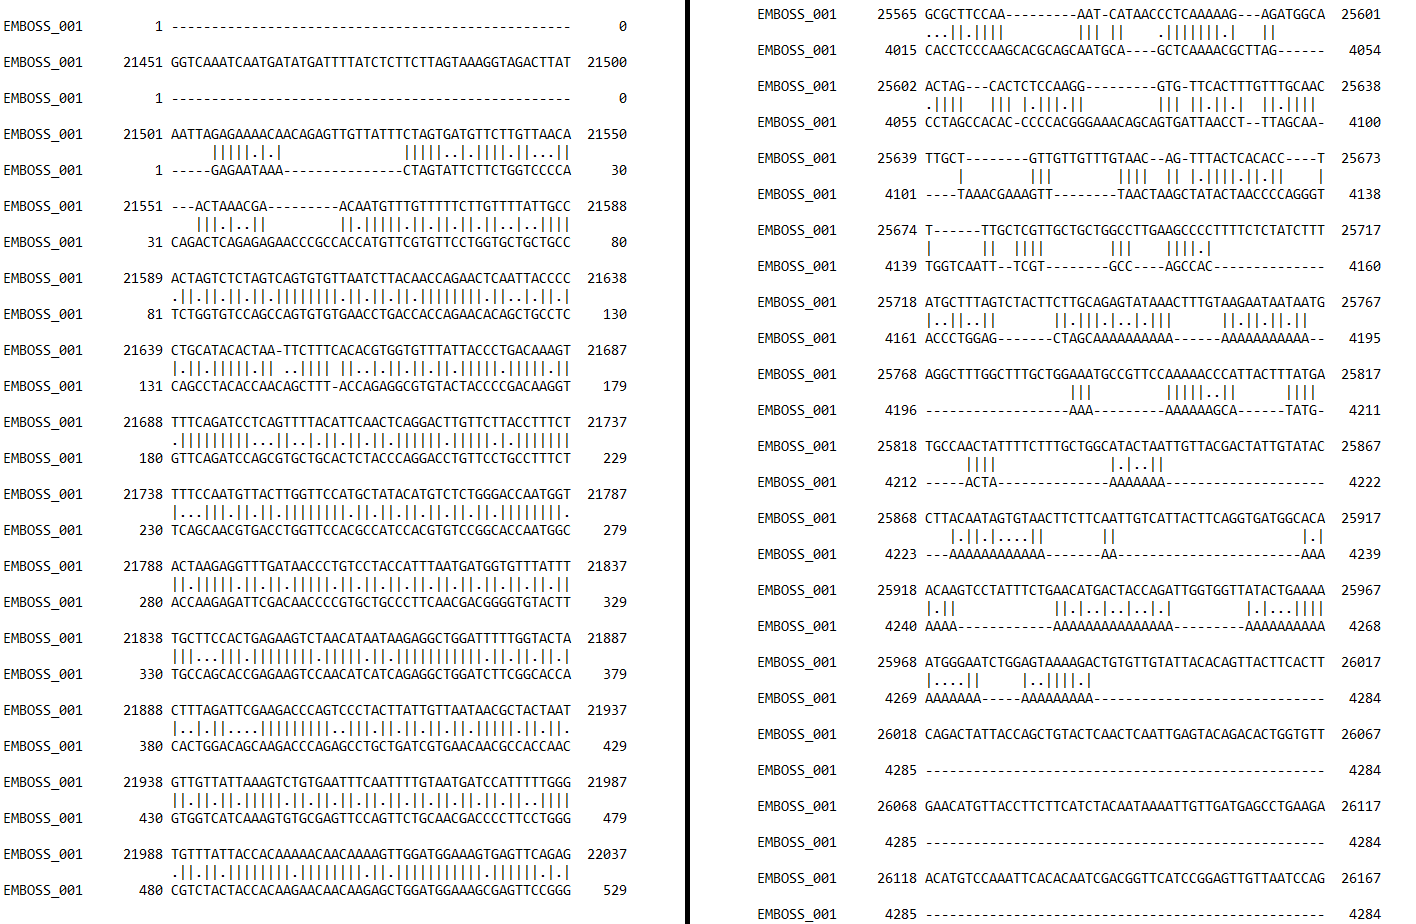
\includegraphics[scale = 0.45]{Images/Needleman/emboss needleman.png}
    \caption{Extraits de l'alignement du génome du SARS-CoV-2 avec l'ARNm du vaccin de Pfizer/BioNTech. (EMBOSS)}
\end{figure}

Ici, on constate tout de suite une quasi absence de gaps entre les nucléotides de la séquence d'ARNm du vaccin. Ceci induit une localisation beaucoup plus exacte du gène "spike" dans le génome du SARS-CoV-2.\\
D'après cet alignement, le gène semble commencer au 21506e nucléotide du génome, et semble se terminer vers le 25739e nucléotide (en ne comptant pas la queue poly-A de la séquence d'ARNm).\\

Voici un document issu du National Center for Biotechnological Information (NCBI) montrant précisément la localisation du gène "spike" pour le SARS-CoV-2 \cite{SPIKE} :

\begin{figure}[!h]
    \centering
    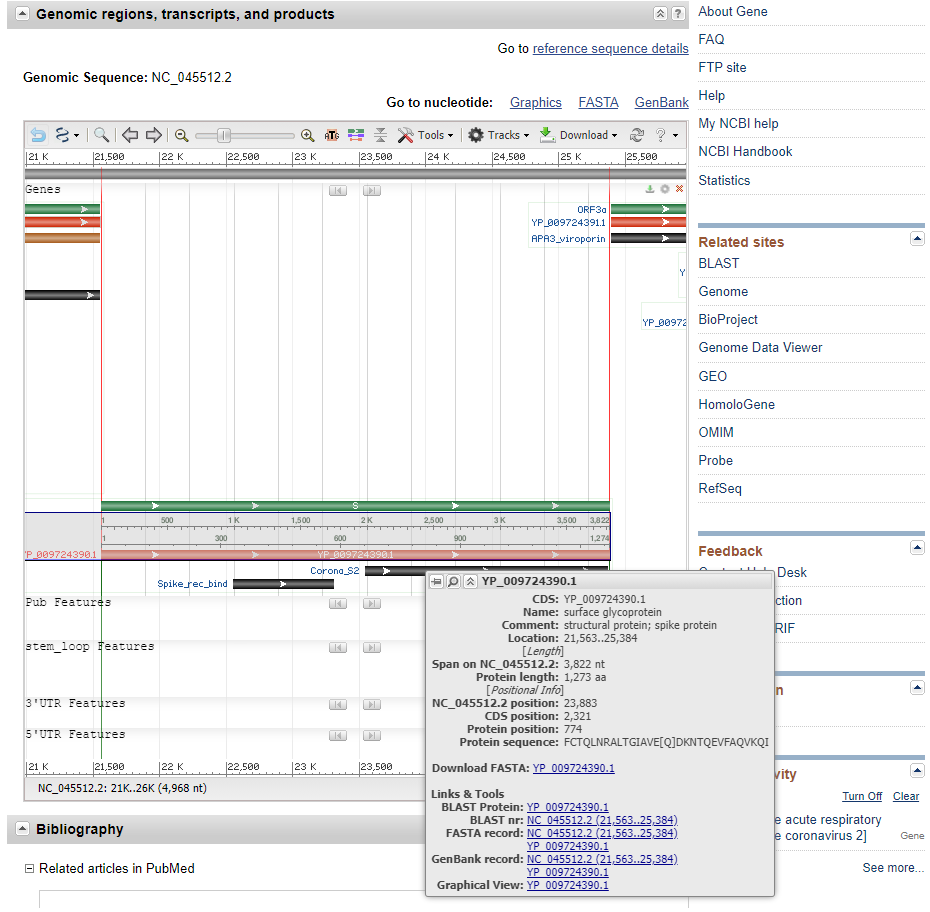
\includegraphics[scale = 0.6]{Images/Needleman/real spike.png}
    \caption{Localisation du gène "spike" dans le génome du coronavirus SARS-CoV-2}
\end{figure}

D'après ce document, le gène se situe entre les nucléotides 21563 à 25384, ce qui est très proche des résultats précédents. Mais alors, comment expliquer cette différence entre notre algorithme et l'algorithme EMBOSS?\\

La différence majeure réside en l'ajout d'un coût d'extension de gap. En effet, l'idée est de mettre un fort coût lors de la création d'un gap, et un très faible coût pour étendre ce gap.

\begin{figure}[!h]
    \centering
    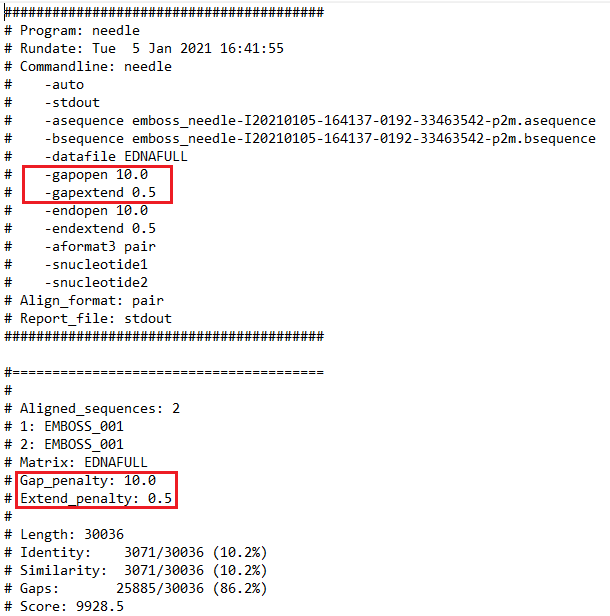
\includegraphics[scale = 0.8]{Images/Needleman/param.png}
    \caption{Paramètres utilisés par l'algorithme de Needleman EMBOSS}
\end{figure}

\newpage

En prenant comme dans l'exemple ci-dessus un coût de création de gap de 10 et un coût d'extension de gap de 0.5, on privilégie l'ajout de peu de gaps de grande taille, plutôt que de nombreux petits gaps. A l'exécution, cela augmente grandement la précision de l'alignement puisque mettre de nombreux petits gaps comme dans nôtre alignement couterait trop cher.\\

Ainsi, implémenter un coût d'extension de gap est une bonne piste d'amélioration pour notre algorithme, et permettrait d'obtenir des résultat beaucoup mieux exploitables pour une utilisation concrète en génomique.

\newpage

\section{Tests et performances}
Dans cette partie, nous présentons les tests et performances de nos fonctions, et nous les comparons à la complexité théorique calculée dans la partie précédente.

\subsection{Fonctions utilitaires}
Pour faciliter la mesure des performances et même le test de différentes fonctions, une poignée de fonctions utilitaires a été programmée. Parmi ces fonctions, il y a:
\begin{itemize}
    \item \texttt{measure\_single\_call}: qui mesure un seul appel à une fonction, avec l'argument \texttt{args} et retourne un tuple qui contient la taille d'argument et le temps d'exécution en seconde.
    \item \texttt{func\_performance}: qui prendra comme arguments une fonction, un tableau d'arguments et l'index ou les indices des arguments dont dépend l'exécution de la fonction. Il y a aussi des arguments moins pertinents comme celui qui permet de demander le trier par temps d'exécution ou par taille d'argument, ou bien un argument en booléen qui indiquent si nous voulons une figure ou non. Et enfin le \texttt{tick\_spacing} qui spécifie l'espacement entre les graduations de l'axe des abscisses. La fonction renvoie une table qui contient un tuple dont la taille de l'argument et le temps d'exécution sont respectivement en seconde.
    \item \texttt{funcs\_performance}: qui est plus ou moins similaire à \texttt{func\_performance} sauf qu'il prend un tableau de fonctions. Le tri basé sur le temps d’exécution n’existe pas ici car il n’a pas de sens, puisque différentes fonctions ont des temps d’exécution différents, les arguments seront donc toujours triés dans l’ordre croissant. Les performances des différentes fonctions seront tracées dans le même graphique avec des couleurs différentes pour permettre une comparaison plus facile entre différentes versions de fonctions. Cette fonction renverra une table contenant la taille de l'argument, la paire de temps d'exécution pour chaque fonction respectivement.
    \item \texttt{plot\_multi\_graph}: Cette fonction a le même objectif que la fonction mentionnée ci-dessus mais au lieu de passer directement les fonctions et de mesurer leur temps d'exécution, elle prend les coordonnées précalculées et les trace. Cette fonction prend également les légendes pour chaque graphique.
    \item \texttt{arg\_generator}: C'est peut-être la fonction la plus importante car elle peut être utilisée pour alimenter les fonctions avec de nombreux arguments générés pseudo-aléatoirement\footnote{En raison de la nature déterministe des ordinateurs, les soi-disant nombres générés aléatoirement ne sont pas vraiment aléatoires. D'où l'appellation pseudo-aléatoire. (Nous utiliserons les deux termes de manière interchangeable dans le rapport, mais ce que nous voulons vraiment dire est pseudo-aléatoire)}. Cette fonction a beaucoup d'arguments et son comportement change légèrement en fonction de la valeur de ses arguments. Les arguments \texttt{start}, \texttt{N} et \texttt{stride} indiquent où la génération d'argument va commencer, où elle va se terminer et les étapes de la même manière qu'une boucle \texttt{for}. Le type indique si nous générons un groupe de chaînes ou un tableau de nombres. Si la fonction génère une chaîne, l'argument \texttt{samples} spécifie quels caractères seront dans la chaîne, si l'argument \texttt{same\_size} est défini sur \texttt{False}, la longueur des chaînes sera choisie au hasard entre \texttt{lower} et \texttt{upper}, sinon la longueur sera itérée de manière croissante. Si la fonction génère des nombres, les nombres \texttt{lower} et \texttt{upper} spécifieront la plage des nombres générés aléatoirement dans le tableau, et le tableau des nombres augmentera linéairement. Enfin, il y a \texttt{variant\_arg\_pos} et \texttt{static\_args}, \texttt{variant\_arg\_pos} spécifiera l'emplacement des différents arguments, tandis que \texttt{static\_arguments} sera la valeur des arguments qui ne change pas ces deux peuvent être utiles pour les fonctions dont la complexité ne dépend que de quelques arguments et pas de tous d'entre eux (comme l'algorithme de Needleman-Wunsch) connaissant ces deux arguments (le dernier peut être \texttt{None}), nous pouvons remplir tous les arguments de la fonction. La fonction renvoie donc à la fin de son execution une liste d'arguments générés pseudo-aléatoirement.
    \item \texttt{func\_performance\_mt}: identique à \texttt{func\_performance} mais utilise plusieurs processus. Elle applique la fonction donnée en paramètre aux arguments du tableau d'entrée, mais de manière simultanée. Elle trace ensuite le résultat sur un graphique.
    \item \texttt{funcs\_performance\_mt}: identique à \texttt{func\_performance} mais utilise plusieurs processus. Elle applique \texttt{func\_performance\_mt} sur toutes les fonctions données en paramètre en parallèle puis trace le résultat.
    \item \texttt{funcs\_performance\_mt\_v2}: identique à \texttt{funcs\_performance\_mt} mais le processus de parallélisation se fait à un niveau plus profond. Il appellera en série \texttt{func\_performance\_mt} pour chaque fonction, parallélisant ainsi l'exécution de la fonction qui nous intéresse sur ses arguments.
\end{itemize}
Vous pouvez peut-être remarquer le suffixe \texttt{mt}, dans les trois dernières fonctions, qui signifie multi-threading. Mais en réalité, ces fonctions utilisent le \textsl{multi-processing} et non le \textsl{multi-threading}. Avec Python, même lors de l'utilisation du \textsl{multi-threading}, il y a de grandes chances que le code soit exécuté de manière séquentielle en raison de l'interférence du GIL\footnote{Le Global Interpreter Lock est un verrou (lock) que l’interpréteur utilise afin d’être thread-safe sur le comptage des références du ramasse-miette.} avec l'exécution des \textsl{threads}. Au lieu de cela et pour surmonter tout le problème, plusieurs processeurs sont utilisés en utilisant le paquet \texttt{multiprocesseur} de python.\\
La raison derrière l'implémentation de telles fonctions en exécutions simultanées est que l'exécution séquentielle des tests de performance pourrait potentiellement prendre beaucoup de temps, en particulier avec des fonctions de complexité exponentielle comme \texttt{lev} et \texttt{needleman\_all}. Et comme il n'y a pas de dépendances lors de l'exécution de ces fonctions\footnote{Et du coup l'absence de nécessité d'utiliser un mécanisme de verrouillage \textsl{Locking Mechanism}} sur différents arguments, il y a donc une opportunité pour paralléliser l'exécution de l'ensemble des fonctions de test de performance et profiter du package \texttt{multiprocessing} que Python fourni par défault. \\
Nous avons aussi remarqué que \texttt{arg\_generator}, qui était principalement utilisé et implémenté pour les tests de performances, peut être légèrement modifié et utilisé pour réaliser des tests générés pseudo-aléatoirement. Donc, un tas de ces tests ont été mis en œuvre partout où nous le pouvions dans nos fichiers de tests.



\subsection{Les tests des fonctions}
Tous les tests ont été écrits en utilisant \texttt{pytest} et en s'appuyant sur les principes \textit{Right-BICEP}. 
Les librairies \texttt{BioPython} et \texttt{NumPy} ont été utilisées aussi en testant avec ses fonctions prédéfinies. Toutefois, pour des tests plus simples et objectifs, des tests aléatoires ont été réalisés pour certaines fonctions avec la fonction \texttt{arg\_generator} défini dans le fichier \texttt{src/performance.py}.



\subsubsection{Les fonctions de statistiques}
Les tests de toutes les fonctions calculant les statisques ont été faits en parcourant toutes les situations possibles (dans le cadre du projet); des cas de listes vides ont été ajoutés, les fonctions renvoient \texttt{None}. De plus des tests avec la fonction \texttt{arg\_generator} ont été faits, pour choisir des nombres pseudo-aléatoires. Par ailleurs, lors du test de \texttt{quartile} avec le module \texttt{NumPy}, le choix de l'interpolation était nécessaire. Au début, elle n'était pas précisée, donc par défaut l'interpolation était linéaire, or celle de la fonction \texttt{quartile} ne l'est pas donc, il y a eu des échecs, puis après modification de l'interpolation\footnote{en \texttt{lower} et \texttt{higher}} les tests sont passés avec succès.



\subsubsection{Les fonctions codons}
Des différents tests ont été écrits pour les trois versions de \texttt{codons}. 
Pour la fonction \texttt{codons}, des tests codés en dur ont été réalisés, ainsi que deux autres fonctions \texttt{test\_codons\_bio\_seq} et \texttt{test\_codons\_gen}. En effet, \texttt{test\_codons\_bio\_seq} teste la fonction \texttt{codons} en utilisant le module \texttt{Seq}  prédéfini de la librairie \texttt{biopython}. Toutefois, à travers la fonction, on a adapté les résultats de \texttt{Seq} de sorte à ce que ce soit compatible aux résultats de la fonction \texttt{codons} qui est conforme à la documentation comme expliqué dans la partie \ref{subsec:imp_codons}.
Quant à \texttt{test\_codons\_gen}, elle est conforme à \texttt{test\_codons\_bio\_seq} mais en génèrant pseudo-aléatoirement les arguments pour les tests.
C'est le cas aussi pour \texttt{test\_codonsv2\_gen} et \texttt{test\_codonsv3\_gen} qui sont conformes respectivement à \texttt{test\_codon\_v2} et \texttt{test\_codons\_v3\_bio\_seq}.
Il faut noter aussi qu'à travers les tests on a constaté que la fonction \texttt{codon\_v2} est la version la plus conforme à la fonction \texttt{translate()} du module \texttt{Seq} de \texttt{biopython}.



\subsubsection{Les fonctions : distance de Levenshtein}
Comme dans l'implémentation de l'algorithme de Levenshtein trois versions ont été réalisées, toutes les versions ont été alors testées.
Deux méthodes de tests ont été proposées. La première consiste à créer un tableau (liste des listes) où on entre manuellement des arguments à tester sous la forme de : [chaine1\footnote{La première séquence pour le calcul de la distance de Levenshtein}, chaine2\footnote{La deuxième séquence pour le calcul de la distance de Levenshtein}, entier\footnote{La distance de Levenshtein entre les deux séquences (le résultat attendu) }]. Ensuite, on effectue les tests par les fonctions \texttt{test\_rec} et \texttt{test\_dp} en testant respectivement \texttt{lev\_rec} et \texttt{lev\_dp}. Quant à la fontion \texttt{test\_lev\_total}, elle teste tous les fonctions à savoir \texttt{lev\_rec}, \texttt{lev\_dp} et \texttt{lev} en les comparant entre elles.
Enfin, la deuxième méthode de test, décrite par la fonction \texttt{test\_gen\_lev}, consiste à générer les arguments aléatoirement\footnote{par la fonction \texttt{arg\_generator}} tout en comparant les trois versions entre elles. 



\subsubsection{Les fonctions : algorithme de Needleman-Wunsch}
Le test des fonctions de Needleman n'était pas aussi simple que d'autres fonctions. De nombreux problèmes ont été rencontrés lors de la mise en œuvre. Tout d'abord, nous voulions comparer les résultats de nos fonctions à ceux de \texttt{BioPython}. Nous avons commencé par utiliser le module \texttt{BioPython} \texttt{pairwise2.align}, ce qui nous a posé problème car la fonction ne renvoie pas tous les alignements possibles. Au début, nous pensions que c'était un bug et nous l'avons signalé sur la page BioPython sur GitHub\footnote{\url{https://github.com/biopython/biopython/issues/3453}}. Un contributeur appelé \href{https://github.com/mdehoon}{\textsl{mdehoon}} nous a suggéré d'utiliser le module le plus récent \texttt{PairwiseAligner} de \texttt{BioPython}, nous l'avons donc choisi pour nos tests. Un autre contributeur appelé \href{https://github.com/MarkusPiotrowski}{Markus Piotrowski} a expliqué que le module \texttt{pairwise2.align} n'est pas défectueux mais il ne renvoie pas tous les alignements possibles car certains d'entre eux sont redondants et n'ont pas d'utilisation significative dans la vie réelle; et car la sortie d'alignement est limitée à 1~000 pour les fonctions de \texttt{pairwise2.align}. Les tests dans l'ensemble nous ont permis de découvrir quelques bugs qui ont été corrigés par la suite. Certains de ces bugs étaient mineurs, comme les bugs qui viennent d ufait que python effectue une copie superficielle au lieu d'une copie profonde par défault pour les tableaux. D'autres étaient plus fondamentaux et liés à la logique de l'algorithme lui-même.\\
Pour tester toutes les fonctions de Needleman-Wunsch avec leurs différentes versions, nous avons utilisé quelques tests écrits à la main avec un tas de différents tests générés pseudo-aléatoirement. 
La quantité de tests générés peut être contrôlée avec les paramètres déclarées en haut des fichiers de test\footnote{les autres fichiers de test contenant des tests générés de manière pseudo-aléatoire suivent la même tendance}. Ces paramètres sont utiles pour effectuer plus de tests, les réduire ou les désactiver complètement, ce qui devient rapidement pratique, d'autant plus que certaines fonctions prennent beaucoup de temps à s'exécuter.



\subsection{Les tests de performance}



\subsubsection{Les fonctions de statistiques}
Les tests de performances sont réalisés sur des listes d'éléments générés pseudo-aléatoirement\footnote{avec la fonction \texttt{arg\_generator}}, elles sont de taille entre 1 à 100~000.
\paragraph{\texttt{moyenne}} a une complexité théorique linéaire $\Theta(n)$ pour la fonction \texttt{moyenne}. Selon le test de performances, voir figure~\ref{perfmoy}, l'allure de la courbe du temps d'exécution de \texttt{moyenne} semble plutôt linéaire, comme le prévois la complexité théorique.
     \begin{figure}[!h]
        \centering
        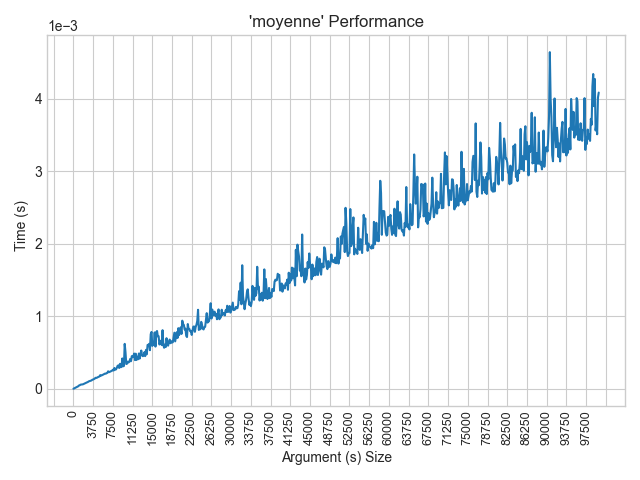
\includegraphics[scale=0.75]{Images/Performance/Stats/performance_moyenne_100000.png}
        \caption{Test de performance de la fonction \texttt{moyenne} sur des listes de taille 1 à 100~000}
        \label{perfmoy}
    \end{figure}
\paragraph{\texttt{proportion}} a une complexité théorique linéaire $\Theta(n)$. D'après le test de performance, voir figure~\ref{perfprop}, le temps de réponse de \texttt{proportions} semble assez linéaire, comme l'indique la complexité théorique.
     \begin{figure}[!h]
        \centering
        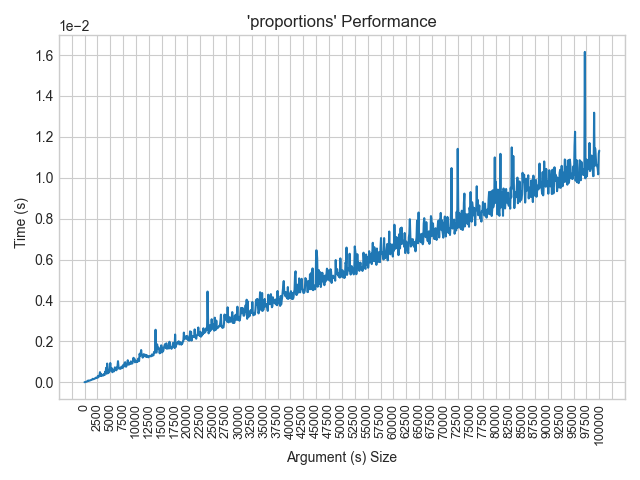
\includegraphics[scale=0.8]{Images/Performance/Stats/performance_proportions_100000.png}
        \caption{Test de performance de la fonction \texttt{proportions} sur des listes de taille 1 à 100~000}
        \label{perfprop}
    \end{figure}
\paragraph{\texttt{mediane}} a une complexité théorique quasi-linéaire $\Theta(nlog(n))$ dans le pire des cas, et linéaire ($\Theta(n)$) dans le meilleur des cas. Selon le test sur la figure~\ref{perfmed}, le temps de réponse de \texttt{mediane} semble quasi-linéaire (linéaire légèrement arondi), cela ressemble à la complexité théorique.
     \begin{figure}[!h]
        \centering
        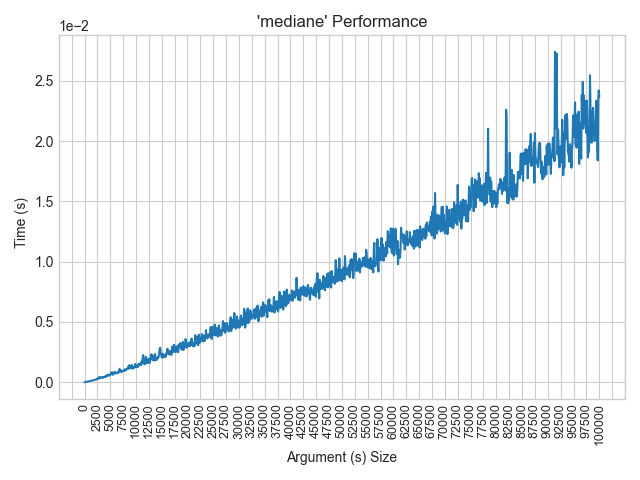
\includegraphics[scale=0.8]{Images/Performance/Stats/performance_mediane_100000.png}
        \caption{Test de performance de la fonction \texttt{mediane} sur des listes de taille 1 à 100~000}
        \label{perfmed}
    \end{figure}
\paragraph{\texttt{quartile}} a la même complexité que la fonction \texttt{mediane} $\Theta(nlog(n))$ dans le pire des cas, et linéaire $\Theta(n)$ dans le meilleur des cas). D'après les tests de performance sur la figure~\ref{perfquart}, le temps de réponse de \texttt{quartile} semble quasi-linéaire (linéaire légèrement arondi), ce qui est comparable à la complexité théorique.
     \begin{figure}[!h]
        \centering
        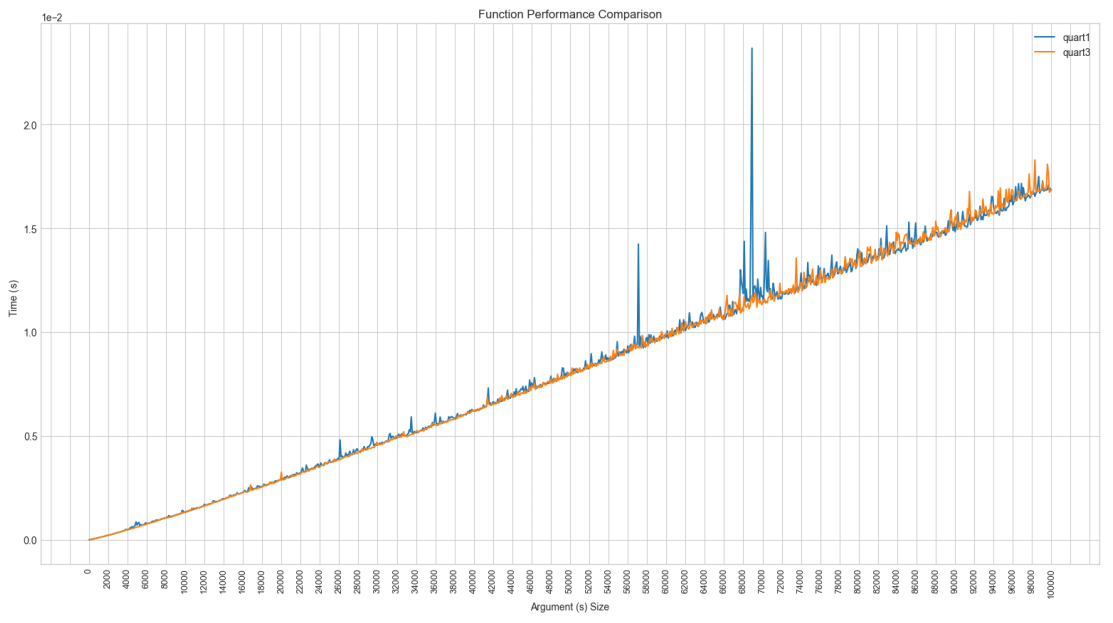
\includegraphics[scale=0.6]{Images/Performance/Stats/performance_quartile_100000.png}
        \caption{Test de performance de la fonction \texttt{quartile} sur des listes de taille 1 à 100~000}
        \label{perfquart}
    \end{figure}
\paragraph{\texttt{variance}} a une complexité théorique linéaire $\Theta(n)$. Selon le test de performance, voir figure~\ref{perfvar}, le temps de réponse de \texttt{variance} est linéaire, comme le prévoit la complexité théorique.
     \begin{figure}[!h]
        \centering
        \includegraphics[scale=0.8]{Images/Performance/Stats/performance_variance_100000.png}
        \caption{Test de performance de la fonction \texttt{variance} sur des listes de taille 1 à 100000}
        \label{perfvar}
    \end{figure}
\paragraph{\texttt{ecart\_type}} se comporte comme la fonction \texttt{variance}, elle a une complexité théorique linéaire $\Theta(n)$. Selon les tests de performances, voir figure~\ref{perfecartt}, le temps de réponse de \texttt{ecart\_type} est linéaire, comme la complexité théorique de la \texttt{variance}.
     \begin{figure}[!h]
        \centering
        \includegraphics[scale=0.8]{Images/Performance/Stats/performance_ecart_type_100000.png}
        \caption{Test de performance de la fonction \texttt{ecart\_type} sur des listes de taille 1 à 100~000}
        \label{perfecartt}
    \end{figure}
\paragraph{\texttt{intervalle\_interquartile}} appelle deux fois la fonction \texttt{quartile} pour une soustraction des deux, elle a une complexité théorique quasi-linéaire en $\Theta(nlog(n))$. D'après nos tests de performances, voir figure~\ref{perfintquart}, l'allure de la courbe du temps d'exécution est quasi-liénaire.
     \begin{figure}[!h]
        \centering
        \includegraphics[scale=0.78]{Images/Performance/Stats/performance_interquartile_100000.png}
        \caption{Test de performance de la fonction \texttt{intervalle\_interquartile} sur des listes de taille 1 à 100~000}
        \label{perfintquart}
    \end{figure}

\newpage

\subsubsection{Les fonctions codons}
Les tests de performances des fonctions \texttt{codons} sont réalisés sur des chaînes de caratères générées aléatoirement, elles sont de taille entre 1 et 9~000.
Les trois fonctions \texttt{codons}, \texttt{codon\_v2} et \texttt{codon\_v3} ont une complexité théorique linéaire $\Theta(n)$. Selon le test de performances, voir figure~\ref{perfcodons}, l'allure des courbes du temps d'exécution des fonctions semblent plutôt linéaire, ce qui est conforme à la complexité théorique.

     \begin{figure}[!h]
        \centering
        \includegraphics[scale=0.8]{Images/Performance/Codons/performance_codons_comp3.png}
        \caption{Test de performance des fonctions \texttt{codons}, \texttt{codons\_v2} et \texttt{codons\_v3}}
        \label{perfcodons}
    \end{figure}



\subsubsection{Les fonctions : distance de Levenshtein}
Nous avons discuté dans la section~\ref{subsec:lev} que la complexité théorique de l'algorithme de Levenshtein est $O(n.m)$ pour \texttt{lev\_dp} et \texttt{lev} et $O(3^{n+m})$ pour \texttt{lev\_rec} où n, m sont respectivement la longueur de la première et la deuxième séquence. Nous allons vérifier ces résultats théoriques et comparer les différentes versions de l'implémentation Levenshtein. Il est important de noter que pour faciliter la mesure, le tracé des graphiques, et pour avoir des résultats cohérents, nous avons exécuté nos tests de performances sur des arguments de même taille à chaque fois. En utilisant cette simplification les complexités en $O(n.m)$ deviendront des complexités en $O(n^{2})$. Puisque nous savons déjà de quoi dépend la complexité de l'algorithme, cette simplification n'aura pas d'impact sur les résultats ni sur la vérification de la complexité hypothétique.

\paragraph{\texttt{lev}}
Il s'agit de la version itérative de l'implémentation de l'algorithme de Levenshtein utilisant la programmation dynamique. Nous voyons, en effet, que cette version est la plus rapide parmi toutes les autres implémentations. 
On remarque également la même forme de courbure que \texttt{lev\_dp} mais avec des coefficients différents, ce qui vérifie notre hypothèse\footnote{qui dit que les deux ont la même complexité de $O(n.m)$}. La forme d'une courbe ressemble à une fonction $n$ au carré, ceci est compatible avec nos attentes, voir figure~\ref{perflev}.

\paragraph{\texttt{lev\_dp}}
Il s'agit de la version récursive de l'algorithme de Levenshtein utilisant la programmation dynamique. On voit que cette version est plus rapide que \texttt{lev\_rec} (qui est entièrement récursive sans programmation dynamique) mais toujours plus lente que la version itérative, car il y a un surcoût dû à la création de l'environnement de la fonction à chaque appel récursif, voir figure~\ref{perflev}.

    \begin{figure}[!h]
        \centering
        \includegraphics[scale=0.4]{Images/Performance/Levenshtein/performance_levenshtein&dp.png}
        \caption{Test de performance des fonctions \texttt{lev} et \texttt{lev\_dp}}
        \label{perflev}
    \end{figure}

\paragraph{\texttt{lev\_rec}}
Est la fonction la plus lente de toutes et aussi la fonction qui a le plus grand taux de croissance, qui est en fait une croissance exponentielle, voir figure~\ref{perflevrec}. Puisqu'il n'utilise aucune technique de mémorisation et recalcule même les résultats déjà calculés. Ce qui explique sa complexité exponentielle.
\\\\
On peut conclure que l'utilisation de la programmation dynamique optimisera grandement l'implémentation récursive naïve qui permet de réduire sa complexité de $O(3^{n + m})$ à $O(n.m)$.
    
    \begin{figure}[!h]
        \centering
        \includegraphics[scale=0.4]{Images/Performance/Levenshtein/performance_levenshtein_rec.png}
        \caption{Test de performance des fonctions \texttt{lev}, \texttt{lev\_dp} et \texttt{lev\_rec}}
        \label{perflevrec}
    \end{figure}

\newpage

\subsubsection{Les fonctions : algorithme de Needleman-Wunsch}
Nous avons discuté dans la section \ref{subsec:nw_impl} que la complexité théorique de \texttt{needleman} qui produit un seul alignement est $\Theta(n.m)$ et \texttt{needleman\_all} a une complexité de $O(e^{n+m})$ où \textsl{n},\textsl{m} est respectivement la longueur de la première et de la deuxième séquence. 
Nous confirmerons non seulement ces affirmations, mais nous les comparerons également au résultats de performance du module \texttt{PairwiseAligner} de BioPython.
\paragraph{\texttt{needleman}}
La forme du temps d'exécution de \texttt{needleman} ressemble à la courbure d'une fonction $n$ au carré, voir figure~\ref{perfnwnormal}. 

\newpage

    \begin{figure}[!h]
        \centering
        \includegraphics[scale=0.55]{Images/Performance/Needleman-Wunsch/performance_needleman_normal.png}
        \caption{Test de performance des fonctions \texttt{needleman}}
        \label{perfnwnormal}
    \end{figure}
Ce qui est normal puisque nous avons suivi la même stratégie utilisée pour mesurer les performances de Levenshtein, en prenant des arguments de même taille pour simplifier les mesures et le tracé des graphes. On peut donc en conclure que la complexité théorique que nous avons calculée est correcte ($O(n.m)$).
\paragraph{\texttt{needleman\_all} et \texttt{PairwiseAligner}}
En regardant sur le graphique~\ref{perfnwpire} pour le pire des cas, nous remarquons que \texttt{needleman\_all} et \texttt{PairwiseAligner} croissent de façon exponentielle. Les tests de performance ont été réalisés sur des échantillons aléatoires de nucléotides allant de 1 à 7, avec un coût nul pour toutes sortes d'opérations (c'est-à-dire le \textsl{match}, \textsl{mismatch} et le \textsl{gap}). nous pouvons conclure que la borne supérieure que nous avons théoriquement calculée était en fait exacte.\\
À partir du graphique~\ref{perfnwavg} du temps d'exécution en moyen des cas, nous voyons que la courbe de \texttt{needleman\_all} ressemble à un $n^2$ qui est cohérent avec sa complexité moyenne. Cependant, nous remarquons également beaucoup de fluctuations, principalement des sauts vers des valeurs très élevées. Ces sauts peuvent être expliqués par la complexité dans le pire des cas qui est de l'ordre de $O(e^{n+m})$. Ces tests utilisent des matrices de similarité et il n'y a rien de spécial à cela, nous pouvons plutôt choisir la méthode standard et nous obtiendrons des résultats similaires. Nous avons cependant choisi cette version pour varier.\\
    \begin{figure}[!h]
        \centering
        \includegraphics[scale=0.4]{Images/Performance/Needleman-Wunsch/performance_needleman_pire_cas.png}
        \caption{Test de performance des fonctions \texttt{needleman}, \texttt{needleman\_all} et \texttt{nw\_bio\_generic} (cette dernière est la fonction de \texttt{biopython})}
        \label{perfnwpire}
    \end{figure}
    \begin{figure}[!h]
        \centering
        \includegraphics[scale=0.4]{Images/Performance/Needleman-Wunsch/performance_needleman_all_average.png}
        \caption{Test de performance des fonctions \texttt{needleman}, \texttt{needleman\_all} et \texttt{nw\_bio\_generic} (cette dernière est la fonction de \texttt{biopython}) cas moyen}
        \label{perfnwavg}
    \end{figure}
   

Dans l'ensemble, il y a encore une marge d'amélioration pour la fonction \texttt{needleman\_all}. Tout d'abord, nous pouvons éliminer tous les alignements redondants. Deuxièmement, nous pouvons exécuter en parallèle l'étape de retraçage qui est l'étape la plus lourde, avec la plus grande complexité (autrement dit le \textsl{bottleneck}\footnote{le goulot d'étranglement}). Troisièmement, nous pouvons coder la fonction entière dans un langage de programmation de bas niveau comme \textsf{C} ou \textsf{C++} qui s'exécute beaucoup plus rapidement que \textsf{Python}, puis fournir une interface pour pouvoir l'appeler via \textsf{Python} (c'est ce que \texttt{BioPython} fait pour la plupart de ses fonctions).

\newpage

\section{Gestion de projet}
Cette partie est consacrée à la présentation de notre gestion de projet. L'équipe s'est inspiré du cadre méthodologique SCRUM, pour l'organisation de l'équipe et du projet, voir la table~\ref{tab:roles}, la méthode SMART a été utilisé pour le découpage des tâches, voir la table~\ref{tab:SMART}; avant le début du projet une analyse des risques en utilisant la matrice SWOT a été effectuée, voir la figure~\ref{fig:Matrice SWOT}.



\subsection{Équipe de projet}
Ce projet a été réalisé par le groupe 13 dont les membres sont~:
\begin{itemize}
    \item Mohamed Omar CHIDA, le leader développeur du SCRUM, il s'assure le découpage des tâches, s'occupe de régler tous les soucis informatique au sein du projet, et il se charge de trancher lors des débats;
    \item Mathis DUMAS, le développeur côté documentaire, il s'occupe l'exactitude des notions abordées, vérifie les sources de celles-ci et s'occupe des graphes d'analyse du rapport;
    \item Chaima TOUNSI OMEZZINE, le développeur code reviewer, elle s'assure de l'utilité de chaque fonction, la correspondance avec le sujet du projet (le cahier de charges), et vérfie les tests de celles-ci;
    \item Céline ZHANG, le développeur organisateur, elle s'occupe de l'organisation des réunions, du déroulement des réunions, de la répartition des tâches à la fin de celles-ci, de l'avancée du rapport, et elle se charge de rédiger les comptes rendus de réunions.
\end{itemize}
Chaque membre est développeur, donc participe à la conception et à l'écriture des codes.%, en plus des rôles complémentaires spécifiques.
\begin{table}[!h]
\begin{center}
    \begin{tabular}{|l|l|}
    \hline
        Membre de l'équipe 13 & Rôles ou charges \\
    \hline
    \hline
        Mohamed-Omar CHIDA & Leader \\
    \hline
        Mathis DUMAS & Documentation \\
    \hline
        Chaima TOUNSI OMEZZINE & Reviewer \\
    \hline
        Céline ZHANG & Organisateur \\
    \hline
    \end{tabular}
\end{center}
\caption{La répartition des rôles}
\label{tab:roles}
\end{table}

\subsection{Analyse du projet}

\subsubsection{Définition des objectifs}
Les objectifs ont été définis en se basant sur la méthode SMART comme indiqué sur la table~\ref{tab:SMART}: 
\begin{table} [!h]
 \begin{center}
 \begin{tabular}{|c||l|l|}
 \hline
  & Critère & Indicateur \\
 \hline
 S & Spécifique & Objectif clair, précis et sans ambiguité \\
 \hline
 M & Mesurable & Objectif quantifié permettant de mesurer l'état d'avancement \\
 \hline
 A & Ambitieux et Atteignable & Objectif représentant un défi atteignable et non démotivant \\
 \hline
 R & Réaliste & Objectif envisageable et suffisamment motivant \\
 \hline
 T & Temporellement défini & Objectif défini et délimité dans le temps \\
 \hline
 \end{tabular}
 \end{center}
 \caption{La méthode SMART}
 \label{tab:SMART}
 \end{table}


\subsubsection{Analyse des risques: Matrice SWOT}
Nous avons évalué les risques du projet en utilisant la matrice SWOT sur la figure \ref{fig:Matrice SWOT}.
        \begin{figure}[!h]
             \centering
             \includegraphics[scale = 0.5]{Images/Gestion de Projet/Matrice_swot.png}
             \caption{La matrice SWOT du projet}
             \label{fig:Matrice SWOT}
        \end{figure}

\subsection{Organisation du projet}
\subsubsection{Durée}
Le projet a commencé 18 Octobre 2020 et s'est terminé le 5 Janvier 2020, pour une durée de 80 jours. Cette version du rapport a été terminée le 5 Janvier 2021.

\subsubsection{Le cadre méthodologique SCRUM}
% SCRUM est un cadre méthodologique et non pas une méthode.

Pour une meilleure organisation, nous avons choisi d'adapter une gestion de projet agile avec SCRUM. On a estimé que l'adaptation collective et rapide sera plus productive et plus constructive pour tous les membres de l'équipe.

Par conséquent, nous nous sommes basés sur les 3 piliers fondamentaux de SCRUM: 
\begin{itemize}
    \item Transparence (visibilité concrète sur la situation)
    \item Inspection (détection des écarts par rapport aux objectifs)
    \item Adaptation (réctification de ces écarts par rapport aux objectifs)
\end{itemize}

Conformément à ce cadre, un ordonnancement du product backlog a été effectué, au début. Nous avons divisé les tâches sur des \textsl{sprints} fixés afin de pouvoir concevoir, réaliser et tester les nouvelles fonctionnalités au fur et à mesure.
En effet, pour chaque \textsl{sprint} on fixe un objectif à court terme et on se lance dans la réalisation. Une fois cet objectif atteint, nous discutons et nous nous adaptons à la situation, à travers les réunions hebdomadaires. \\
Toutes ces organisations ont été mis en oeuvre dans le tableau Trello\footnote{\url{https://trello.com/b/N92bj53G/projet-grp13}} comme illustré dans la figure~\ref{fig:Trellomid}.
    \begin{figure}[!h]
        \centering
        \includegraphics[scale = 0.5]{Images/Gestion de Projet/Trello/trello_milieu.PNG}
        \caption{L'organisation du projet sur Trello}
        \label{fig:Trellomid}
    \end{figure}

L'organisation du tableau Trello était comme suit:
\begin{itemize}
    \item \textbf{Resources :} c'est les documations qu'il faut faire.
    \item \textbf{Backlog :} la liste de tâches priorisées.
    \item \textbf{Current Sprint :} le Sprint au cours de réalisation.
    \item \textbf{In Progress :} les tâches en cours de réalisation.
    \item \textbf{Production :} les tâches finies.
\end{itemize}
Pour chaque tâche il y a un ensemble d'étiquettes par lesquelles on pourrait avoir une idée sur la tâche et son avancement.
On distingue principalement des étiquettes qui précisent la nature de la tâches comme~:
\begin{itemize}
    \item \textbf{Algorithmic :} si la tâche consiste à écrire un algorithme ou implémenter une fonction. Par exemple, l'algorithme de Needleman ou la distance de Levenshtein.
    \item \textbf{Statistical Analysis :} est attribuée pour toutes les tâches en relation avec l'analyse descriptive.
    \item \textbf{Utility :} est attribuée aux tâches qui consistent à implémenter des fonctions utiles pour les fonctions de base. Par exemples, la fonction \texttt{fasta\_to\_genome}.
    \item \textbf{Benchmark :} est attribuée aux tâches de performances.
    \item \textbf{Report :} si la tâche est en relation avec la rédaction du rapport.
    \item \textbf{Presentation :} si la tâche est en relation avec la réalisation de la présentation.
\end{itemize}
Des autres étiquettes qui permettent de suivre l'avancement des tâches:
\begin{enumerate}
    \item \textbf{Research :} la phase de documentation 
    \item \textbf{Design/Conception :} la phase de la conception de l'algorithme.
    \item \textbf{Implémentation :} la phase de l'implémentation de l'algorithme.
    \item \textbf{Code Review :} une étiquette qui est attribuée à la tâche après l'implémentation pour que les autres développeurs passent vérifier le code.
    \item \textbf{Testing :} la phase des tests.
    \item \textbf{Bug Proof :} quand une tâche est finie, on attribue cette étiquette et on la glisse dans la colonne Production.
\end{enumerate}
Finalement, il y a aussi des étiquettes qui précisent le caractère de la tâche~:
\begin{itemize}
    \item \textbf{Basic :} des tâches basiques qui sont prioritaire.
    \item \textbf{Flex :} des tâches supplémentaires non demandées par l'énoncé.
    \item \textbf{Issue :} est attribuée à la tâche si le développeur chrgé par celle-ci a des problèmes.
\end{itemize}



\subsection{Outils de travail}



\subsubsection{Communication}
Les principales outils de communication sont~: \textsf{Discord}, \textsf{Messenger}, \textsf{GitHub}
\paragraph{\textsf{Discord}} a été utilisé pour communiquer en messages, pour organiser des réunions, montrer les codes, streamer des explications, et éventuellement envoyer des documents.
\paragraph{\textsf{Messenger}} est principalement utilisé pour la communication des réunions, l'échange des disponibilités et la discussion des particularités des tâches lors des \textsl{sprint} en dehors des réunions.
\paragraph{\textsf{GitHub}} a permis de communiquer avec les contributeurs de la bibliothèque \texttt{biopython} afin de pouvoir comprendre l'utilisation des modules (\texttt{Aligner}, \texttt{pairwise2}).



\subsubsection{IDE}
Selon les préférences de chaque membre, plusieurs outils de programmation ont été utilisés, les IDE~: \textsf{PyCharm}, \textsf{Visual Studio Code} et \textsf{IDLE}.



\subsubsection{Partage du travail}
Tout au long du projet, nous avons utilisé le dépot \textsf{GitLab} fournit par l'école, \textsf{Google Drive} (pour les débuts), et \textsf{workupload}\footnote{\url{https://workupload.com/}} pour le partage de gros documents (comme les échantillons de séquences du génome). Nous avons crée plusieurs répértoires pour organiser nos fichiers: 
\begin{itemize}
    \item \texttt{src} pour les fichiers de code.
    \item \texttt{tests} pour les fichiers test.
    \item \texttt{app} pour les applications des algorithmes.
    \item \texttt{rapport} pour enregistrer les résultats des applications.
    \item \texttt{genome} où on ajoute les fichiers .fasta pour les applications.
\end{itemize}

\subsubsection{Rédaction du rapport}
Le rapport a été rédigé sur \textsf{Overleaf} permettant aux membres de modifier leurs parties simultanément, cela facilite la compilation du rapport (évitant les soucis de packages ou versions). \ 
Un répertoire \texttt{rapport} a été mis en place aussi sur le dépot \textsf{Gitlab} dans lequel est rassemblé l'ensemble des résultats des applications.



\subsection{Les réunions de projet}
Les réunions ont été essentielles pour planifier les \textsl{sprints}, régler les problèmes rencontrés. Nous avons eu 12 réunions de groupe sur \textsf{Discord} (de durée totale de 39 heures) qui sont listées dans le tableau~\ref{tab:reunions}, pour lesquelles des comptes rendus de réunion ont été écrites, ils se trouvent dans les annexes. Par ailleurs quelques \textsl{stand-up-meeting} ont été fait en début de projet et pendant les périodes de partiels à l'école \textbf{Télécom Nancy}.
\begin{table}[!h]
\begin{center}
    \begin{tabular}{|l|c|c|}
    \hline
        Date & Durée & Lieu\\
    \hline
    \hline
        10 Novembre 2020 & 5h & Discord \\
    \hline
        14 Novembre 2020 & 5h & Discord \\
    \hline
        21 Novembre 2020 & 3h & Discord \\
    \hline
        28 Novembre 2020 & 3h & Discord \\
    \hline
        5 Décembre 2020 & 2h & Discord \\
    \hline
        20 Décembre 2020 & 3h & Discord \\
    \hline
        23 Décembre 2020 & 3h & Discord \\
    \hline
        26 Décembre 2020 & 3h & Discord \\
    \hline
        29 Décembre 2020 & 3h & Discord \\
    \hline
        2 Janvier 2021 & 3h & Discord \\
    \hline
        4 Janvier 2021 & 4h & Discord \\
    \hline
        5 Janvier 2021 & 2h & Discord \\
    \hline
    \end{tabular}
\end{center}
\caption{Les réunions de groupe}
\label{tab:reunions}
\end{table}

\newpage

\section*{Conclusion}
    \addcontentsline{toc}{section}{Conclusion}
    %\renewcommand{\thesubsection}{\alph{subsection})}
    Pour conclure le projet, l'implémentation des fonctions statistiques a permis d'analyser les séquences du génome SARS-CoV-2 et d'avoir une idée globale des caractéristiques de celui-ci. De plus, pour une étude plus avancée, la fonction \texttt{codons} a été réalisée afin d'identifier les sous-séquences d'acides aminés dans les séquences d'ARNm, cela a permis de faire des analyses statistiques sur celles-ci en plus des analyses sur les séquences de nucléotides. La taille d'une séquence de nucléotides est d'environ 29812($\pm$43), avec pour nombres de nucléotides 8901($\pm$20) Adénine, 9580($\pm$20) Uracile, 5849($\pm$11) Guanine, 5474($\pm$11) Cytosine, pour proportions respectives 29.9\%, 32.1\%, 19.6\%, 18.4\%; la taille d'une séquence d'acides aminés est d'environ 9612($\pm$11), le nombre de chaque acide aminé se trouve sur la figure~\ref{fig: echantillonOctNov}, et leur proportion se trouve sur le diagramme circulaire~\ref{graph:propac}. Afin de mesurer les différences entre les séquences d'acides aminés qui représentent les protéines, la fonction calculant la distance de Levenshtein a été conçue, elle permet de connaître la distance minimale d'édition entre deux séquences représentées par deux chaînes de caractères. Dans l'intention d'étudier les alignements globaux entre deux séquences du génome, des fonctions (\texttt{needleman}, \texttt{needleman\_all}, \texttt{nw\_verbose}) calculant l'algorithme de Needleman-Wunsch ont été (codées), elles nous permettent respectivement d'avoir un alignement global avec son score, tous les alignements avec leur score, et l'affichage animé du retraçage en couleur du chemin dans la matrice pour obtenir un alignement global.
    
    En vue de vérifier le bon fonctionnement des fonctions, plusieurs tests exhaustifs ont été effectués, en parcourant toutes les situations possibles, notamment les cas limites, et en ajoutant des tests pseudo-aléatoires. Ces tests ont permis de corriger des coquilles, des bugs, des incohérences. (De plus) des mesures de performances ont été réalisées dans le but de comparer le temps d'exécution des fonctions avec leur complexité théorique. Elles ont mis en évidence l'importance des méthodes d'implémentation pour réduire la complexité de la fonction. En effet, plusieurs problèmes, comme \textsl{stack overflow} et le temps d'exécution pour des entrées de grandes tailles, ont été soulignés, certaines fontions avaient une complexité exponentielle sans l'utilisation de la programmation dynamique.
    
    Dans l'ensemble, l'équipe estime avoir bien traité le sujet dans sa totalité, bien qu'il y ait eu quelques ambiguïtés sur les travaux demandés, de ce fait plusieurs versions ont été réalisées. L'équipe se félicite du travail sérieux qu'elle a fourni pour ce projet, les membres sont satisfaits de leurs travaux et de ceux des coéquipiers.
    \newpage
    \subsection*{Bilan global du projet d'équipe}
        \addcontentsline{toc}{subsection}{Bilan global du projet d'équipe}
        
        
        \subsubsection*{Le point sur le projet}
        \begin{table}[!h]
            \centering
            \begin{tabular}{|l|l|}
                \hline
                Travaux demandés & Travaux réalisés \\
                \hline
                Fonctions d'analyses statistiques & \texttt{moyenne},  \texttt{mediane}, \texttt{quartile}, \texttt{proportions}, \\
                 & \texttt{variance}, \texttt{ecart\_type}, \texttt{intervalle\_interquartile} \\
                 & \\
                Application des fonctions d'analyses & Applications sur les séquences de nucléotides, \\
                sur les séquences de nucléotides & \texttt{call\_stats}, \texttt{perform\_all\_stats}, \texttt{call\_stats\_prop}, \\
                 & \texttt{perform\_all\_stats\_prop}, \texttt{call\_stat\_taille\_genome}, \\
                 & \texttt{perform\_all\_stats\_taille}, \texttt{fasta\_to\_genome} \\
                 & Illustrations graphiques, interprétation~: \\
                 & Des fonctions d'illustrations graphiques sont faites \\
                 & dans le fichier \texttt{stat\_plot.py} \\
                 & \\
                Fonction \texttt{codons} & \texttt{codons}, \texttt{codons\_v2}, \texttt{codons\_v3}, \texttt{start\_to\_stop}, \\
                 & \texttt{try\_AUGC} \\
                 & \\
                Application des fonctions d'analyses & Applications sur les séquences de codons, \\
                sur les séquences de codons & illustrations graphiques, interprétations \\
                 & \texttt{codons\_echantillon}, \texttt{bank\_sequences}, \texttt{stats\_plot.py} \\
                 & \\
                Fonction distance de Levenshtein & \texttt{lev}, \texttt{lev\_rec}, \texttt{lec\_dp} \\
                 & \\
                Application de la fonction distance de & Applications sur les séquences de codons, interprétations \\
                Levenshtein sur les séquences de codons & \texttt{lev}, \texttt{codons}, \texttt{codons\_v2}, \texttt{codons\_v3} \\
                 & \\
                 Fonctions algorithme Needleman-Wunsch & \texttt{needleman}, \texttt{needleman\_all}, \texttt{nw\_bio}, \texttt{nw\_bio\_mat}, \\
                 & \texttt{nw\_bio\_generic} \\
                 & \\
                Afficher les opérations de & \texttt{needleman\_seq.py}~: \texttt{nw\_verbose} \\
                l'algorithme Needleman-Wunsch & affichage d'un tableau avec le retraçage pour l'alignement\\
                 & \\
                Calcul de complexité & Les fonctions de stats, \texttt{codons}, \texttt{lev} et \texttt{needleman}, etc. \\
                 & ont leur complexité \\
                 & \\
                Tests de fonctions & dossier \texttt{tests} avec \texttt{pytest}~: \\
                 & module \texttt{BioSeq}, module \texttt{PairwiseAligner},\\ 
                 & module \texttt{NumPy} \\
                 & \\
                Mesures de performances & En utilisant le module \texttt{timeit} et les fonctions de \\
                 & \texttt{performance.py} les tests de performances se trouve   \\
                 & dans le fichier \texttt{perf\_funcs.py} \\
                \hline
            \end{tabular}
            \caption{Le bilan du projet}
            \label{tab:bilan}
        \end{table}
        \begin{table}[!h]
            \centering
            \begin{tabular}{|l|l|}
                \hline
                Points positifs & Expérience en travail d'équipe \\
                 & Application des notions vues en cours dans des situations concrètes \\
                 & Amélioration des compétences de programmation en \textsf{python} \\
                 & Application des connaissances en gestion de projet \\
                 & Progression des compétences de tests de fonctions et de tests de performances \\
                 & Bases en \textsf{python} \\
                 & Harmonie de l'équipe \\
                 & Participation active de chacun des membres \\
                 & Réunions régulières \\
                 & Accessibilité des ressources en ligne \\
                \hline
                Points négatifs & Sujet ambigu, certains aspects ne sont pas précisé \\
                 & Cela a causé un problème de perte de temps \\
                 & Plusieurs fonctions sont faites en réponse à une seule demande \\
                 & Coupure du projet dû à la période d'examens \\ 
                 & Confinement \\
                \hline
                Difficultés & Le travail à distance et l'impossibilité du travail en groupe en physique \\
                 & Des nouvelles notions de biologies qu'il faut comprendre pour pouvoir coder \\
                 & L'utilisation du \texttt{biopython}\\ 
                 & Rédaction du rapport \\
                \hline
                Améliorations possibles & Limiter les chiffres significatifs des résultats en analyse statistique \\
                 & Optimiser le stockage mémoire pour la fonction \texttt{lev} \\
                 & Augmenter la vitesse d'exécution en écrivant en C \\
                 & Réduire la complexité des \texttt{needleman} \\
                 & Rédaction du rapport \\
                \hline
            \end{tabular}
            \caption{Le bilan d'équipe}
            \label{tab:my_label}
        \end{table}
    \newpage
        \subsubsection*{Le point sur l'équipe}
        \begin{table}[!h]
            \begin{center}
                \begin{tabular}{|l|c|c|c|c|}
                    \hline
                    Thèmes & M. O. CHIDA & M. DUMAS & C. TOUNSI OMEZZINE & C. ZHANG \\
                    \hline
                    %\hline
                    Documentation & 8h & 12h & 11h & 12h \\
                    Conception & 14h & 5h & 7h & 8h \\
                    Implémentation & 28h & 14h & 10h & 11h \\
                    Code Review & 12h & 2h & 8h & 3h \\
                    Tests et performances & 18h & 5h & 7h & 9h \\
                    Rédaction des documents & 8h & 25h & 25h & 29h \\
                    \hline
                    TOTAL & 88h & 63h & 68h & 72h \\
                    \hline
                \end{tabular}
            \end{center}
            \caption{Le temps moyen consacré au projet de chaque membre}
            \label{tab:times}
        \end{table}

\newpage

\section*{Annexes}
    \addcontentsline{toc}{section}{Annexes}
    %\renewcommand{\thesubsection}{\Alph{subsection})}
    
    
    \subsection*{Les déclarations sur l'honneur de non-plagiat}
    \addcontentsline{toc}{subsection}{Les déclarations sur l'honneur de non-plagiat}
    \input{déclaration sur l'honneue de non-plagiat_Omar}
    \newpage
    \input{déclaration sur l'honneue de non-plagiat_Mathis}
    \newpage
    \input{déclaration sur l'honneur de non-plagiat_Chaima}
    \newpage
    %\documentclass[12pt]{lettre}
%\usepackage[utf8]{inputenc}                
%\pagestyle{fancy}

%\title{Déclaration sur l'honneur de non-plagiat}   

%\begin{document}
%\maketitle	

\begin{center}
\LARGE
    Déclaration sur l'honneur de non-plagiat
\end{center}

\textbf{Je, soussignée,} 

\textbf{Nom, prénom :} ZHANG, Céline

\textbf{Élève ingénieur inscrit en 1ère année à TELECOM Nancy} 

\textbf{Numéro de carte étudiante :} 32024925

\textbf{Année universitaire :} 2020 - 2021 

\textbf{Auteur, en collaboration avec CHIDA Mohamed Omar, DUMAS Mathis et TOUNSI OMEZZINE Chaima, du rapport : } 

\begin{center}
\Large
    Algorithme pour l'analyse du SARS-COV2 
\end{center}


Je déclare sur l’honneur que ce rapport est le fruit d’un travail personnel et que je n’ai ni contrefait, ni falsifié, ni copié tout ou partie de l’œuvre d’autrui, en particulier, texte ou code informatique, afin de la faire passer pour mienne.

Je certifie donc que le travail rendu est un travail original et que les sources utilisées, notamment pour les formulations, les idées, les documentations, les raisonnements, les analyses, les schémas ou autres créations ont été mentionnées conformément aux usages en vigueur.

Je suis consciente que le fait de ne pas citer une source ou de ne pas la citer clairement et complètement est constitutif de plagiat, que le plagiat est considéré comme une faute grave au sein de l’Université et qu’il peut être sévèrement sanctionné. \\


\begin{flushright}
Fait à Nancy, le 03/01/2021 \\
Signature de l'étudiant:
\end{flushright}
\begin{figure}[!h]
    \begin{flushright}
        \includegraphics[scale=0.35]{Images/Intro/Signatures/Signature_Céline.png}
    \end{flushright}
\end{figure}



 
    \newpage
    
    \subsection*{Trello}
    \footnotetext[21]{\url{https://trello.com/b/N92bj53G/projet-grp13}}
    \addcontentsline{toc}{subsection}{Trello}
        \begin{figure}[!h]
            \centering
            \includegraphics[scale = 0.44]{Images/Gestion de Projet/Trello/trello_debut.PNG}
            \caption{L'organisation du Trello en début de projet}
            \label{fig:Trellodebut}
        \end{figure}
        \begin{figure}[!h]
            \centering
            \includegraphics[scale = 0.44]{Images/Gestion de Projet/Trello/trello_milieu.PNG}
            \caption{L'organisation du Trello en milieu de projet}
        \label{fig:Trellomilieu}
        \end{figure}
        \newpage
        \begin{figure}[!h]
            \centering
            \includegraphics[scale = 0.45]{Images/Gestion de Projet/Trello/trello_fin.PNG}
            \caption{L'organisation du Trello en fin de projet}
            \label{fig:Trellofin}
        \end{figure}

\newpage

\subsection*{Comptes rendus de réunions}
    \addcontentsline{toc}{subsection}{Comptes rendus de réunions}
    % \documentclass[12pt]{article}
% \usepackage[frenchb]{babel}
% \usepackage{natbib}
% \usepackage[utf8]{inputenc}
% \usepackage[T1]{fontenc}
% \usepackage{tikz}
% \usepackage{amsmath}
% \usepackage{graphics}
% \usepackage{graphicx}
% \usepackage{url}
% \usepackage{psfrag}
% \usepackage{fancyhdr}
% \usepackage{vmargin}
% \usepackage[backend=biber]{biblatex}
% \usepackage{csquotes}
% \usepackage[hidelinks]{hyperref}
% \usepackage{enumitem}

% \pagestyle{fancy}


% \begin{document}
\subsubsection*{\large{Réunion d'équipe du 10 novembre 2020}}
    \addcontentsline{toc}{subsubsection}{Réunion d'équipe du 10 novembre 2020}
\begin{center}
\begin{tabular}{| l | l || c | c |}
    \hline
    Membres présents & Membres absents & Durée & Lieu \\
    \hline
    Mohamed-Omar CHIDA & & & \\ Mathis DUMAS & & 5h & Discord \\ Chaima TOUNSI OMEZZINE & & & \\ Céline ZHANG & & & \\
    \hline
\end{tabular}
\end{center}

\subsubsection*{Ordre du jour}
\begin{enumerate}
    \item Mise à niveau générale sur les connaissances du sujet
    \item Organisation du projet
    \item Installation des outils nécessaires au projet
    \item Découpage du sujet en tâches
    \item Planification des prochaines réunions
\end{enumerate}

\subsubsection*{Mise à niveau générale sur les connaissances du sujet}
Nous avons mis en commun nos connaissances concernant le sujet, partagé nos documentations, et expliqué les notions ambigües, suivi d'une présentation de nos préférences ou nos points forts respectives.

\subsubsection*{Organisation du projet}
Nous avons parlé du sens de déroulement général du projet (quand faire les documentations, les premières lignes, quand aborder quelles parties, quand commencer la rédaction de rapport, etc.), en abordant également la gestion de projet (les stratégies, les rôles, voir le tableau~\ref{tab:roles}, les facilités, les difficultés par la matrice de SWOT, voir figure~\ref{fig:Matrice SWOT}), et puis nous avons parlé de la structure de nos dépôts, nos dossiers, nos codes, notre rapport (en définissant les styles, les normes, etc.). Nous adoptons la gestion SCRUM, qui utilise la méthode du \textsl{sprint} \footnotemark \ pour réaliser les travaux.
    \begin{center}
        \begin{tabular}{|l|l|}
        \hline
            Membre de l'équipe 13 & Rôles ou charges \\
        \hline
        \hline
            Mohamed-Omar CHIDA & leader \\
        \hline
            Mathis DUMAS & documentation \\
        \hline
            Chaima TOUNSI OMEZZINE & reviewer \\
        \hline
            Céline ZHANG & organisateur \\
        \hline
        \end{tabular}\\
        %\includegraphics[scale = 0.45]{Images/Gestion de Projet/Matrice_swot.png}
    \end{center}


\footnotetext{Méthode d'organisation de travail d'équipe qui consiste à se fixer des tâches pour un cycle (1 à 2 semaines) et de les finir avant la fin de celle-ci.}

\subsubsection*{Installation des outils nécessaires au projet}
La présentation des outils utilisables et les outils nécessaires est primordiale pour commencer à travailler. Nous avons donc présenté les outils à disposition, créé nos dossiers et fichiers dans le dépôt, installé les logiciels.

\subsubsection*{Découpage du sujet en tâches}
En utilisant le tableau de bord Trello\footnotemark \ nous avons découpé le cahier de charge en tâches nécessaires à la réalisation du livrable final. Ce qui nous permettra aussi de surveiller l'avancer de chacun sur ses tâches.
\footnotetext{Outil qui nous permet de planifier en ligne des activités. \ref{fig:Trellomilieu}}

\subsubsection*{Planification des prochaines réunions}
Nous décidons de faire en général une réunion par semaine (flexible suivant les disponibilités), qui sera tous les samedis à 18h00 sur Discord, bien sûr il peut y avoir des sortes de stand-up-meeting en appel pour régler les soucis ou prendre des nouvelles (le tableau Trello permet aussi de laisser des messages pour indiquer les problèmes et demander de l'aide).

\paragraph{\emph{TO-DO LIST}}
\begin{itemize}
    \item Se documenter (si nécessaire) et réfléchir à la première partie du sujet concernant les notions de descriptions du SARS-COV2
    \item Commencer à écrire les lignes de codes pour la première partie
    \item Envoyer un mail M. Festor pour demander la langue à utiliser pour les commentaires
\end{itemize}

\emph{Prochaine réunion : 14/11/2020}\\

% \end{document}
    \newpage
    % \documentclass[12pt]{article}
% \usepackage[frenchb]{babel}
% \usepackage{natbib}
% \usepackage[utf8]{inputenc}
% \usepackage[T1]{fontenc}
% \usepackage{tikz}
% \usepackage{amsmath}
% \usepackage{graphics}
% \usepackage{graphicx}
% \usepackage{url}
% \usepackage{psfrag}
% \usepackage{fancyhdr}
% \usepackage{vmargin}
% \usepackage[backend=biber]{biblatex}
% \usepackage{csquotes}
% \usepackage[hidelinks]{hyperref}
% \usepackage{enumitem}

% \pagestyle{fancy}


% \begin{document}
\subsubsection*{\large{Réunion d'équipe du 14 novembre 2020}}
    \addcontentsline{toc}{subsubsection}{Réunion d'équipe du 14 novembre 2020}
\begin{center}
\begin{tabular}{| l | l || c | c |}
    \hline
    Membres présents & Membres absents & Durée & Lieu \\
    \hline
    Mohamed-Omar CHIDA & & & \\ Mathis DUMAS & & 5h & Discord  \\ Chaima TOUNSI OMEZZINE & & & \\ Céline ZHANG & & &\\
    \hline
\end{tabular}
\end{center}

\subsubsection*{Ordre du jour}
\begin{enumerate}
    \item Avancement de chacun sur le projet (première partie)
    \item Résolution des difficultés rencontrées
    \item Optimisation des solutions proposées
    \item Vérification simpliste des tests
    \item Planification du \textsl{sprint}
\end{enumerate}

\subsubsection*{Avancement de chacun sur le projet}
Nous avons discuté de l'avancement de chacun sur la première partie du sujet, en mettant en commun nos idées, nos découvertes et nos codes.
\paragraph*{Omar CHIDA} a organisé le tableau de bord Trello~\ref{fig:Trellodebut}, a mis une structure pour accéder au fichier par import pour les tests, il a proposé la première version de la fonction \texttt{fasta\_to\_genome} qui se trouve dans \texttt{utility.py}. %, très utile pour exploiter les fichiers \texttt{.fasta} dans nos tests.

\paragraph*{Mathis DUMAS} a écrit plusieurs premières versions des fonctions de \texttt{utility.py} et de \texttt{stats.py} (comme \texttt{proportion}, \texttt{transcription\_complementaire}).

\paragraph*{Chaima TOUNSI OMEZZINE} a proposé les versions primaires des fonctions \texttt{total\_nucleotide}, \texttt{nombre\_nucleotide} dans \texttt{utility.py}

\paragraph*{Céline ZHANG} a codé plusieurs fonctions statistiques se trouvant dans \texttt{stats.py} et \texttt{utility.py} (comme les fonctions \texttt{taille\_ensemble}, \texttt{moyenne}, \texttt{mediane}, \texttt{quartile}, \texttt{variance}, etc.)

\subsubsection*{Résolution des difficultés rencontrées}
Il y a eu des problèmes diverses rencontrés, la résolution s'est fait en équipe. Céline ZHANG avait remarqué un problème d'import des fichiers dans lesquels se trouvait les codes à tester, Omar CHIDA a réglé le problème. Mathis DUMAS a avait quelques soucis sur ses fonctions qu'il a pu debug. Chaima TOUNSI avait des conflicts lors des pull, push, merge, elle a pu réglé ça avec Omar.

\subsubsection*{Optimisation des solutions proposées}
Dans nos fonctions, les membres ont constaté qu'il pouvait y avoir des améliorations en celui-ci, comme les ajouts de fonctionnalité, faire dans \texttt{fasta\_to\_genome} le changement direct du T en U, les améliorations du dictionnaire, et les optimisations de \texttt{transcription\_complementaire} en modifiant l'itération. Tous les membres ont participés à la réflexion et proposition de solution.

\subsubsection*{Vérification simpliste des tests}
Parmis les tests déjà réalisés, nous avons vérifié la validité pour tout le monde, puis nous avons réalisé des tests simples pour les fonctions (\texttt{fasta\_to\_genome}, \texttt{transcription\_complementaire}, etc.) que nous avons trouvé urgent de tester à ce moment là pour la suite du parcours (bien sûr elles vont être retesté formellement).

\subsubsection*{Planification du \textsl{sprint}}
Enfin, la réunion se termine par la planification de notre premier vrai \textsl{sprint}. On sélectionne les tâches à faire pour le cycle (une semaine), et on pré-répartie quelques tâches par préférence ou compétence des membres, et le reste est à prendre dès qu'on finit nos tâches (l'asignement se fait sur Trello).
\paragraph*{Omar CHIDA} doit continuer dans les fonctions basiques, avance sur la documentation des autres parties.

\paragraph*{Mathis DUMAS} doit tester ses fonctions et réfléchir l'affichage des tests d'échantillon.

\paragraph*{Chaima TOUNSI OMEZZINE} doit tester ses fonctions et réfléchir sur la partie des acides aminés.

\paragraph*{Céline ZHANG} doit tester ses fonctions, continuer sur les fonctions de statistiques descriptives, et réfléchir à comment appliquer sur le génome.
% mettre annexe un screen du trello ou autre qui illustre le sprint

\paragraph{\emph{TO-DO LIST}}
\begin{itemize}
    \item Continuer et finir les fonctions statistiques (interquartile, etc.) de \texttt{stats.py}
    \item Continuer les fonctions basiques de \texttt{utility.py} (pour nucléotides, acides, échantillon)
    \item Faire et écrire les tests des fonctions déjà réalisée (le plus possible)
\end{itemize}

\emph{Prochaine réunion : 21/11/2020}\\

% \end{document}
    \newpage
    % \documentclass[12pt]{article}
% \usepackage[frenchb]{babel}
% \usepackage{natbib}
% \usepackage[utf8]{inputenc}
% \usepackage[T1]{fontenc}
% \usepackage{tikz}
% \usepackage{amsmath}
% \usepackage{graphics}
% \usepackage{graphicx}
% \usepackage{url}
% \usepackage{psfrag}
% \usepackage{fancyhdr}
% \usepackage{vmargin}
% \usepackage[backend=biber]{biblatex}
% \usepackage{csquotes}
% \usepackage[hidelinks]{hyperref}
% \usepackage{enumitem}

% \pagestyle{fancy}


% \begin{document}
\subsubsection*{\large{Réunion d'équipe du 21 novembre 2020}}
    \addcontentsline{toc}{subsubsection}{Réunion d'équipe du 21 novembre 2020}
\begin{center}
\begin{tabular}{| l | l || c | c |}
    \hline
    Membres présents & Membres absents & Durée & Lieu \\
    \hline
    Mohamed-Omar CHIDA & & & \\ Mathis DUMAS & & 3h & Discord \\ Chaima TOUNSI OMEZZINE & & & \\ Céline ZHANG & & & \\
    \hline
\end{tabular}
\end{center}

\subsubsection*{Ordre du jour}
\begin{enumerate}
    \item Avancement de chacun sur le projet (première partie test et deuxième partie)
    \item Résolution des difficultés rencontrées
    \item Optimisation des solutions proposées
    \item Vérification simpliste des tests
    \item Planification du prochain \textsl{sprint}
\end{enumerate}

\subsubsection*{Avancement de chacun sur le projet}
Nous avons discuté de l'avancement de chacun sur nos tâches, en partageant ce qui a été réalisé.
\paragraph*{Omar CHIDA} a testé \texttt{fasta\_to\_genome} nettoyé un peu les fichiers inutiles, a corrigé le style d'écriture des fonctions (commentaires, tabulations, saut de ligne, etc.), a résolu les conflicts.

\paragraph*{Mathis DUMAS} a testé sa fonction \texttt{transcription\_complementaire}, a rendu plus souple le code de certaines fonctions (\texttt{fasta\_to\_genome}, \texttt{nombre\_nucleotide}, etc.) et le dictionnaire des acides aminés.

\paragraph*{Chaima TOUNSI OMEZZINE} a testé ses fonctions \texttt{nombre\_nucleotide} et \texttt{total\_nucleotide} et a apporté des optimisations.

\paragraph*{Céline ZHANG} a testé ses fonctions stastiques de \texttt{stats.py} et ses fonctions de \texttt{utility.py}, a ajouté les fonctions d'application des fonctions d'analyse statistique sur les échantillons de séquences (\texttt{moyenne\_nucleotides}, \texttt{quartile\_nucleotides}, \texttt{variance\_nucleotides}, \texttt{taille\_genome}, \texttt{moyenne\_taille\_genome}, etc.) qui permettent de décrire le génome du SARS-COV2.

\subsubsection*{Résolution des difficultés rencontrées}
Céline a un doute avec la fonction quartile après un débat, nous avons préféré demander à Madame MÉZIÈRES, pour lever le doute sur le calcul de la fonction quartile (car il y avait plusieurs interpolation possible). Plusieurs diverses problèmes (coquilles, structures, etc.) ont été réglé.

\subsubsection*{Optimisation des solutions proposées}
On a proposé une fonction qui regroupe l'application des fonctions statistiques car l'appel de ces fonctions est assez répétitif. Omar a noté cette idée qui se trouvera dans le prochain \textsl{sprint}. On a regroupé les fonctions pour nucléotides et acides aminés en un type de fonction ayant pour terminaison \texttt{\_elements}.

\subsubsection*{Vérification simpliste des tests}
Les tests proposés ont bien fonctionné et ont été approuvés.

\subsubsection*{Planification du prochain \textsl{sprint}}
\paragraph*{Omar CHIDA} doit réfléchir à la partie concernant les condons et réaliser la fonction \texttt{codons}.

\paragraph*{Mathis DUMAS} doit réfléchir à la partie concernant les condons et implémenter le nécessaire pour les applications de \texttt{codons}.

\paragraph*{Chaima TOUNSI OMEZZINE} doit regarder la partie pour les acides aminés, faire les applications.

\paragraph*{Céline ZHANG} résoudre le problème de quartile, corriger la fonction \texttt{quartile} et finir les tests des fonctions \texttt{quartile}, \texttt{intervalle\_interquartile}.

\paragraph{\emph{TO-DO LIST}}
\begin{itemize}
    \item Implémenter la fonction \texttt{codons}
    \item Appliquer les fonctions statisques sur les acides aminés
    \item Résoudre le problème de la fonction \texttt{quartile} et refaire les tests pour les fonctions \texttt{quartile} et \texttt{intervalle\_interquartile}
\end{itemize}

\emph{Prochaine réunion : 28/11/2020}\\

% \end{document}
    \newpage
    % \documentclass[12pt]{article}
% \usepackage[frenchb]{babel}
% \usepackage{natbib}
% \usepackage[utf8]{inputenc}
% \usepackage[T1]{fontenc}
% \usepackage{tikz}
% \usepackage{amsmath}
% \usepackage{graphics}
% \usepackage{graphicx}
% \usepackage{url}
% \usepackage{psfrag}
% \usepackage{fancyhdr}
% \usepackage{vmargin}
% \usepackage[backend=biber]{biblatex}
% \usepackage{csquotes}
% \usepackage[hidelinks]{hyperref}
% \usepackage{enumitem}

% \pagestyle{fancy}


% \begin{document}
\subsubsection*{\large{Réunion d'équipe du 28 novembre 2020}}
    \addcontentsline{toc}{subsubsection}{Réunion d'équipe du 28 novembre 2020}
\begin{center}
\begin{tabular}{| l | l || c | c |}
    \hline
    Membres présents & Membres absents & Durée & Lieu \\
    \hline
    Mohamed-Omar CHIDA & & & \\ Mathis DUMAS & & 3h & Discord \\ Chaima TOUNSI OMEZZINE & & & \\ Céline ZHANG & & & \\
    \hline
\end{tabular}
\end{center}

\subsubsection*{Ordre du jour}
\begin{enumerate}
    \item Avancement de chacun sur le projet (première partie conclusion et deuxième partie test)
    \item Résolution des difficultés rencontrées
    \item Optimisation des solutions proposées
    \item Vérification simpliste des tests
    \item Planification du prochain \textsl{sprint}
\end{enumerate}

\subsubsection*{Avancement de chacun sur le projet}
Nous avons discuté de l'avancement de chacun sur nos tâches, en partageant ce qui a été réalisé, et en interprétant nos résultats pour la première partie.
\paragraph*{Omar CHIDA} a fait la fonction \texttt{codons} et les écrit des débuts de tests.

\paragraph*{Mathis DUMAS} a fait la fonction \texttt{codons\_echantillon} qui permet l'application sur un échantillon.

\paragraph*{Chaima TOUNSI OMEZZINE} a écrit la fonction \texttt{nombre\_element\_echantillon} et les fonctions d'applications des fonctions statisques sur les séquences d'acides aminés. En remarquant la redondance de code, elle a proposé une optimisation pour englober toutes les fonctions.

\paragraph*{Céline ZHANG} a regroupé les résultats d'application des fonctions statistiques sur les échantillons de séquence (sur plusieurs allant de 10 à 10000), puis a corrigé la fonction \texttt{quartile} et l'a testé (\texttt{intervalle\_interquartile} aussi).

\subsubsection*{Résolution des difficultés rencontrées}
Il y a eu des problèmes d'import des séquences du génome, qui a pu être réglé. On a corrigé certains tests (comme pour \texttt{nombre\_elements}) qui a eu un problème.

\subsubsection*{Optimisation des solutions proposées}
Après des longues discussions sur la façon d'optimistation, Omar a réalisé la fonction qui permet l'application de toutes fonctions statistiques à n'importe quel échantillon donné dans n'importe quelle base (nucléotides ou acides aminés).

\subsubsection*{Vérification simpliste des tests}
Il y a eu de petites corrections sur les tests suite à des modifications. Certains comme les tests de la fonction \texttt{nombre\_elements} ont été refait.

\subsubsection*{Planification du prochain \textsl{sprint}}
\paragraph*{Omar CHIDA} doit finir les tests pour la fonction \texttt{codons}, les fonctions type génératrices et commencer les tests.

\paragraph*{Mathis DUMAS} doit combiner les fonctions statistiques à la fonctions \texttt{proportions}, et doit commencer à réaliser des graphes qui vont permettre d'illuster les résultats de la première partie.

\paragraph*{Chaima TOUNSI OMEZZINE} doit tester ses fonctions d'application sur les acides aminés pour la deuxième partie, et regarder la troisième partie pour la distance de Levenshtein.

\paragraph*{Céline ZHANG} doit réfléchir à la rédaction de la conlusion de la première partie avec les résultats, finir les tests inachevés, et regarder la troisième partie pour la distance de Levenshtein.

\paragraph{\emph{TO-DO LIST}}
\begin{itemize}
    \item Continuer et finir les fonctions type génératrice
    \item Réfléchir à la conclusion de la première et deuxième partie
    \item Commencer à écrire les fonctions qui affichent les graphes des résultats statistiques
\end{itemize}

\emph{Prochaine réunion : 05/12/2020}\\

% \end{document}
    \newpage
    % \documentclass[12pt]{article}
% \usepackage[frenchb]{babel}
% \usepackage{natbib}
% \usepackage[utf8]{inputenc}
% \usepackage[T1]{fontenc}
% \usepackage{tikz}
% \usepackage{amsmath}
% \usepackage{graphics}
% \usepackage{graphicx}
% \usepackage{url}
% \usepackage{psfrag}
% \usepackage{fancyhdr}
% \usepackage{vmargin}
% \usepackage[backend=biber]{biblatex}
% \usepackage{csquotes}
% \usepackage[hidelinks]{hyperref}
% \usepackage{enumitem}

% \pagestyle{fancy}


% \begin{document}
\subsubsection*{\large{Réunion d'équipe du 5 décembre 2020}}
    \addcontentsline{toc}{subsubsection}{Réunion d'équipe du 5 décembre 2020}
\begin{center}
\begin{tabular}{| l | l || c | c |}
    \hline
    Membres présents & Membres absents & Durée & Lieu \\
    \hline
    Mohamed-Omar CHIDA & & & \\ Mathis DUMAS & & 2h & Discord \\ Chaima TOUNSI OMEZZINE & & & \\ Céline ZHANG & & & \\
    \hline
\end{tabular}
\end{center}

\subsubsection*{Ordre du jour}
\begin{enumerate}
    \item Avancement de chacun sur le projet (deuxième partie conclusion et troisième partie discussion)
    \item Résolution des difficultés rencontrées
    \item Optimisation des solutions proposées
    \item Vérification simpliste des tests
    \item Planification du prochain \textsl{sprint}
\end{enumerate}

\subsubsection*{Avancement de chacun sur le projet}
Nous avons discuté de l'avancement de chacun sur nos tâches, en partageant ce qui a été réalisé, et nous avons interpréter les résultats des applications de Céline ZHANG, sur les échantillons de séquences de nucléotides. On déduit, sur un échantillon de dix mille séquences entières (du mois de octobre et novembre), l'ARNm du génome SARS-COV2 a une taille d'environ 29813 nucléotides, avec un écart-type de 43 et une intervalle interquartile de 35. Il a environ 8901 nucléotides A, 9580 nucléotides U, 5849 nucléotides G, 5474 nucléotides C, avec respectivement d'écart-type 20 pour A, 20 pour U, 11 pour G, 12 pour C, et d'intervalle interquartile 12 pour A, 17 pour U, 4 pour G, 8 pour C. Des applications sur des échantillons de mille et de deux cents ont été faites, on remarque que les moyennes et médianes ne diffèrent que de très peu (de quelques nucléotides) cependant l'écart-type grandissait avec la taille de l'échantillon, en effet plus la taille de l'échantillon est grande plus on trouve d'écart de valeur. Mais cette augmentation est petite (de l'ordre de 20 nucléotides), ceci est minime par rapport à l'augmentation de la taille de l'échantillon.
\paragraph*{Omar CHIDA} a fixé un problème de \texttt{codons}, a refait les tests de celui-ci, a optimisé les fonctions \texttt{call\_stat\_on\_echantillon}, \texttt{perform\_all\_stats}, s'est proposé d'implémenter la distance de Levenshtein.

\paragraph*{Mathis DUMAS} a écrit sa fonction \texttt{call\_stat\_prop} pour la fonction \texttt{proportions}, a commencé les graphes pour l'illustration de la première et la deuxième partie, et s'est documenté sur la distance de Levenshtein.

\paragraph*{Chaima TOUNSI OMEZZINE} a commencé les tests d'applications des fonctions statistiques sur les séquences d'acides aminés, a continué les tests des fonctions de type \texttt{call\_stat\_on\_echantillon}, et s'est documentée pour la troisième partie, la distance de Levenshtein.

\paragraph*{Céline ZHANG} a appliqué les fonctions statistiques sur des échantillons de séquence de nucléotides, a sauvegardé les résultats pour l'interprétation générale, et s'est documentée pour la troisième partie, la distance de Levenshtein.

\subsubsection*{Résolution des difficultés rencontrées}
Il y a eu des problèmes des conversions de documents, des questions sur le 'Y' qui peut représenter la nucléotide C ou T, donc il y a eu une séance de débat pour finalement envoyer un mail aux encadrants, mais plusieurs solutions possibles ont été pensées. Ceci bloque un peu la partie représentation graphique et l'interprétation des résultats.

\subsubsection*{Optimisation des solutions proposées}
Céline ZHANG a fait des tests pour un échantillon de dix mille séquences de nucléotides prise entre les mois d'octobre et nomvembre, il faut envisager de prendre un échantillon des mois de mars et avril pour comparer les changements éventuels.

\subsubsection*{Vérification simpliste des tests}
Nous avons vu certaines coquille dans les descriptions de fonctions qui ont été corrigées. Nous avons vérifier les tests des fonctions \texttt{proportions} et \texttt{total\_elements}.

\subsubsection*{Planification du prochain \textsl{sprint}}
\paragraph*{Omar CHIDA} doit écrire la fonction qui permet de calculer la distance de Levenshtein entre deux chaînes de caractères.

\paragraph*{Mathis DUMAS} doit commencer l'écriture du rapport avec l'introduction et l'état de l'art, et continuer les graphes.

\paragraph*{Chaima TOUNSI OMEZZINE} doit se documenter et discuter avec Céline ZHANG sur l'implémentation pour la quatrième partie de l'algorithme de Needleman-Wunsch, et réfléchir éventuellement à la conclusion des questions 3, 4.

\paragraph*{Céline ZHANG} doit se documenter et discuter avec Chaima TOUNSI OMEZZINE sur l'implémentation pour la quatrième partie de l'algorithme de Needleman-Wunsch, et commencer éventuellement l'écriture des conclusions des questions 1 et 2.

\paragraph{\emph{TO-DO LIST}}
\begin{itemize}
    \item Implémenter la fonction calculant la distance de Levenshtein
    \item Commencer l'écriture du rapport, introduction et l'état de l'art
    \item Se documenter et réfléchir à l'implémentation de l'algorithme de Needleman-Wunsch
    \item Réfléchir sur la conclusion des applications de la parties 1, 2, 3 et 4.
    \item Envoyer un mail qui permet de lever le doute sur le 'Y', START \textsl{and} STOP, et la notion de \textsl{dynamic programming}
\end{itemize}

\emph{Prochaine réunion : 20/12/2020}\\

% \end{document}
    \newpage
    % \documentclass[12pt]{article}
% \usepackage[frenchb]{babel}
% \usepackage{natbib}
% \usepackage[utf8]{inputenc}
% \usepackage[T1]{fontenc}
% \usepackage{tikz}
% \usepackage{amsmath}
% \usepackage{graphics}
% \usepackage{graphicx}
% \usepackage{url}
% \usepackage{psfrag}
% \usepackage{fancyhdr}
% \usepackage{vmargin}
% \usepackage[backend=biber]{biblatex}
% \usepackage{csquotes}
% \usepackage[hidelinks]{hyperref}
% \usepackage{enumitem}

% \pagestyle{fancy}


% \begin{document}
\subsubsection*{\large{Réunion d'équipe du 20 décembre 2020}}
    \addcontentsline{toc}{subsubsection}{Réunion d'équipe du 20 décembre 2020}
\begin{center}
\begin{tabular}{| l | l || c | c |}
    \hline
    Membres présents & Membres absents & Durée & Lieu \\
    \hline
    Mohamed-Omar CHIDA & & & \\ Mathis DUMAS & & 3h & Discord \\ Chaima TOUNSI OMEZZINE & & & \\ Céline ZHANG & & & \\
    \hline
\end{tabular}
\end{center}

\subsubsection*{Ordre du jour}
\begin{enumerate}
    \item Avancement de chacun sur le projet (fin de la deuxième partie et troisième partie test, début quatrième partie)
    \item Résolution des difficultés rencontrées
    \item Optimisation des solutions proposées
    \item Vérification simpliste des tests
    \item Planification du prochain \textsl{sprint}
\end{enumerate}

\subsubsection*{Avancement de chacun sur le projet}
Nous avons discuté de l'avancement de chacun sur nos tâches après la session d'examens.
\paragraph*{Omar CHIDA} a implémenté la fonction calculant la distance de Levenshtein \texttt{lev} et a proposé une version récursive en programmation dynamique \texttt{lev\_dp}, et a commencé à implémenter la fonction qui donne l'alignement global optimal de deux séquences.

\paragraph*{Mathis DUMAS} a rédigé un début de l'introduction et de l'état de l'art (les parties concernant la distance de Levenshtein et l'algorithme de Needleman-Wunsch) et a ajouté des tests pour la fonctions \texttt{proportions}.

\paragraph*{Chaima TOUNSI OMEZZINE} s'est documentée et a réfléchi à l'implémentation de l'algorithme de Needleman-Wunsch avec Céline ZHANG, en bordant toutes les manières pour le \textsl{filling} (en utilisant une matrice de similarité ou une liste de coût de transformation) et pour le \textsl{traceback} (en comporant ou bien en utilisant une matrice qui stock les parcours).

\paragraph*{Céline ZHANG} s'est documentée et a réfléchi à l'implémentation de l'algorithme de Needleman-Wunsch avec Chaima TOUNSI OMEZZINE, en bordant toutes les manières pour le \textsl{filling} (en utilisant une matrice de similarité ou une liste de coût de transformation) et pour le \textsl{traceback} (en comporant ou bien en utilisant une matrice qui stock les parcours).

\subsubsection*{Résolution des difficultés rencontrées}
Lors de l'implémentation de l'algorithme de Needleman, il y a eu des doutes sur les situations dans lesquelles plusieurs maxima était possible, Omar CHIDA a choisi de favoriser le \textsl{match} puis le \textsl{left gap}.

\subsubsection*{Optimisation des solutions proposées}
Pour l'algorithme de Needleman-Wunsch, Céline ZHANG et Chaima TOUNSI OMEZZINE ont conseillé Omar CHIDA de sauvegarder dans une matrice parallèle le parcours menant à chaque case, ceci évite de refaire les tests pour le traceback.

% ajouter un graphe de la matrice

\subsubsection*{Vérification simpliste des tests}
Les tests de fonctions Levenshtein ont été vérifiés. Céline ZHANG avait ajouté des tests pour la fonction \texttt{taille\_ensemble} qui ont été vérifiés.

\subsubsection*{Planification du prochain \textsl{sprint}}
\paragraph*{Omar CHIDA} doit continuer la fonction \texttt{needleman} et la terminer au mieux avec les tests.

\paragraph*{Mathis DUMAS} doit continuer la rédaction de l'introduction et l'état de l'art pour le rapport ainsi que les graphes.

\paragraph*{Chaima TOUNSI OMEZZINE} doit appliquer les fonctions calculant la distance de Levenshtein sur des paires de séquences de codons.

\paragraph*{Céline ZHANG} doit faire la mise en page du rapport et organiser le rapport en \LaTeX \ sur \textsf{Overleaf}, et commencer à rédiger les réponses à la première et deuxième parties.

\paragraph{\emph{TO-DO LIST}}
\begin{itemize}
    \item Finir d'implémenter l'algorithme de Needleman-Wunsch
    \item Appliquer les fonctions de distance de Levenshtein sur les séquences de codons
    \item Continuer l'introduction et l'état de l'art
    \item Faire la mise en page et organiser le rapport
\end{itemize}

\emph{Prochaine réunion : 23/12/2020}\\

% \end{document}
    \newpage
    % \documentclass[12pt]{article}
% \usepackage[frenchb]{babel}
% \usepackage{natbib}
% \usepackage[utf8]{inputenc}
% \usepackage[T1]{fontenc}
% \usepackage{tikz}
% \usepackage{amsmath}
% \usepackage{graphics}
% \usepackage{graphicx}
% \usepackage{url}
% \usepackage{psfrag}
% \usepackage{fancyhdr}
% \usepackage{vmargin}
% \usepackage[backend=biber]{biblatex}
% \usepackage{csquotes}
% \usepackage[hidelinks]{hyperref}
% \usepackage{enumitem}

% \pagestyle{fancy}


% \begin{document}
\subsubsection*{\large{Réunion d'équipe du 23 décembre 2020}}
    \addcontentsline{toc}{subsubsection}{Réunion d'équipe du 23 décembre 2020}
\begin{center}
\begin{tabular}{| l | l || c | c |}
    \hline
    Membres présents & Membres absents & Durée & Lieu \\
    \hline
    Mohamed-Omar CHIDA & & & \\ Mathis DUMAS & & 3h & Discord \\ Chaima TOUNSI OMEZZINE & & & \\ Céline ZHANG & & & \\
    \hline
\end{tabular}
\end{center}

\subsubsection*{Ordre du jour}
\begin{enumerate}
    \item Avancement de chacun sur le projet (fin de la deuxième partie, troisième partie test, quatrième partie discussion)
    \item Résolution des difficultés rencontrées
    \item Optimisation des solutions proposées
    \item Vérification simpliste des tests
    \item Planification du prochain \textsl{sprint}
\end{enumerate}

\subsubsection*{Avancement de chacun sur le projet}
\paragraph*{Omar CHIDA} a continué l'implémentation de l'algorithme de Needleman-Wunsch, la fonction \texttt{needleman} pour la question 7 et la fonction \texttt{needleman\_all} question 9.

\paragraph*{Mathis DUMAS} a testé \texttt{needleman} et a trouvé des problèmes (de \textsl{out of range}) a ajouté les tests de la fonction \texttt{test\_call\_stat\_prop}.

\paragraph*{Chaima TOUNSI OMEZZINE} a appliqué la fonction \texttt{lev\_itr} (la distance de Levenshtein) sur les paires de séquences et a trouvé un problème \textsl{RecursionError} en appliquant \texttt{lev\_dp} d'où la proposition d'une fonction itérative, a structuré la partie gestion de projet dans le rapport, a fait la fonction \texttt{start\_to\_stop}.

\paragraph*{Céline ZHANG} a ajouté des paires de séquences pour l'application de la fonction \texttt{lev\_itr} (calculant la distance de Levenshtein), a appliqué sur celles-ci et a ajouté les tests pour les fonctions \texttt{call\_stats}, \texttt{call\_stats\_taille\_genome}, \texttt{perform\_all\_stats}, \texttt{perform\_all\_stats\_taille}, etc. et a fait la mise en page du rapport.

\subsubsection*{Résolution des difficultés rencontrées}
Il y a eu un problème de \textsl{out of range} sur les fonctions \texttt{needleman}. Le soucis a été réglé par Omar CHIDA.\\
Il y a eu un problème aussi de \textsl{RecursionError} dans l'application de la fonction de \texttt{Levenshtein}. On a réglé le soucis par l'implémentation d'une version \texttt{Levenshtein} itérative.

\subsubsection*{Optimisation des solutions proposées}
Céline ZHANG a fait une fonction \texttt{bank\_sequences} (et une recursive), qui permet de prendre dans une banque de séquences de nucléotides un échantillon donné (inférieur ou égal à 10000).

\subsubsection*{Vérification simpliste des tests}
Les nouveaux tests ajoutés ont été verifiés.

\subsubsection*{Planification du prochain \textsl{sprint}}
\paragraph*{Omar CHIDA} doit finir les tests des fonctions \texttt{needleman}, puis doit commencer les performances des fonctions.

\paragraph*{Mathis DUMAS} doit faire des histogrammes pour les résultats statisques pour la question 2, doit faire les tests pour les fonctions \texttt{needleman}.

\paragraph*{Chaima TOUNSI OMEZZINE} doit corriger la fonction \texttt{codons}, faire les tests de celle-ci, réappliquer sur les séquences de codons.

\paragraph*{Céline ZHANG} doit écrire les résultats pour la première partie avec les applications et les graphes, appliquer sur un échantillon de 10000 séquences, finir la banque de séquences.

\paragraph{\emph{TO-DO LIST}}
\begin{itemize}
    \item Finir les fonctions \texttt{needleman} avec les tests
    \item Faire les graphes pour les premières parties
    \item Corriger la fonction \texttt{codons}
    \item Appliquer sur des échantillons des mois de mars et d'avril
    \item Continuer les conclusions des premières parties et la gestion de projet
\end{itemize}

\emph{Prochaine réunion : 26/12/2020}\\

% \end{document}
    \newpage
    % \documentclass[12pt]{article}
% \usepackage[frenchb]{babel}
% \usepackage{natbib}
% \usepackage[utf8]{inputenc}
% \usepackage[T1]{fontenc}
% \usepackage{tikz}
% \usepackage{amsmath}
% \usepackage{graphics}
% \usepackage{graphicx}
% \usepackage{url}
% \usepackage{psfrag}
% \usepackage{fancyhdr}
% \usepackage{vmargin}
% \usepackage[backend=biber]{biblatex}
% \usepackage{csquotes}
% \usepackage[hidelinks]{hyperref}
% \usepackage{enumitem}

% \pagestyle{fancy}


% \begin{document}
\subsubsection*{\large{Réunion d'équipe du 26 décembre 2020}}
    \addcontentsline{toc}{subsubsection}{Réunion d'équipe du 26 décembre 2020}
\begin{center}
\begin{tabular}{| l | l || c | c |}
    \hline
    Membres présents & Membres absents & Durée & Lieu \\
    \hline
    Mohamed-Omar CHIDA & & & \\ Mathis DUMAS & & 3h & Discord \\ Chaima TOUNSI OMEZZINE & & & \\ Céline ZHANG & & & \\
    \hline
\end{tabular}
\end{center}

\subsubsection*{Ordre du jour}
\begin{enumerate}
    \item Avancement de chacun sur le projet (troisième partie conclusion, quatrième partie test)
    \item Résolution des difficultés rencontrées
    \item Optimisation des solutions proposées
    \item Vérification simpliste des tests
    \item Planification du prochain \textsl{sprint}
\end{enumerate}

\subsubsection*{Avancement de chacun sur le projet}
\paragraph*{Omar CHIDA} a fini d'écrire la fonction \texttt{needleman} et a fait des tests simples, a eu des problèmes de tests avec \texttt{Biopython} qui demande un paramètre \textsf{gap} en plus et ne renvoie pas forcément les mêmes solutions.

\paragraph*{Mathis DUMAS} a écrit l'introduction du rapport, a fait quelques graphes pour la première partie.

\paragraph*{Chaima TOUNSI OMEZZINE} a corrigé la fonction \texttt{codons}, a rajouté d'autres versions de celle-ci pour l'analyse statistique des séquences de codons et a écrit l'état de l'art pour la partie codons.

\paragraph*{Céline ZHANG} a appliqué les fonctions statistiques sur les échantillons des mois de janvier à avril, a test \texttt{needleman}, a trouvé un problème sur le nombre de solution et a fini la rédaction de l'état de l'art pour la partie analyse statistique du génome.

\subsubsection*{Résolution des difficultés rencontrées}
Le problème de la fonction \texttt{needleman} ne provient pas vraiment de la fonction, l'affichage des solutions partielles, et de plus \texttt{Biopython} n'utilise pas toujours le même algorithme pour les alignements, il choisit automatiquement le meilleur algorithme pour la situation. La fonction \texttt{codons} a eu un problème d'application a été résolu.


\subsubsection*{Optimisation des solutions proposées}
La fonction \texttt{codons} a été améliorée, les soucis de lecture de triplet indéterminé sont ignorés.

\subsubsection*{Vérification simpliste des tests}
Tous les tests ajoutés sont passés.

\subsubsection*{Planification du prochain \textsl{sprint}}
\paragraph*{Omar CHIDA} doit commencer la performance et doit régler le soucis de test sur \texttt{needleman} avec \texttt{Bioppython} et faire l'application pour la question 8.

\paragraph*{Mathis DUMAS} doit continuer la rédaction du rapport sur la distance de Levenshtein et éventuellement sur l'algorithme de Needleman-Wunsch.

\paragraph*{Chaima TOUNSI OMEZZINE} doit finir d'écrire l'état de l'art pour la partie concernant les codons et l'implémentation de l'algorithme de celle-ci.

\paragraph*{Céline ZHANG} doit écrire l'implémentation de l'algorithme pour la partie sur les fonctions d'analyse statistique et éventuellement continuer l'écriture de la gestion de projet.

\paragraph{\emph{TO-DO LIST}}
\begin{itemize}
    \item Faire l'application décrite par la question 8 pour \texttt{needleman}
    \item Continuer la rédaction des partie Distance de Levenshtein et Algorithme de Needleman-Wunsch
    \item Finir l'état de l'art sur la partie codons
    \item Écrire l'implémentation de l'algorithme pour l'analyse statistique et les codons
\end{itemize}

\emph{Prochaine réunion : 29/12/2020}\\

% \end{document}
    \newpage
    % \documentclass[12pt]{article}
% \usepackage[frenchb]{babel}
% \usepackage{natbib}
% \usepackage[utf8]{inputenc}
% \usepackage[T1]{fontenc}
% \usepackage{tikz}
% \usepackage{amsmath}
% \usepackage{graphics}
% \usepackage{graphicx}
% \usepackage{url}
% \usepackage{psfrag}
% \usepackage{fancyhdr}
% \usepackage{vmargin}
% \usepackage[backend=biber]{biblatex}
% \usepackage{csquotes}
% \usepackage[hidelinks]{hyperref}
% \usepackage{enumitem}

% \pagestyle{fancy}


% \begin{document}
\subsubsection*{\large{Réunion d'équipe du 29 décembre 2020}}
    \addcontentsline{toc}{subsubsection}{Réunion d'équipe du 29 décembre 2020}
\begin{center}
\begin{tabular}{| l | l || c | c |}
    \hline
    Membres présents & Membres absents & Durée & Lieu \\
    \hline
    Mohamed-Omar CHIDA & & & \\ Mathis DUMAS & & 3h & Discord \\ Chaima TOUNSI OMEZZINE & & & \\ Céline ZHANG & & & \\
    \hline
\end{tabular}
\end{center}

\subsubsection*{Ordre du jour}
\begin{enumerate}
    \item Avancement de chacun sur le projet (quatrième partie conclusion, review du rapport)
    \item Résolution des difficultés rencontrées
    \item Optimisation des solutions proposées
    \item Vérification simpliste des tests
    \item Planification du prochain \textsl{sprint}
\end{enumerate}

\subsubsection*{Avancement de chacun sur le projet}
\paragraph*{Omar CHIDA} a fait les tests de \texttt{biopython}, et a fait l'application pour la question 8, elle affiche en couleur le retraçage du tableau étape par étape avec l'apparition de l'alignement global optimal.

\paragraph*{Mathis DUMAS} a écrit l'état de l'art pour la distance de Levenshtein et l'algorithme de Needleman-Wunsch.

\paragraph*{Chaima TOUNSI OMEZZINE} a fini l'état de l'art concernant la partie \texttt{codons} et a écrit l'implémentation des fonctions \texttt{codons}.

\paragraph*{Céline ZHANG} a fini l'écriture de la partie implémentation des algorithmes pour les fonctions d'analyses statistiques du rapport, a vérifié \texttt{codons}, et a corrigé le rapport (relecture).

\subsubsection*{Résolution des difficultés rencontrées}
La fonction \texttt{codons} a eu des problèmes de tests avec le module \texttt{BioSeq}, les documentations proposent une méthode qui diverge de celle que nous montre \texttt{BioSeq}, de ce fait plusieurs fonctions \texttt{codons} existent pour différente utilisation (statistiques, distance de Levenshtein, \texttt{BioSeq}). Les fonctions \texttt{needleman} ont eu des problèmes de test avec \texttt{biopython}, cela a été réglé en envoyant une requête aux contributeurs, nous proposant d'utiliser le module \texttt{Aligner} au lieu de \texttt{pairwise2}.

\subsubsection*{Optimisation des solutions proposées}
Céline ZHANG a écrit la fonction \texttt{bank\_sequences} et une version récursive \texttt{bank\_sequences\_rec} afin de sélectionner des échantillons de séquences pour les tests, il suffit de donner un entier qui sera la taille de l'échantillon, pour que la fonction renvoie un échantillon de séquences sans indétermination\footnote{sans problème de code IUPAC (K, N, Y, etc.)} de taille voulu issue de la banque de séquences\footnote{un fichier de 20000 séquences sélectionnées sur le site de \textsl{NCBI}~: \url{https://www.ncbi.nlm.nih.gov/labs/virus/vssi/\#/}}. Omar CHIDA a proposé des fonctions pour les tests de performances de nos fonctions, elles se trouvent dans le fichier \texttt{performance.py}.

\subsubsection*{Vérification simpliste des tests}
Les tests des fonctions \texttt{codons} ont été vérifiés, ceux des fonctions \texttt{needleman} ont été vérifiés (en dure et en utilisant \texttt{biopython}).

\subsubsection*{Planification du prochain \textsl{sprint}}
\paragraph*{Omar CHIDA} doit écrire dans le rapport, l'implémentation des fonctions concernant l'algorithme de Needleman-Wunsch, l'\texttt{abstract}, doit faire les tests de performance pour \texttt{levenshtein} et \texttt{needleman}.

\paragraph*{Mathis DUMAS} doit écrire l'implémentation des fonctions concernant la distance de Levenshtein, doit finir l'état de l'art concernant l'algorithme de Needleman-Wunsch.

\paragraph*{Chaima TOUNSI OMEZZINE} doit réaliser et écrire la partie tests et performances pour les fonctions \texttt{codons} et les tests de Levenshtein.

\paragraph*{Céline ZHANG} doit réaliser et écrire la partie tests et performances pour les fonctions statistiques, continuer la partie gestion de projet.

\paragraph{\emph{TO-DO LIST}}
\begin{itemize}
    \item Faire l'abstract
    \item Faire les tests de performances, et les écrire
    \item Écrire la partie implémentation pour les fonctions distance de Levenshtein et algorithme de Needleman-Wunsch
    \item Finir l'état de l'art (algorithme de Needleman-Wunsch)
    \item Finir la gestion de projet
\end{itemize}

\emph{Prochaine réunion : 02/01/2021}\\

% \end{document}
    \newpage
    % \documentclass[12pt]{article}
% \usepackage[frenchb]{babel}
% \usepackage{natbib}
% \usepackage[utf8]{inputenc}
% \usepackage[T1]{fontenc}
% \usepackage{tikz}
% \usepackage{amsmath}
% \usepackage{graphics}
% \usepackage{graphicx}
% \usepackage{url}
% \usepackage{psfrag}
% \usepackage{fancyhdr}
% \usepackage{vmargin}
% \usepackage[backend=biber]{biblatex}
% \usepackage{csquotes}
% \usepackage[hidelinks]{hyperref}
% \usepackage{enumitem}

% \pagestyle{fancy}


% \begin{document}
\subsubsection*{\large{Réunion d'équipe du 2 Janvier 2021}}
    \addcontentsline{toc}{subsubsection}{Réunion d'équipe du 2 Janvier 2021}
\begin{center}
\begin{tabular}{| l | l || c | c |}
    \hline
    Membres présents & Membres absents & Durée & Lieu \\
    \hline
    Mohamed-Omar CHIDA & & & \\ Mathis DUMAS & & 3h & Discord \\ Chaima TOUNSI OMEZZINE & & & \\ Céline ZHANG & & & \\
    \hline
\end{tabular}
\end{center}

\subsubsection*{Ordre du jour}
\begin{enumerate}
    \item Avancement de chacun sur le projet (Fin de la quatrième partie, finalisation rapport, réflexion sur la présentation)
    \item Résolution des difficultés rencontrées
    \item Optimisation des solutions proposées
    \item Vérification simpliste des tests
    \item Planification du prochain \textsl{sprint}
\end{enumerate}

\subsubsection*{Avancement de chacun sur le projet}
\paragraph*{Omar CHIDA} a rédigé l'abstract, a écrit les tests de performances, a fait les tests de performances pour les \texttt{lev} et les \texttt{needleman}.

\paragraph*{Mathis DUMAS} a écrit l'implémentation des fonctions concernant la distance de Levenshtein, a fini l'état de l'art concernant l'algorithme de Needleman-Wunsch.

\paragraph*{Chaima TOUNSI OMEZZINE} a fait les tests de performances pour les fonctions \texttt{codons}, et a écrit la partie tests et performances pour celles-ci et les tests de Levenshtein.

\paragraph*{Céline ZHANG} a réalisé les tests de performances pour les fonctions statistiques et a écrit la partie tests et performances de celles-ci.

\subsubsection*{Résolution des difficultés rencontrées}
En raison de la complexité exponentielle des fonctions \texttt{lev\_rec} et \texttt{needleman\_all}, nous avons dû ajuster les tests de performances pour celles-ci. Et eventuellement envisager une solution \textsl{multi-threading}.

\subsubsection*{Optimisation des solutions proposées}
Un script écrit en \textsf{C} a été réalisé pour optimiser les mesures de performances, par l'exécution simultanée des fonctions. L'exécution du traçage de \texttt{needleman} a été proposée en réponse à la question~8.

\subsubsection*{Vérification simpliste des tests}
Les tests des fonctions \texttt{codons} et \texttt{needleman} ont été revues.

\subsubsection*{Planification du prochain \textsl{sprint}}
\paragraph*{Omar CHIDA} doit réalisé le traçage animé pour \texttt{needleman}, doit réaliser les mesures de performances en \textsl{multi-thread}, et doit compléter la partie tests et performances.

\paragraph*{Mathis DUMAS} doit finir les graphiques statistiques pour le rapport et doit commencer les graphes pour la présentation.

\paragraph*{Chaima TOUNSI OMEZZINE} doit ajouter des précisions pour expliquer le tableau de bord Trello et doit relire le rapport (introduction, implémentation stats, levenshtein, tests et performances stats, etc.).

\paragraph*{Céline ZHANG} doit rédiger le résumé en français du rapport, faire à nouveau l'introduction en ajoutant le cahier des charges, réaliser le bilan, et doit relire les parties du rapport (état de l'art codons, implémentation \texttt{codons}, \texttt{needleman}, tests et performances).

\paragraph{\emph{TO-DO LIST}}
\begin{itemize}
    \item Faire une exécution animée du \textsl{trace back} de \texttt{needleman}
    \item Réaliser les mesures de performances avec le \textsl{multi-threading}
    \item Finir les graphiques pour les stats et faire les graphiques pour la présentation
    \item Ajouter des précisions pour l'explication du tableau de bord Trello
    \item Corriger l'introduction, et ajouter un cahier de charges
    \item Écrire le bilan et le résumé
    \item Relire les parties du rapport
\end{itemize}

\emph{Prochaine réunion : 04/01/2021}\\

% \end{document}
    \newpage
    % \documentclass[12pt]{article}
% \usepackage[frenchb]{babel}
% \usepackage{natbib}
% \usepackage[utf8]{inputenc}
% \usepackage[T1]{fontenc}
% \usepackage{tikz}
% \usepackage{amsmath}
% \usepackage{graphics}
% \usepackage{graphicx}
% \usepackage{url}
% \usepackage{psfrag}
% \usepackage{fancyhdr}
% \usepackage{vmargin}
% \usepackage[backend=biber]{biblatex}
% \usepackage{csquotes}
% \usepackage[hidelinks]{hyperref}
% \usepackage{enumitem}

% \pagestyle{fancy}


% \begin{document}
\subsubsection*{\large{Réunion d'équipe du 4 Janvier 2021}}
    \addcontentsline{toc}{subsubsection}{Réunion d'équipe du 4 Janvier 2021}
\begin{center}
\begin{tabular}{| l | l || c | c |}
    \hline
    Membres présents & Membres absents & Durée & Lieu \\
    \hline
    Mohamed-Omar CHIDA & & & \\ Mathis DUMAS & & 4h & Discord \\ Chaima TOUNSI OMEZZINE & & & \\ Céline ZHANG & & & \\
    \hline
\end{tabular}
\end{center}

\subsubsection*{Ordre du jour}
\begin{enumerate}
    \item Avancement de chacun sur le projet (Fin du rapport, début Présentation et discussion sur les démonstrations)
    %\item Résolution des difficultés rencontrées
    \item Optimisation des solutions proposées
    \item Vérification simpliste des tests
    \item Planification du prochain \textsl{sprint}
\end{enumerate}

\subsubsection*{Avancement de chacun sur le projet}
\paragraph*{Omar CHIDA} a terminé la fonction permettant l'affichage du traçage pour l'alignement global.

\paragraph*{Mathis DUMAS} a terminé les graphiques pour les fonctions statistiques.

\paragraph*{Chaima TOUNSI OMEZZINE} a ajouté des précisions pour expliquer le tableau de bord Trello et a relu le rapport.

\paragraph*{Céline ZHANG} a rédigé le résumé en français du rapport, corrigé l'introduction en ajoutant le cahier des charges, a réalisé le bilan, et a relu les parties du rapport.

%\subsubsection*{Résolution des difficultés rencontrées}

\subsubsection*{Optimisation des solutions proposées}
Tentative d'optimisation des fonctions \texttt{needleman} pour un \textsl{trace back} plus rapide.

\subsubsection*{Vérification simpliste des tests}
Check de l'ensemble des tests écrits.

\subsubsection*{Planification du prochain \textsl{sprint}}
L'ensemble de l'équipe doit relire le rapport, signaler et corriger les fautes. Elle devra réfléchir à la conclusion du rapport, puis à la présentation et démonstration à suivre.

\paragraph{\emph{TO-DO LIST}}
\begin{itemize}
    \item Relecture du rapport
    \item Réfléchir à la conclusion
    \item Réfléchir à la présentation
    \item Réfléchir à la démonstration
\end{itemize}

\emph{Prochaine réunion : 05/01/2021}\\

% \end{document}
    \newpage
    % \documentclass[12pt]{article}
% \usepackage[frenchb]{babel}
% \usepackage{natbib}
% \usepackage[utf8]{inputenc}
% \usepackage[T1]{fontenc}
% \usepackage{tikz}
% \usepackage{amsmath}
% \usepackage{graphics}
% \usepackage{graphicx}
% \usepackage{url}
% \usepackage{psfrag}
% \usepackage{fancyhdr}
% \usepackage{vmargin}
% \usepackage[backend=biber]{biblatex}
% \usepackage{csquotes}
% \usepackage[hidelinks]{hyperref}
% \usepackage{enumitem}

% \pagestyle{fancy}


% \begin{document}
\subsubsection*{\large{Réunion d'équipe du 5 Janvier 2021}}
    \addcontentsline{toc}{subsubsection}{Réunion d'équipe du 5 Janvier 2021}
\begin{center}
\begin{tabular}{| l | l || c | c |}
    \hline
    Membres présents & Membres absents & Durée & Lieu \\
    \hline
    Mohamed-Omar CHIDA & & & \\ Mathis DUMAS & & 2h & Discord \\ Chaima TOUNSI OMEZZINE & & & \\ Céline ZHANG & & & \\
    \hline
\end{tabular}
\end{center}

\subsubsection*{Ordre du jour}
\begin{enumerate}
    \item Avancement du projet (Relecture du rapport, discuter de présentation et démonstration)
    \item Vérification de l'ensemble des tests
    \item Organisation de la présentation et de la démonstration à venir
\end{enumerate}

\subsubsection*{Avancement du projet}
L'ensemble de l'équipe a relu le rapport, a corrigé les erreurs aperuçues, et a fait la conclusion du rapport.

\subsubsection*{Vérification de l'ensemble des tests}
Les tests \texttt{pytest} ont été exécutés par tous les membres pour s'assurer du bon fonctionnement de ceux-ci. RAS.

\subsubsection*{Organisation de la présentation et de la démonstration à venir}
Nous avons continué le début du powerpoint qui avait été réalisé durant la réunion précédente. Nous avons discuté des fonctions (\texttt{perform\_all\_stats}, \texttt{codons}, \texttt{lev}, \texttt{needleman\_all}, \texttt{nw\_verbose}) à exécuter lors de la démonstration pendant la soutenance. 

\paragraph{\emph{TO-DO LIST}}
\begin{itemize}
    \item Finir la présentation
    \item Avoir la démonstration
\end{itemize}

\emph{Prochaine réunion : 06/01/2021}

% \end{document}

\newpage

\listoffigures
\listoftables

\newpage

\addcontentsline{toc}{section}{Bibliographie}
\bibliographystyle{unsrt}
\bibliography{bibsources}


\end{document}
